% concatenated from _a,b_-regular_S..tex
\documentclass[12pt]{article}
\usepackage{amsthm}
\usepackage{amssymb,latexsym,amsmath}
\usepackage{cite}
\usepackage{amscd}
\usepackage{tikz}
%\usetikzlibrary{graphs}
\usepackage{float}
\usepackage{upgreek}
\newcommand{\Beta}{\mathrm{B}}
%\usepackage[active]{srcltx}

\textwidth=150mm \textheight=220mm \evensidemargin=0in
\oddsidemargin=\evensidemargin \footskip=36pt \voffset=-1.5cm
\hoffset=6mm \sloppy


\DeclareMathOperator{\aut}{Aut} \DeclareMathOperator{\AGL}{AGL}
\DeclareMathOperator{\cel}{Cel} \DeclareMathOperator{\conv}{Conv}
\DeclareMathOperator{\DS}{DS} \DeclareMathOperator{\Fix}{Fix}
\DeclareMathOperator{\GL}{GL} \DeclareMathOperator{\GCD}{GCD}
\DeclareMathOperator{\id}{id} \DeclareMathOperator{\im}{im}
\DeclareMathOperator{\Inv}{Inv} \DeclareMathOperator{\iso}{Iso}
\DeclareMathOperator{\Mat}{Mat} \DeclareMathOperator{\orb}{Orb}
\DeclareMathOperator{\pr}{pr} \DeclareMathOperator{\rk}{rk}
\DeclareMathOperator{\sml}{Sim} \DeclareMathOperator{\sym}{Sym}
\DeclareMathOperator{\spec}{Spec}\DeclareMathOperator{\Irr}{Irr}
\def\tm#1{\item[{\rm (#1)}]}
\def\css{\begin{cases}}
\def\ecss{\end{cases}}

\def\C{{\mathbb C}}
\def\F{{\mathbb F}}
\def\N{{\mathbb N}}
\def \Irr{\rm Irr}
\def\sin{{\rm{sin}}}
\def\cos{{\rm{cos}}}
\def\FC{{\mathfrak C}}
\def\o{{\cal O}}
\def\psl{\rm PSL}
\def\CC{{\cal C}}
\def\S{\mathcal{S}}
\def\mod{\rm mod~}
\def\R{{\cal R}}

\def\h{{\mathcal{H} }}

\def\proof{{\bf Proof}.\ }
\def\bull{\vrule height 1.2ex width 1ex depth -.1ex }

\makeatletter
\renewcommand{\subsection}{\@startsection{subsection}{2}{0mm}{7mm}{4mm}
{\bf\large}}
\def\sbsn{\subsection{\hspace{-3mm}}}
\def\sbst#1{\subsection*{#1}}
\def\sbsnt#1{\subsectyon{\hspace{-3mm}#1}}
\def\nmrt{\begin{enumerate}}
\def\enmrt{\end{enumerate}}
\def\tm#1{\item[{\rm (#1)}]}

\makeatother
\newtheorem{formula}{}[section]
\newtheorem{prop}[formula]{Proposition}
\newtheorem{definition}[formula]{Definition}
\newtheorem{cor}[formula]{Corollary}
\newtheorem{rem}[formula]{Remark}
\newtheorem{lem}[formula]{Lemma}
\newtheorem{thm}[formula]{Theorem}
\newtheorem{problem}[formula]{Problem}
\newtheorem{hypothesys}[formula]{Conjecture}
\newtheorem{example}[formula]{Example}
\newtheorem{propA}{Proposition}[subsection]
\newtheorem{lemA}[propA]{Lemma}
\newtheorem{thmA}[propA]{Theorem}
\newtheorem{corA}[propA]{Corollary}
\newtheorem{remA}[propA]{Remark}
\newtheorem{definitionA}[propA]{Definition}

\begin{document}
\baselineskip=18pt
\date{}
\begin{center}
{\bf\Large Regular sets of circulant quartic graphs }
\\ \vspace{1cm}
{\small  A.~Abdollahi$^{a}$, J.~Bagherian$^a${\footnote{Corresponding author}}, F. Jafari$^{a}$, M. Khatami $^{a}$, Z. Shokoohi$^{a}$, R. Sobhani$^{b}$.}
 \vspace{.5cm}
\\
{\small $^a$ Department of Pure Mathematics, Faculty of Mathematics and Statistics, University of Isfahan, Isfahan 81746-73441, Iran}\\
\vspace{-0.1cm}
{\small $^b$ Department of Applied Mathematics and Computer Science, Faculty of Mathematics and Statistics, University of Isfahan, Isfahan 81746-73441, Iran}\\
{\small {\bf Emails:} a.abdollahi@math.ui.ac.ir, bagherian@sci.ui.ac.ir, math\_fateme@yahoo.com, m.khatami@sci.ui.ac.ir, zahra.shokoohi@sci.ui.ac.ir  r.sobhani@sci.ui.ac.ir   }
\vspace{1.5cm}
\end{center}



%\thanks{}%
%\subjclass[2000]{20C15; 20B05}%
%\keywords{Sharp Character, Normalized Character, Sharp Pair}%

%\date{}%
%\dedicatory{}%
%\commby{}%
% ----------------------------------------------------------------

\begin{abstract}
For a graph $\Gamma=(V,E)$ and nonnegative integers $a$ and $b$, a nonempty proper subset $C \subset V$ is called an $(a,b)$-regular set if every vertex in $C$ has exactly $a$ neighbors in $C$, and every vertex in $V\setminus C$ has exactly $b$ neighbors in $C$.
In this paper, we study the existence of such sets in connected Cayley graph $\Gamma = \operatorname{Cay}(\mathbb{Z}_n, S)$. 
We establish a necessary and sufficient condition for the existence of $(0, |S|)$-regular sets and identify additional conditions 
under which no such set can exist. We further prove that $(|S|, 0)$-regular sets do not occur in $\Gamma$, and more generally, that no 
connected  Cayley graph $\operatorname{Cay}(G,S)$ contains a $(1, |S|)$-regular set. As a main result, 
we determine the existence and nonexistence of $(a,b)$-regular sets in connected circulant quartic graphs for all possible values of $a$ and $b$.
%and provide necessary and sufficient conditions for their existence.\\	
\\\\
\noindent
{\small {\bf Keywords:} Regular set, Circulant graph, Perfect code, Total perfect code. }
\noindent
\end{abstract}
%\maketitle

 %----------------------------------------------------------------
\section{Introduction}

\quad Throughout this paper, all groups are finite and all graphs are finite and simple. For a graph $\Gamma$, we denote by $V(\Gamma)$ and $E(\Gamma)$ the vertex set and edge set of $\Gamma$, respectively. For $v\in V(\Gamma)$, $N_\Gamma(v)$ denotes the set of vertices joined to $v$ by an edge of $\Gamma$. We use $N(v)$ as a shorthand for $N_\Gamma(v)$. Let $G$ be a group with identity element $e$, and let $S\subseteq G\setminus\{e\}$ be an inverse-closed subset. Then the Cayley graph $\Gamma:=\operatorname{Cay}(G,S)$ has vertex set $V(\Gamma)=G$ and edge set
$E(\Gamma)=\{\{x,y\}\mid x,y\in G,\ x^{-1}y\in S\}$ (see, \cite{BiggsAGT}).
Equivalently, for each $x\in G$, the neighbourhood of $x$ is $N(x)=xS=\{xs\mid s\in S\}$. Consequently, $\Gamma$ is $|S|$-regular, and it is connected if and only if $S$ generates $G$. In particular, when $G=\mathbb{Z}_n=\langle x\rangle$ is the cyclic group of order $n$ generated by $x$, the graph $\Gamma$ is called a circulant graph. Moreover, if $|S|=4$, then $\Gamma$ is called a circulant quartic graph. In this case, if $S=\{x^k,x^{-k},x^\ell,x^{-\ell}\}$ for some positive integers $k$ and $ \ell$, where these four elements are distinct, we write $\Gamma=\operatorname{Cay}(\mathbb{Z}_n,\{x^k,x^{-k},x^\ell,x^{-\ell}\})$.

Let $C$ be a subset of $V(\Gamma)$. The set $C$ is a perfect code in $\Gamma$ if $C$ is an independent set of $\Gamma$ and every vertex in $V(\Gamma)\setminus C$ is adjacent to exactly one vertex in $C$, and a total perfect code in $\Gamma$ if every vertex in $V(\Gamma)$ is adjacent to exactly one vertex in $C$. A perfect code is also known as an independent perfect dominating set \cite{Lee} or an efficient dominating set \cite{DS}, while a total perfect code is also known as an efficient open dominating set \cite{GSS,HHS}. The concept of perfect codes in graphs was first introduced by Biggs as a generalization of the classical notion of Hamming error-correcting codes \cite{Biggs}. Since then, the study of codes in graphs has been pursued from various perspectives, and different algorithms have been proposed for their construction. From this point of view, the structural properties of these codes in graphs have been investigated. It is natural that, in this approach, Cayley graphs are among the first and most natural classes of graphs to consider for constructing such codes. The study of perfect codes and total perfect codes in Cayley graphs and Cayley sum graphs has been extensively investigated (see, \cite{AAR,CYS,CWX,HXS,LLL,MFW,MWWZ,WWSZ,Zhang,Zhou}). Motivated by these studies, researchers turned their attention to more general structures, leading to the introduction of $(a,b)$-regular sets as a generalization of fundamental concepts such as perfect codes and total perfect codes, which have attracted attention due to the special connection between graph structure and group structure. The definition of an $(a,b)$-regular set is given below.

Let $a$ and $b$ be nonnegative integers. A nonempty proper subset $C$ of $V(\Gamma)$ is called an $(a,b)$-regular set of $\Gamma$ if $\lvert N(v)\cap C\rvert=a$ for every $v\in C$, and $\lvert N(v)\cap C\rvert=b$ for every $v\in V(\Gamma)\setminus C$ (see, \cite{Cardoso}). More specifically, perfect codes and total perfect codes in $\Gamma$ correspond precisely to $(0,1)$-regular sets and $(1,1)$-regular sets in $\Gamma$, respectively. Several studies have examined regular sets in Cayley graphs and Cayley sum graphs (see, \cite{KAK,SKA,WXS,WXSJ, WXSZ,ZY, ZZ}). Several studies have investigated $(0,1)$-regular sets and $(1,1)$-regular sets in circulant graphs. In particular, various results have been obtained concerning their existence, structure, and characterization. In \cite{KM}, the authors use wreath products to construct infinitely many circulant graphs admitting $(0,1)$-regular sets with non-equidistant elements. They further prove that, in circulant graphs of sufficiently large degree, every $(0,1)$-regular sets either has equally spaced elements or the graph has a wreath product structure. Deng \cite{Deng} established a necessary and sufficient condition for the existence of $(0,1)$-regular sets in circulant graphs $\operatorname{Cay}(\mathbb{Z}_n,S)$ when $\frac{n}{|S|+1}$ is prime, and completely characterized all such sets. Deng et~al.~\cite{dengg} generalized the results of~\cite{OPR}, which were restricted to connected circulant graphs of degrees $3$ and $4$, to connected non-complete circulant graphs of degrees $p-1$, $pq-1$, and $p^m-1$, where $p$ and $q$ are primes and $m$ is a positive integer, and established necessary and sufficient conditions for the existence of $(0,1)$-regular sets in terms of the generating set. In \cite{rWXSJ}, using cyclotomic polynomials, necessary and sufficient conditions are obtained for the existence of $(0,1)$-regular sets in circulant graphs of degrees $p-1$ and $p^\ell-1$, and for the existence of $(1,1)$-regular sets in circulant graphs of degrees $p$ and $p^\ell$. In~\cite{zawxj}
, for connected circulant graphs of degree $p^\ell-1$, where $p$ is prime and $\ell\geq 1$, necessary and sufficient conditions for the existence of $(0,1)$-regular sets  were given, along with a complete construction and a lower bound on the number of such codes. These results extend the known characterization for $\ell=1$ to the general case $\ell\geq 1$. In  \cite{CMO} characterized cubic and quartic Cayley graphs on abelian groups that admit $(0,1)$-regular  sets. In \cite{DYD}, for connected quartic Cayley graphs on generalized dihedral groups, necessary and sufficient conditions for the existence of $(0,1)$-regular sets were given, and all $(0,1)$-regular sets in such graphs were completely classified. Cameron et al. \cite{CYS}, circulant graphs $\mathrm{Cay}(\mathbb{Z}_n,S)$ were studied, and necessary and sufficient conditions for the existence of $(1,1)$-regular sets in these graphs were established. It was also shown that, under these conditions, certain subgroups of $\mathbb{Z}_n$ themselves form $(1,1)$-regular sets. Kwon et al.~\cite{kls} established necessary and sufficient conditions for the existence of $(0,1)$-regular sets in circulant graphs of degree $5$ and classified all such sets. Bakker et al.~\cite{Bakker} independently proved the NP-completeness of determining whether a graph admits a $(0,1)$-regular set or a $(1,1)$-regular set.



Hao and Wang \cite{HW} completely characterized the existence of $(a,b)$-regular sets in connected $3$-regular circulant graph $\mathrm{Cay}(\mathbb{Z}_n,\{x^k,x^{-k},x^{n/2}\})$ for $n>4$, giving necessary and sufficient conditions on $n$ and $k$ for every possible type, and showing that $(0,2)$- and $(1,3)$-regular sets never occur in this family. In this paper, we study $(a,b)$-regular sets in connected circulant quartic graphs and determine the necessary and sufficient conditions for their existence for all possible values of $a$ and $b$. Two papers have investigated such graphs, as described below. Obradovic, Peters, and Ruzic \cite{OPR} characterized necessary and sufficient
conditions for the existence of efficient dominating sets ($(0,1)$-regular sets)
in two families of circulant graphs, namely connected $3$-regular circulant graphs and connected circulant quartic graphs.
For the connected circulant quartic  graph
$\mathrm{Cay}(\mathbb{Z}_n,\{x^k,x^{-k},x^{\ell},x^{-\ell}\})$,
such a set exists if and only if $n = 5i$ for some $i \in \mathbb{N}$,
with $|k \pm \ell| \not\equiv 0 \pmod{5}$ and
$k, \ell \not\equiv 0 \pmod{5}$. Kwon, Sohn, and Chen~\cite{KSC} investigated the existence of efficient total dominating sets, which are exactly equivalent to $(1,1)$-regular sets, in connected   circulant quartic graphs. They noted that if there exists an efficient total dominating set of $\mathrm{Cay}(\mathbb{Z}_n,\{x^k,x^{-k},x^\ell,x^{-\ell}\})$, then $n$ is a multiple of $8$. But the converse is not true. They then consider the canonical form $\mathrm{Cay}(\mathbb{Z}_{8m},\{x^k,x^{-k},x^\ell,x^{-\ell}\})$ with $k\equiv1\pmod{8}$ and $\ell\equiv0,1,2,3,4\pmod{8}$, and prove that for graphs of this canonical form, an efficient total dominating set exists if and only if $\ell\equiv3\pmod{8}$, or ($\ell\equiv1\pmod{8}$ and $\gcd(8m,|k-\ell|)=\gcd(4m,|k-\ell|)$). By Lemma~2.4 in \cite{HW}, $(0,1)$-regular set and $(1,1)$-regular set are equivalent to $(3,4)$-regular set and $(3,3)$-regular set, respectively. Therefore, the existence or nonexistence of $(3,4)$-regular set and $(3,3)$-regular set in connected circulant quartic graphs follows directly from the corresponding results in \cite{OPR} and \cite{KSC}. Hence, in this paper, we focus on the remaining cases, namely, $(a,b)$-regular sets with $a,b\in\{0,1,2,3,4\}$.

The main results of this paper are as follows. In Section~2, after presenting the necessary preliminaries, we show that under the condition $\gcd(n,k_1,\ldots,k_r)=1$, the corresponding circulant graph is isomorphic to a circulant graph satisfying $\gcd(k_1^*,\ldots,k_r^*)=1$ (Lemma~\ref{CayC}). Moreover, we prove a theorem that determines the conditions under which an $(a,b)$-regular set $C$ in $\operatorname{Cay}(\mathbb{Z}_n,S)$ is uniformly distributed among the cosets of the cyclic subgroup $\langle x^p\rangle$, that is, it contains the same number of elements in each coset (Theorem~\ref{khi3} ), where $p$ is a prime. We then apply this theorem to connected circulant quartic graphs and obtain two corollaries (Corollaries~\ref{cor:coset-size} and ~\ref{cor:coset-size2} ), which will be used in Section 6. In Section 3, we investigate $(a,a)$-regular sets for $a\in\{0,1,2,3,4\}$ and establish a necessary and sufficient condition for the existence of a $(2,2)$-regular set in terms of the parameters of the graph (Theorem~\ref{$(2,2)$}). In Section 4, we investigate $(0,|S|)$-regular set in connected $|S|$-regular graph $\mathrm{Cay}(\mathbb{Z}_n,S)$ by considering separately the cases where $|S|$ is even and odd (Theorems~\ref{no-regular-set} and ~\ref{no-regular-set-odd}). In this section, we establish a necessary and sufficient condition for their existence (Theorem~\ref{admit-$(0,|S|)$}), and consequently derive the corresponding result for connected circulant quartic graphs (Corollary~\ref{$(0,4)$-regular set}). In Section 5, we show that there is no $(1,|S|)$-regular set in a connected $|S|$-regular Cayley graph $\mathrm{Cay}(G,S)$, where $|S|\geq 3$ and $S$ is conjugate-closed (Theorem~\ref{$(1,|S|)$}). We also investigate the nonexistence of $(|S|,0)$-regular sets in connected $|S|$-regular Cayley graphs $\mathrm{Cay}(\mathbb{Z}_n,S)$ by considering separately the cases where $|S|$ is even and odd (Theorems~\ref{$(|S|,0)$} and ~\ref{$(|S|,0)Sodd$}). Consequently, we derive the corresponding results for connected circulant quartic graphs for $(1,4)$-regular sets (Corollary~\ref{$(1,4)$-regular set}) and $(4,0)$-regular sets (Corollary~\ref{$(4,0)$-regular set}). In Section 6, we investigate the remaining cases of $(a,b)$-regular sets in connected circulant quartic graphs. More precisely, in Subsection 6.1, we consider $(1,3)$- and $(3,1)$-regular sets; in Subsection 6.2, we study $(2,1)$- and $(0,2)$-regular sets; and in Subsection 6.3, we investigate $(1,2)$-regular sets. Using the main results obtained in this section, we establish the existence and nonexistence of $(1,3)$- and $(3,1)$-regular sets (Theorems~\ref{thm:13} and ~\ref{thm:31}), $(2,1)$- and $(0,2)$-regular sets (Theorems~\ref{thm:21} and ~\ref{thm:02}), and $(1,2)$-regular sets (Theorem~\ref{thm:12}) in connected circulant quartic graphs.


 \section{\bf Preliminary Results}
\quad Let $G$ be a finite group and denote by $\mathbb{C}[G]$ the ``complex group algebra'' of $G$.
 The elements of $\mathbb{C}[G]$ are the formal sums
 \begin{equation}\label{groupalge}
   \sum_{g \in G} a_g\, g,	
 \end{equation}
 where $a_g \in \mathbb{C}$ for all $g \in G$. The complex group algebra is a $\mathbb{C}$-algebra with the following addition,
 multiplication, and scalar product:
 \[
 \sum_{g \in G} a_g g + \sum_{g \in G} b_g g
 = \sum_{g \in G} (a_g + b_g) g,
 \]

 \[
 \left( \sum_{g \in G} a_g g \right)
 \left( \sum_{h \in G} b_h h \right)
 = \sum_{g , h \in G}
 \left( a_{g} b_{h} \right) g h,
 \]

 \[
 \lambda \sum_{g \in G} a_g g
 = \sum_{g \in G} (\lambda a_g) g.
 \]
 where $\lambda, a_g, b_g, b_h\in \mathbb{C}$.
 If $a_g = 0$ for some $g$, the term $a_g g$ will be neglected in \eqref{groupalge} and $ \sum_{g \in G} (a_g + b_g) g$  is written as
 $a_1 g_1 + \cdots + a_k g_k$,
 where $\{ g \in G \mid a_g \neq 0 \} = \{ g_1, \dots, g_k \}$
 is non-empty and otherwise $\sum_{g \in G} a_g g$ is denoted by $0$. For a non-empty finite subset $\Beta$ of $G$, we denote by
 $\overline{\Beta}$ the element $ \sum_{\beta \in \Beta} \beta$ of $\mathbb{C}[G]$ and for two non-empty finite subsets $\Beta_1$ and $\Beta_2$ of $G$, we define $\displaystyle \overline{\Beta_1} \, \overline{\Beta_2} =
 \sum_{\beta_1 \in \Beta_1} \sum_{\beta_2 \in \Beta_2} \beta_1 \, \beta_2$. \\
 For a representation $\rho: G \to \mathrm{GL}(\mathbb{C})$ of a group $G$, we first recall the notion of the trace of a matrix. For a square matrix $A=(a_{ij}) \in M_n(\mathbb{C})$, the trace of $A$, denoted by $\mathrm{tr}(A)$, is defined as the sum of its diagonal entries, that is $\mathrm{tr}(A)=\sum_{i=1}^{n} a_{ii}$. The character of the representation $\rho$ is the function $\chi_\rho: G \to \mathbb{C}$ defined by $\chi_\rho(g)=\mathrm{tr}(\rho(g))$ for all $g \in G$. In particular, the trivial character of $G$, denoted by $1_G: G \to \mathbb{C}$, is defined by $1_G(g)=1$ for all $g \in G$.

The following two lemmas and proposition can be used in the next sections results.
\begin{lem}[{\cite[Lemma~2.1]{WXZ}}]\label{Z}
	Let $G$ be a group, $C$ a subset of $G$, and $S$ an inverse-closed subset of $G\setminus\{e\}$.
	Let $a$ and $b$ be nonnegative integers. Then the following statements are equivalent:
	\begin{enumerate}
		\item[(i)] $C$ is an $(a,b)$-regular set in $\mathrm{Cay}(G,S)$;
		\item[(ii)] $|Sx \cap C| = a$ for each $x \in C$ and
		$|Sx \cap C| = b$ for each $x \in G \setminus C$;
		\item[(iii)] $\overline{S} \cdot\overline{C} = a\,\overline{C} + b\, \overline{G\setminus C}$;
		\item[(iv)] $\overline{S} \cdot\overline{C} + (b-a)\,\overline{C} = b\,\overline{G}$.
	\end{enumerate}
\end{lem}

\begin{lem}[{\cite[Lemma~2.4]{HW}}]\label{primes}
		Let $a$, $b$, and $d$ be integers and let $\Gamma$ be a connected $d$-regular graph.
		Then $\Gamma$ admits $(a,b)$-regular sets if and only if $\Gamma$ admits
		$(d-b,d-a)$-regular sets.
	\end{lem}
	\begin{prop}[{\cite[Proposition~1]{KSC}}]\label{gcd}
	Let $n$ be a positive integer. For positive integers $z$ and $s$ such that $z$ is a divisor of $n$ and $\gcd(s,z)=1$, there exists a positive integer $y \in \mathbb{Z}_n$ such that $\gcd(y,n)=1$ and $sy \equiv 1 \pmod{z}$.
	\end{prop}

\begin{lem}\label{CayC}
	Let $n$ and $k_i$ for \(1\!\le\!i\!\le\!r\) be positive integers such that
	$\gcd(n,k_1,\ldots,k_r)=1$.
	Then
	\[
	\mathrm{Cay}\bigl(\mathbb{Z}_n,\{x^{k_1},x^{-k_1},\ldots,x^{k_r},x^{-k_r}\}\bigr)
	\cong
	\mathrm{Cay}\bigl(\mathbb{Z}_n,\{x^{k_1^\ast},x^{-k_1^\ast},\ldots,x^{k_r^\ast},x^{-k_r^\ast}\}\bigr)
	\]
	for some positive integers $k_1^\ast,\ldots,k_r^\ast$ with
	$\gcd(k_1^\ast,\ldots,k_r^\ast)=1$.
\end{lem}

	\begin{proof}
	Suppose $\gcd(k_1,\dots,k_r) = d$. Since $\gcd(n,k_1,\dots,k_r) = 1$, we have $\gcd(n,d) = 1$.  Hence there exists an integer $d^*$ such that $dd^* \equiv 1 \pmod{n}$. We define:
	\[
	\begin{aligned}
		\varphi :\; \mathbb{Z}_n &\to \mathbb{Z}_n \\
		x &\mapsto x^{ d^*}
	\end{aligned}
	\]
	easy to see that, $\varphi$ is a isomorphism. Therefore
		\begin{equation}\label{Iso}
	\mathrm{Cay}(\mathbb{Z}_n, \{x^{k_1}, x^{-k_1}, \dots, x^{k_r}, x^{-k_r}\})
	\cong
	\mathrm{Cay}(\mathbb{Z}_n, \{x^{k_1}, x^{-k_1}, \dots, x^{k_r}, x^{-k_r}\}^{\varphi}).
	\end{equation}
	Hence, for each  $1 \le i \le r$, $k_i d^* \equiv \frac{k_i}{d} \pmod{n}$, we have $x^{k_i d^*} = x^{\frac{k_i}{d}}$. Therefore
	\begin{equation}\label{kid}	
			\mathrm{Cay}\!\left(\mathbb{Z}_n,
			\left\{x^{k_1 d^{*}},x^{-k_1 d^{*}},\ldots,x^{k_r d^{*}},x^{-k_r d^{*}}\right\}\right)
			=
			\mathrm{Cay}\!\left(\mathbb{Z}_n,
			\left\{x^{\frac{k_1}{d}},x^{-\frac{k_1}{d}},\ldots,x^{\frac{k_r}{d}},x^{-\frac{k_r}{d}}\right\}\right).
			\end{equation}			
 Clearly, $\gcd\Big(\frac{k_1}{d}, \ldots, \frac{k_r}{d}\Big) = 1$. Now, the result follows from relations \eqref{Iso} and \eqref{kid} and by defining $k_i^{*} = \frac{k_i}{d}$. This completes the proof.  \hfill\bull
	\end{proof}
	 Lemma~\ref{CayC} has a direct corollary as follows.
	\begin{cor}\label{four regular}
		Let $n, k,\ell$ be positive integers such that $\gcd(n, k,\ell) = 1$. Then
		\[
		\operatorname{Cay}(\mathbb{Z}_n,\{x^k, x^{-k}, x^{\ell}, x^{-\ell}\})
		\cong
		\operatorname{Cay}(\mathbb{Z}_n,\{x^{k^*}, x^{-k^*}, x^{\,{\ell}^*}, x^{-{\ell}^*}\})
		\]
		for some positive integers $k^*, \ell^*$ with $\gcd(k^*, \ell^*) = 1$.
	\end{cor}
The following remark characterizes  the concept that $\Gamma$ is connected circulant quartic graph.
	\begin{rem}\label{4reco}
	Let $n, k,\ell$ be positive integers. If $\Gamma = \mathrm{Cay}(\mathbb{Z}_n, \{x^k, x^{-k}, x^\ell, x^{-\ell}\})$ is a connected circulant quartic graph, then we must have $n \nmid 2k$ and $n \nmid 2\ell$, since otherwise $x^k = x^{-k}$ or $x^\ell = x^{-\ell}$, which is a contradiction. Also, in view of Corollary~\ref{four regular} and the connectivity of $\Gamma$, without loss of generality we may assume that $\gcd(k,\ell)=1$.	
	\end{rem}
	The following Lemma indicates the nonexistence of $(4,b)$-regular set, $(a,0)$-regular set in graph $\Gamma$.
	\begin{lem}\label{2elem}
		Let $n, k, \ell$ be positive integers, and  $\Gamma = \mathrm{Cay}(\mathbb{Z}_n,\{x^{k}, x^{-k}, x^{\ell}, x^{-\ell}\})$ be a connected circulant quartic graph. Suppose that $0 \le a,b \le 4$  are two integers. Then the following statements hold:
		
		(i) For every $b \in \{1,2,3,4\}$, $\Gamma$ contains no $(4,b)$-regular set.
		
		(ii) For every $a \in \{0,1,2,3\}$, $\Gamma$ contains no $(a,0)$-regular set.
	\end{lem}
	
	\begin{proof}
        By applying the trivial character to equation (iv) of Lemma~\ref{Z}, we obtain:
			\[
			|C|\,(4 + b - a) = bn.
			\]
		So, if $a=4$ or $b=0$, then $|C| = n$ and $|C| = 0$, which contradicts the fact that $C$ is a non-empty proper subset of $\mathbb{Z}_n$.	
	 This completes the proof.\hfill\bull
		\end{proof}
		
	\begin{definition}[{\cite[Theorem~1, Corollary1]{AGW}}]\label{circulant}
	A circulant matrix of order $n$ over the complex numbers is defined by its first row
	$(a_0, a_1, \dots, a_{n-2}, a_{n-1})$,
	such that each subsequent row is obtained by shifting the entries of the previous row. We have:
	\[
	A = \mathrm{Circ}(a_0, a_1, \dots, a_{n-2}, a_{n-1}) =
	\begin{pmatrix}
		a_0 & a_1 & a_2 & \dots  & a_{n-1} \\
		a_{n-1} & a_0 & a_1 & \dots & a_{n-2} \\
		a_{n-2} & a_{n-1} & a_0 & \dots & a_{n-3} \\
		\vdots & \vdots & \vdots & \ddots & \vdots \\
		a_1 & a_2 & a_3 & \dots & a_0
	\end{pmatrix}
	\]
	Let $\omega = e^{\frac{2\pi \mathbf{i}}{n}}$ be a primitive $n$-th root of unity.
	For each $k \in [0,\, n-1]$ , the eigenvalue $\lambda_k$ of $A$ is given by the formula:
	\[
	\lambda_k = f(\omega^k) = \sum_{j=0}^{n-1} a_j \omega^{jk}
	\]
	Since the circulant matrix $A$ is diagonalizable, its determinant is the product of all its eigenvalues. Therefore, $\det(A) = \prod_{k=0}^{n-1} \lambda_k$.
		\end{definition}
		
	\begin{thm}\label{khi3}
		Let $n$ be an integer and $p$ be an prime number such that  $p \mid n$. Also let $C$ be an $(a,b)$-regular set in $\mathrm{Cay}(\mathbb{Z}_n, S)$, $s_0 := \lvert \langle x^p \rangle \cap S \rvert + b - a$ and
		$s_d := \lvert x^d \langle x^p \rangle \cap S \rvert$ for each integer $d \in [1,\, p-1]$. If $\sum_{d=0}^{p-1}s_d\neq 0$, and there exist integers, $0 \leq u,v \leq p-1$ such that $s_u \neq s_v$, then $p \mid |C|$ and
		$\lvert x^h \langle x^p \rangle \cap C \rvert = \frac{|C|}{p}$ for all \(0 \le h \le p-1\).
	\end{thm}
	\begin{proof}
		Suppose that \(C\) is an \((a,b)\)-regular set for \(\mathrm{Cay}(\mathbb{Z}_n,S)\). According to Lemma~\ref{Z}, we have:
		\begin{equation}\label{eqq}
		(\overline{S}+b-a)\,\overline{C} = b\,\overline{\mathbb{Z}_n}\
			\end{equation}
	 In this case, under the action of the homomorphism
		\[
		\begin{aligned}
			\varphi_p :\; \mathbb{Z}_n &\longrightarrow \langle x^{\frac{n}{p}}\rangle \\
			z &\longmapsto z^{\frac{n}{p}}
		\end{aligned}
		\]
		on both sides of equality\eqref{eqq}, we obtain:
		\[
		\left( \sum_{r=0}^{p-1} s_r\, X^{r} \right)
		\left( \sum_{h=0}^{p-1} t_h\, X^{h} \right)
		= \frac{b\,n}{p} \left( \sum_{m=0}^{p-1} X^{m} \right)
		\]
		where $X := x^{\frac{n}{p}}$ and $t_h := \lvert x^h \langle x^p \rangle \cap C \rvert$ for $ 0 \le h \le p-1$.
So we have:
		\begin{equation}\label{eq:3}
			A K^t = \frac{b n}{p} \cdot \mathbf{1}
		\end{equation}
		where $A=\mathrm{circ}(s_0,s_1,\ldots,s_{p-1})$, $K=[t_0\ t_{p-1}\ \ldots\ t_1]$ and $\mathbf{1}$ denotes the column vector whose all entries are $1$.
		The system \eqref{eq:3} admits at least the following solution:
		\[
		t_0 = \dots = t_{p-1} = \frac{b\,n}{p\,(\,|S| + b - a\,)}
		\]
        According to Definition~\ref{circulant},
		$\det(A) = f(1)\, f(\omega)\, \cdots\, f(\omega^{p-1})$,
		where \(\omega = e^{\frac{2\pi \mathbf{i}}{p}}\) and $f$ is the polynomial \(f(y)=\sum_{i=0}^{p-1} s_i y^i\). Since
		$
		f(1)=\sum_{i=0}^{p-1}s_i=|S|+b-a,
		$
		the assumption of the theorem implies that
		$
		f(1)\neq 0.
		$ Now, suppose that \(f(\omega^{i}) = 0\) for some \(i \in \{1,\ldots,p-1\}\), then \(\omega, \ldots, \omega^{p-1}\) are roots of \(f\). Since \(p\) is a prime number, the minimal polynomial of \(\omega\) must divide \(f\), that is, we have
		\[
		1 + y + \cdots + y^{p-1} \mid s_0 + s_1 y + \cdots + s_{p-1} y^{p-1}
		\]
		Hence, we must have
		\begin{equation}\label{eq:nonzero_coeff}
			s_0 = \cdots = s_{p-1} \neq 0
		\end{equation}
		By the assumption, there exist integers $u, v \in \{0, \dots, p-1\}$ such that $s_u \neq s_v$. This implies that relation\eqref{eq:nonzero_coeff} does not hold. Consequently, the determinant of the matrix $A$ is nonzero, and therefore the solution of system\eqref{eq:3} is unique.
	    This proves that \(p\) divides \(|C|\) and also
		\[
		\lvert x^{h}\langle x^{p}\rangle \cap C\rvert = \frac{|C|}{p} \qquad 0 \le h \le p-1.
		\]
	 This completes the proof.\hfill$\blacksquare$	
		\end{proof}	
The following two corollaries follow directly from Theorem~\ref{khi3}.	
\begin{cor}\label{cor:coset-size}
	Let $n$, $k$, $\ell$, and $p$ be positive integers, where $p$ is a prime divisor of $n$. Let $\Gamma=\operatorname{Cay}(\mathbb{Z}_n,\{x^k,x^{-k},x^\ell,x^{-\ell}\})$ be a connected circulant quartic graph, and $C$ be an $(a,b)$-regular set in $\Gamma$ such that either $p\nmid k$ and $p\mid \ell$, or $p\mid k$ and $p\nmid \ell$. If one of the following conditions holds:
	\begin{enumerate}
		\item[(i)] $p=2$ and $b-a\notin\{-4,0\}$;
		\item[(ii)] $p=3$ and $b-a\notin\{-4,-1\}$;
		\item[(iii)] $p>3$ and $b-a\neq -4$,
	\end{enumerate}
	then
\[
\left|x^h\langle x^p\rangle\cap C\right|
=\frac{bn}{p(4+b-a)}
\]
for every $0\le h\le p-1$.
\end{cor}
\begin{proof}
By substituting
$
S=\{x^k,x^{-k},x^\ell,x^{-\ell}\}
$
into Theorem~\ref{khi3}, we consider the following cases for
$
(\overline{S}+b-a)^{\varphi_p}.
$ We then verify the hypotheses of Theorem~\ref{khi3}; namely,
	\begin{equation}\label{eq:susv}
    \exists\,u,v\in\{0,\ldots,p-1\}\ \text : \ s_u \neq s_v, \end{equation}
and $\sum_{d=0}^{p-1}s_d\neq0.$	
	
\indent\textbf{(i)} Suppose that \(p=2\) and \(2\nmid k,\ 2\mid \ell\), or \(2\mid k,\ 2\nmid \ell\). If \(2\nmid k\) and \(2\mid \ell\), then \((x^\ell)^{\varphi_2}=(x^{-\ell})^{\varphi_2}=1\) and \((x^k)^{\varphi_2}=(x^{-k})^{\varphi_2}=X\), and if \(2\mid k\) and \(2\nmid \ell\), then \((x^k)^{\varphi_2}=(x^{-k})^{\varphi_2}=1\) and \((x^\ell)^{\varphi_2}=(x^{-\ell})^{\varphi_2}=X\), where \(X:=x^{\frac{n}{2}}\). In both cases, we observe that
\[
(\overline{S}+b-a)^{\varphi_2}
=
(2+b-a)\cdot 1+2X
\]
We have
$s_0=2+b-a$ and $s_1=2.$
By the assumption in part~(i), \(b-a\neq 0\), and hence
$s_0\neq s_1.$
Moreover, \(b-a\neq -4\), and therefore $s_0+s_1\neq 0.$ So,
$
\left|x^h\langle x^2\rangle\cap C\right|
=
\frac{bn}{2(4+b-a)}$ for $h=0,1.$

\indent\textbf{(ii)} Suppose that \(p=3\) and \(3\mid k,\ 3\nmid \ell\), or \(3\nmid k,\ 3\mid \ell\). Let \(X:=x^{\frac{n}{3}}\). If \(3\mid k\) and \(3\nmid \ell\), then, for some \(\ell_1\in\{1,2\}\), \(\ell\stackrel{3}{\equiv}\ell_1\). Hence, \((x^\ell)^{\varphi_3}=X^{\ell_1}\) and \((x^{-\ell})^{\varphi_3}=X^{-\ell_1}\), while \((x^k)^{\varphi_3}=(x^{-k})^{\varphi_3}=1\). If \(3\nmid k\) and \(3\mid \ell\), then, for some \(k_1\in\{1,2\}\), \(k\stackrel{3}{\equiv}k_1\). Hence, \((x^k)^{\varphi_3}=X^{k_1}\) and \((x^{-k})^{\varphi_3}=X^{-k_1}\), while \((x^\ell)^{\varphi_3}=(x^{-\ell})^{\varphi_3}=1\). In both cases, we obtain
\[
(\overline{S}+b-a)^{\varphi_3}
=(2+b-a)\cdot1+X^r+X^{-r},
\]
where \(r\in\{1,2\}\). We have
$s_0=2+b-a$ and $s_1=s_2=1.$ Since \(b-a\neq -1\), we have \(s_0=2+b-a\neq1=s_1=s_2\). Thus, there exist \(u,v\in\{0,1,2\}\) such that \(s_u\neq s_v\). Moreover, since \(b-a\neq -4\), it follows that \(\sum_{i=0}^{2}s_i\neq 0\).
So, $
\left|x^h\langle x^3\rangle\cap C\right|
=
\frac{bn}{3(4+b-a)}$ for $h=0,1,2.$   	
	
\indent\textbf{(iii)}	
Suppose that \(p>3\). If \(p\mid k,\ p\nmid \ell\), or \(p\nmid k,\ p\mid \ell\). Let \(X:=x^{\frac{n}{p}}\) . If \(p\mid k\) and \(p\nmid \ell\), then, for some \(\ell_1\in\{1,\ldots,p-1\}\), \(\ell\stackrel{p}{\equiv}\ell_1\). Hence, \((x^\ell)^{\varphi_p}=X^{\ell_1}\) and \((x^{-\ell})^{\varphi_p}=X^{-\ell_1}\), while \((x^k)^{\varphi_p}=(x^{-k})^{\varphi_p}=1\). If \(p\nmid k\) and \(p\mid \ell\), then, for some \(k_1\in\{1,\ldots,p-1\}\), \(k\stackrel{p}{\equiv}k_1\). Hence, \((x^k)^{\varphi_p}=X^{k_1}\) and \((x^{-k})^{\varphi_p}=X^{-k_1}\), while \((x^\ell)^{\varphi_p}=(x^{-\ell})^{\varphi_p}=1\).  In both cases, we obtain
\[
(\overline{S}+b-a)^{\varphi_p}
=(2+b-a)\cdot1+X^r+X^{-r}
\]
where \(r\in\{1,\ldots,p-1\}\). Since $s_0=2+b-a$, exactly two of the numbers $s_1,\ldots,s_{p-1}$ are equal to $1$, and the remaining $p-3$ numbers are equal to $0$. Hence, there exist distinct indices $u,v\in\{1,\ldots,p-1\}$ such that $s_u\neq s_v$. Therefore, condition~\eqref{eq:susv} holds whenever $p\ge5$.  Moreover, since \(b-a\neq -4\), it follows that \(\sum_{i=0}^{p-1}s_i\neq 0\).
So, $
\left|x^h\langle x^p\rangle\cap C\right|
=
\frac{bn}{p(4+b-a)}$ for $0\le h\le p-1$. This completes the proof.\hfill$\blacksquare$	  	
	\end{proof}	
\begin{cor}\label{cor:coset-size2}
	Let $n$, $k$, $\ell$, and $p$ be positive integers, where $p$ is a prime divisor of $n$. Let $\Gamma=\operatorname{Cay}(\mathbb{Z}_n,\{x^k,x^{-k},x^\ell,x^{-\ell}\})$ be a connected circulant quartic graph, and $C$ be an $(a,b)$-regular set in $\Gamma$ such that $p\nmid k$ and $p\nmid \ell$. If one of the following conditions holds:
	\begin{enumerate}
		\item[(i)] $p=2$ and $b-a\notin\{-4,4\}$;
		\item[(ii)] $p=3$ and $b-a\notin\{-4,2\}$;
		\item[(iii)] $p=5$, $b-a\neq -4$, and
		$k\equiv \pm \, r \pmod{5}$ and $\ell\equiv \pm \, r \pmod{5}$,
		where $r\in\{1,2\}$;
		\item[(iv)] $p=5$, $b-a\notin\{-4,1\}$, and $k\equiv \pm r_1 \pmod{5}$ and $\ell\equiv \pm r_2 \pmod{5}$,
		where $r_1,r_2\in\{1,2\}$ are distinct;
		\item[(v)] $p>5$ and $b-a\neq -4$,
	\end{enumerate}
	then
	\[
	\left|x^h\langle x^p\rangle\cap C\right|
	=\frac{bn}{p(4+b-a)}
	\]
	for every $0\le h\le p-1$;
\end{cor}
\begin{proof}
	By substituting
	$
	S=\{x^k,x^{-k},x^\ell,x^{-\ell}\}
	$
	into Theorem~\ref{khi3}, we consider the following cases for
	$
	(\overline{S}+b-a)^{\varphi_p}.
	$ We then verify the hypotheses of Theorem~\ref{khi3}; namely,
		\begin{equation}\label{eq:susv2}
		\exists\,u,v\in\{0,\ldots,p-1\}\ \text : \ s_u \neq s_v, \end{equation}
	and $\sum_{d=0}^{p-1}s_d\neq0.$	
	
	\indent\textbf{(i)} Suppose that \(p=2\). Since $2\nmid k$ and $2\nmid \ell$, we have $(x^k+x^{-k})^{\varphi_2}=2X$,  $(x^\ell+x^{-\ell})^{\varphi_2}=2X$, where $X=x^\frac{n}{2}$. Hence,
	\[
	(\overline{S}+b-a)^{\varphi_2}=(b-a)+4X.
	\]
We have
$s_0=b-a$ and $s_1=4.$
By the assumption in part~(i), \(b-a\neq 4\), and hence
$s_0\neq s_1.$
Moreover, \(b-a\neq -4\), and therefore $s_0+s_1\neq 0.$ So,
$
\left|x^h\langle x^2\rangle\cap C\right|
=
\frac{bn}{2(4+b-a)}$ for $h=0,1.$

\indent\textbf{(ii)} Suppose that \(p=3\), and $3\nmid k$ and $3\nmid \ell$. We have $(x^k+x^{-k})^{\varphi_3}=X+X^{-1}$, $(x^\ell+x^{-\ell})^{\varphi_3}=X+X^{-1}$, where $X=x^\frac{n}{3}$. Hence,
\[
(\overline{S}+b-a)^{\varphi_3}=(b-a)+2X+2X^{-1}.
\]	
We have
$s_0=b-a$ and $s_1=s_2=2.$ Since \(b-a\neq 2\), we have \(s_0=b-a\neq2=s_1=s_2\). Thus, there exist \(u,v\in\{0,1,2\}\) such that \(s_u\neq s_v\). Moreover, since \(b-a\neq -4\), it follows that \(\sum_{i=0}^{2}s_i\neq 0\).
So, $
\left|x^h\langle x^3\rangle\cap C\right|
=
\frac{bn}{3(4+b-a)}$ for $h=0,1,2.$   	

\indent\textbf{(iii)} Since $p=5$, and $k\stackrel{5}{\equiv} \pm\, r$ and   $\ell\stackrel{5}{\equiv} \pm\, r$ for some $r\in\{1,2\}$, then
\[
(\overline{S}+b-a)^{\varphi_5}=(b-a)+2X^{r}+2X^{-r}
\]
 Where $X=x^\frac{n}{5}$. Since $s_0=b-a$, exactly two of the numbers $s_1,\ldots,s_{4}$ are equal to $2$, and the remaining numbers are equal to $0$. Hence, there exist distinct indices $u,v\in\{1,\ldots,4\}$ such that $s_u\neq s_v$. Moreover, since \(b-a\neq -4\), it follows that \(\sum_{i=0}^{4}s_i\neq 0\).
So, $
\left|x^h\langle x^5\rangle\cap C\right|
=
\frac{bn}{5(4+b-a)}$ for $0\le h\le 4$.

\indent\textbf{(iv)} Suppose that $p=5$. Let $X=x^\frac{n}{5}$. Since $k\stackrel{5}{\equiv} \pm\, r_1$ and $\ell\stackrel{5}{\equiv} \pm\, r_2$, where $r_1,r_2\in\{1,2\}$ are distinct, we have $(x^k+x^{-k})^{\varphi_5}=X^{r_1}+X^{-r_1}$ and $(x^\ell+x^{-\ell})^{\varphi_5}=X^{r_2}+X^{-r_2}$. Hence,
\[
(\overline{S}+b-a)^{\varphi_5}
=(b-a)+X^{r_1}+X^{-r_1}+X^{r_2}+X^{-r_2}
\]
We have
$s_0=b-a$ and $s_1=s_2=s_3=s_4=1.$ Since \(b-a\neq 1\), we have \(s_0=b-a\neq1=s_1=s_2=s_3=s_4\). Thus, there exist \(u,v\in\{0,1,2,3,4\}\) such that \(s_u\neq s_v\).  Moreover, since \(b-a\neq -4\), it follows that \(\sum_{i=0}^{4}s_i\neq 0\).
So, $
\left|x^h\langle x^5\rangle\cap C\right|
=
\frac{bn}{5(4+b-a)}$ for $0\le h\le 4$.

\indent\textbf{(v)} Since $p\nmid k$ and $p\nmid \ell$, there exist $r_1,r_2\in\left\{1,\ldots,\frac{p-1}{2}\right\}$ such that $k\stackrel{p}{\equiv}\pm r_1$ and $\ell\stackrel{p}{\equiv}\pm r_2$. Let $X=x^{n/p}$. If $r_1=r_2$, then
\begin{equation}\label{eq:sbar1}
(\overline{S}+b-a)^{\varphi_p}=(b-a)+2X^{r_1}+2X^{-r_1}	
\end{equation}
Otherwise, if $r_1\neq r_2$, then
\begin{equation}\label{eq:sbar2}
(\overline{S}+b-a)^{\varphi_p}=(b-a)+X^{r_1}+X^{-r_1}+X^{r_2}+X^{-r_2}	
\end{equation}	
Since, in relation~\eqref{eq:sbar1}, \(s_0=b-a\), exactly two of the numbers
\(s_1,\ldots,s_{p-1}\) are equal to \(2\), and the remaining
\(p-3\) are equal to \(0\). Moreover, in relation~\eqref{eq:sbar2},
\(s_0=b-a\), exactly four of the numbers
\(s_1,\ldots,s_{p-1}\) are equal to \(1\), and the remaining
\(p-5\) are equal to \(0\). Hence, in both~\eqref{eq:sbar1} and~\eqref{eq:sbar2},
there exist distinct indices \(u,v\in\{1,\ldots,p-1\}\) such that
\(s_u\neq s_v\). Therefore, condition~\eqref{eq:susv2} holds whenever \(p>5\). By assumption \((v)\), \(b-a\neq -4\). It follows that in both~\eqref{eq:sbar1} and~\eqref{eq:sbar2}, \(\sum_{i=0}^{p-1}s_i\neq 0\). So, $
\left|x^h\langle x^p\rangle\cap C\right|
=
\frac{bn}{p(4+b-a)}$ for $0\le h\le p-1$. This completes the proof.\hfill$\blacksquare$



	\end{proof}	
\section{\bf $(a,a)$-regular sets for $a \in \{0,1,2,3,4\}$}
\quad In this section, we study the $(a,a)$-regular sets for $a \in \{0,1,2,3,4\}$.
It should be noted that, according to Lemma~\ref{2elem} (ii), the $(0,0)$-regular set does not exist in the graph
$\Gamma = \mathrm{Cay}(\mathbb{Z}_n,\{x^k, x^{-k}, x^\ell, x^{-\ell}\})$. Moreover, the $(1,1)$-regular sets have been studied in \cite{KSC}.
By Lemma~\ref{primes}, the $(3,3)$-regular sets also exist in the graph $\Gamma$
and are complements of the $(1,1)$-regular sets.
Therefore, in this section, we focus on the study of $(2,2)$-regular sets
in the graph $\Gamma$.
\begin{lem}\label{lem:even_case}
	Let $n$, $m$, $k$, $\ell$ be positive integers with $n=2m$ and $\gcd(k,\ell)=1$. Then
	\[
	\mathrm{Cay}(\mathbb{Z}_n,\{x^k, x^{-k}, x^\ell, x^{-\ell}\}) \cong
	\mathrm{Cay}(\mathbb{Z}_n,\{x^{k_1}, x^{-k_1}, x^{\ell_1}, x^{-\ell_1}\})
	\]
	where $k_1 \equiv 1 \pmod{2}$ and $\ell_1 \equiv 0,1 \pmod{2}$.
\end{lem}
\begin{proof}
Since $\gcd(k,\ell)=1$, at least one of $k$ or $\ell$ must be odd.
Without loss of generality, we may assume that $k$ is odd. By Proposition~\ref{gcd}, there exist positive integers $z=2$ and $s=k$ such that $2 \mid 2m$ and $\gcd(k,2)=1$. Therefore, there exists a positive integer $y \in \mathbb{Z}_n$ such that
$\gcd(y,n)=1$ and $ky \equiv 1 \pmod{2}$.
We define:
\[
\begin{aligned}
	\varphi :\; \mathbb{Z}_n &\to \mathbb{Z}_n \\
    g &\mapsto g^{y}
\end{aligned}
\]
Clearly, $\varphi$ is an isomorphism. Suppose that $k_1 = ky$ and $\ell_1 = \ell y$. We have:
\[
\operatorname{Cay}(\mathbb{Z}_n,\{x^k, x^{-k}, x^{\ell}, x^{-\ell}\}^{\varphi})
\cong
\operatorname{Cay}(\mathbb{Z}_n,\{x^{k_1}, x^{-k_1}, x^{\ell_1}, x^{-\ell_1}\})
\]
such that $k_1 = ky \equiv 1 \pmod{2}$ and $\ell_1 \equiv 0,1 \pmod{2}$. Therefore:
\[
\operatorname{Cay}(\mathbb{Z}_n,\{x^k, x^{-k}, x^{\ell}, x^{-\ell}\})
\cong
\operatorname{Cay}(\mathbb{Z}_n,\{x^{k_1}, x^{-k_1}, x^{\ell_1}, x^{-\ell_1}\})
\]
 This completes the proof. \hfill\bull
\end{proof}
\begin{thm}\label{$(2,2)$}
	Let $n, k, \ell$ be positive integers, and $\Gamma = \mathrm{Cay}(\mathbb{Z}_n, \{x^k, x^{-k}, x^\ell, x^{-\ell}\})$ be a connected circulant quartic graph. Then the following statements hold:
	\begin{enumerate}
		\item[(i)] If $k \equiv 1 \pmod{2}$ and $\ell \equiv 0 \pmod{2}$, then the graph $\Gamma$ contains a $(2,2)$-regular set if and only if $n$ is a multiple of $2$.
		\item[(ii)] If $k \equiv 1 \pmod{2}$ and $\ell \equiv 1 \pmod{2}$, then the graph $\Gamma$ contains a $(2,2)$-regular set if and only if $n$ is a multiple of $4$.
	\end{enumerate}
	\end{thm}
	\begin{proof}
	 \textbf{(i)} We first show the necessity. Suppose that the graph $\Gamma$ contains a $(2,2)$-regular set $C$. By Lemma~\ref{Z}~(iv), we have
		\begin{equation}\label{eq:SC}
			\overline{S}\, \overline{C} = 2\,\overline{\mathbb{Z}}_n
		\end{equation}
		On the other hand, by applying the trivial character to the relation \eqref{eq:SC}, we obtain
\[
|S|\,|C| = 2n \implies 2\,|C| = n.
\]
Therefore, $n$ is a multiple of $2$. Now we prove the sufficiency. Since
$k \equiv 1 \pmod{2}$ and $\ell \equiv 0 \pmod{2}$, we obtain
$S=\{x^{2p+1},x^{-2p-1},x^{2q},x^{-2q}\}$, where $p \ge 0$ and $q \ge 1$.
Let $C=\langle x^{2}\rangle$. We show that $C$ is a $(2,2)$-regular set for
the graph $\Gamma$. Hence, the set $C$ must satisfy relation \ref{eq:SC}. Therefore
\[
\overline{S}\,\overline{C}
= (x^{2p+1}+x^{-2p-1}+x^{2q}+x^{-2q})\,\overline{\langle x^{2}\rangle}
= 2(\overline{\langle x^{2}\rangle} + x\,\overline{\langle x^{2}\rangle})
\]
Since $n$ is even, we have, $\overline{\mathbb{Z}_n} \ = \overline{\langle x^2 \rangle} + x\,\overline{\langle x^2 \rangle}$. Thus, the set $C$ satisfies relation \eqref{eq:SC}.
 \indent\textbf{(ii)} We begin by proving the necessity condition. Assume that the graph $\Gamma$ has a $(2,2)$-regular set C. Similarly part(i), we have $2\,|C| = n$. Consequently, the group homomorphism
\[
\begin{aligned}
	\varphi : \mathbb{Z}_n &\to H \\
	x &\mapsto x^{\frac{n}{2}}
\end{aligned}
\]
can be defined, and $H \leq \mathbb{Z}_n$. Since
$k \equiv 1 \pmod{2}$ and $\ell \equiv 1 \pmod{2}$, we obtain
$S=\{x^{2p+1},x^{-2p-1},x^{2q+1},x^{-2q-1}\}$, where $p, q \ge 0$. By applying the above homomorphism to relation \eqref{eq:SC}, we have
\[
\begin{aligned}
	\overline{S}^{\varphi}\,\overline{C}^{\varphi}
	&= 2\,\overline{\mathbb{Z}_n}^{\varphi}
	\implies (4 x^{n/2})(c_1 \cdot 1 + c_2 \cdot x^{n/2}) = n (1 + x^{n/2}) \\
	&\implies 4(c_1 \cdot x^{n/2} + c_2 \cdot 1) = n(1 + x^{n/2})
\end{aligned}
\]
Therefore
\begin{equation}\label{eq:C}
	c_1 = c_2 = \frac{n}{2} \implies |C| = c_1 + c_2 = 2c_1.
\end{equation}
	Using relation \eqref{eq:C} and applying the trivial character to relation \eqref{eq:SC}, we obtain $|S|\,|C| = 2n \implies 4 c_1 = n$. Therefore, $n$ is a multiple of 4.\\
Now, we prove the sufficiency. Assume that $n$ is a multiple of 4. We have	$k \equiv 1 \pmod{2}$ and $\ell \equiv 1 \pmod{2}$. We now compute $k$ and $\ell$ modulo 4. If  $k = 2p + 1$ with $p \ge 0$, then we consider two cases for $p$.
If $p = 2i$ with $i \ge 0$, then $k = 2(2i) + 1 = 4i + 1 \equiv 1 \pmod{4}$ and if $p = 2i + 1$ with $i \ge 0$, then $k = 2(2i + 1) + 1 = 4i + 3 \equiv 3 \pmod{4}$. For $\ell$, the reasoning is similar to that for $k$, and the possible cases are $\ell \equiv 1 \pmod{4}$ and $\ell \equiv 3 \pmod{4}$. Now, we need to examine the existence of $(2,2)$-regular set in the four cases:\\
$k \equiv 1 \pmod{4}$ and $\ell \equiv 1 \pmod{4}$, $k \equiv 1 \pmod{4}$ and $\ell \equiv 3 \pmod{4}$, $k \equiv 3 \pmod{4}$ and $\ell \equiv 1 \pmod{4}$, $k \equiv 3 \pmod{4}$ and $\ell \equiv 3 \pmod{4}$. The cases  $k \equiv 1 \pmod{4}$ and $\ell \equiv 3 \pmod{4}$, $k \equiv 3 \pmod{4}$ and $\ell \equiv 1 \pmod{4}$ are symmetric, therefore, it suffices to consider only one of them. We show that $C_1 = \langle x^4 \rangle \cup x\langle x^4 \rangle$ is a $(2,2)$-regular set for the graph $\Gamma$ in case $k \equiv 1 \pmod{4}$ and $\ell \equiv 1 \pmod{4}$. Hence, the set $C_1$ must satisfy equation \eqref{eq:SC}. It follows that $S = \{x^{4p+1}, x^{-4p-1}, x^{4q+1}, x^{-4q-1}\}$, where $p,q \ge 0$. Thus
\[
(x^{4p+1} + x^{-4p-1} + x^{4q+1} + x^{-4q-1})
(\overline{\langle x^4 \rangle} + x\,\overline{\langle x^4 \rangle})
= 2 (\overline{\langle x^4 \rangle} + x\,\overline{\langle x^4 \rangle}
+ x^2\,\overline{\langle x^4 \rangle} + x^3\,\overline{\langle x^4 \rangle})
\]
Since $n$ is a multiple of $4$, we have
$\overline{\mathbb{Z}_n}
=
\overline{\langle x^4 \rangle}
+ x\,\overline{\langle x^4 \rangle}
+ x^2\,\overline{\langle x^4 \rangle}
+ x^3\,\overline{\langle x^4 \rangle}$. Therefore, the set $C_1$ satisfies relation \eqref{eq:SC}. Now, we show that $C_2 = x^2\langle x^4\rangle \cup x^3\langle x^4\rangle$ is a $(2,2)$-regular set for the graph $\Gamma$ in these cases,  $k \equiv 1 \pmod{4}$ and $\ell \equiv 3 \pmod{4}$, $k \equiv 3 \pmod{4}$ and $\ell \equiv 3 \pmod{4}$. We prove only the first case, since the second case can be proved similarly. We have, $S = \{x^{4p+1}, x^{-4p-1}, x^{4q+3}, x^{-4q-3}\}$. Hence
\[
(x^{4p+1} + x^{-4p-1} + x^{4q+3} + x^{-4q-3})
(x^2\,\overline{\langle x^4 \rangle} + x^3\,\overline{\langle x^4 \rangle})
= 2 (\overline{\langle x^4 \rangle} + x\,\overline{\langle x^4 \rangle}
+ x^2\,\overline{\langle x^4 \rangle} + x^3\,\overline{\langle x^4 \rangle})
\]
Similarly to the reasoning for the set $C_1$, the set $C_2$ also satisfies relation \eqref{eq:SC}. This completes the proof.\hfill\bull
\end{proof}
\begin{example}\label{ex:Cayley8}
	$\mathrm{Cay}(\mathbb{Z}_8,\{x^1,x^{-1},x^{2},x^{-2}\})$ has a $(2,2)$-regular set with $C_1=\langle x^2 \rangle$, and $\mathrm{Cay}(\mathbb{Z}_8,\{x^1,x^{-1},x^{3},x^{-3}\})$ has a $(3,3)$-regular set with $C_2=\langle x^8 \rangle + x \langle x^8 \rangle + x^3 \langle x^8 \rangle + x^4 \langle x^8 \rangle + x^5 \langle x^8 \rangle$.
\end{example}
\section{\bf $(0,|S|)$-regular sets}
\quad In this section, we investigate $(0,|S|)$-regular sets in  $\mathrm{Cay}(\mathbb{Z}_n, S)$, considering separately the cases where $|S|$ is even and where $|S|$ is odd. We establish a necessary and sufficient condition for $\mathrm{Cay}(\mathbb{Z}_n, S)$ to admit a $(0,|S|)$-regular set. As a consequence, we derive a necessary and sufficient condition under which $\mathrm{Cay}(\mathbb{Z}_n,\{x^k, x^{-k}, x^\ell, x^{-\ell}\})$ admits a $(0,4)$-regular set.

We recall a remark concerning the irreducible characters of the cyclic
group $\mathbb{Z}_n$, followed by a proposition concerning the
eigenvalues of Cayley graphs of abelian groups.

\begin{rem}\label{rem:irr-rep}
According to \cite{Serre}, the irreducible representations of the cyclic group \(Z_n=\langle x\rangle\) are all of degree 1. In such a representation, the generator \(x\) is associated with a complex number \(\chi(x)=\omega\), and consequently \(\chi(x^k)=\omega^k\). Since \(x^n=1\), it follows that \(\omega^n=1\). Therefore, \(\omega\) is an \(n\)-th root of unity and can be written as $\omega = e^\frac{2\pi \mathbf{i} h}{n}$ for each $h \in [0,\, n-1]$. Hence, there are \(n\) irreducible representations of degree 1 whose characters \(\chi_0, \chi_1, \dots, \chi_{n-1}\) are given by $\chi_h(x^k)=e^\frac{2\pi \mathbf{i} hk}{n}$, for each $h, k \in [0,\, n-1]$.	
\end{rem}

\begin{prop}[{\cite[Corollary 3]{LZ}}]\label{prop:eigenvalues-abelian}
	Let $G$ be an abelian group of order $n$ with irreducible characters
	$\chi_1, \chi_2, \ldots, \chi_n$. Then the eigenvalues of any Cayley
	(di)graph $ \operatorname{Cay}(G,S)$ of $G$ are given by
	\[
	\lambda_i = \sum_{s \in S} \chi_i(s), \qquad 1 \le i \le n
	\]
\end{prop}
First, we study the graph $\mathrm{Cay}(\mathbb{Z}_n, S)$, when $|S|$ is even, and we show under what conditions $\mathrm{Cay}(\mathbb{Z}_n, S)$ is non-bipartite. Then, we investigate under which conditions $\mathrm{Cay}(\mathbb{Z}_n, S)$, when $|S|$ is even, does not contain a $(0,|S|)$-regular set.
\begin{lem}\label{nonbipartite}
	Let $\Gamma = \mathrm{Cay}(\mathbb{Z}_n, S)$ be a connected $|S|$-regular graph, where $|S|$ is even. Suppose that there exist elements $x^t, x^r \in S$ such that $t$ is odd and $r$ is even. Then $\Gamma$ is not bipartite.
\end{lem}
\begin{proof}
	Assume, to the contrary, that $\Gamma$ is bipartite. Since $\Gamma$ is $|S|$-regular, it follows that $|S|$ is the largest eigenvalue of $\Gamma$. Moreover, as $\Gamma$ is assumed to be connected and bipartite, $-|S|$ must also be an eigenvalue of $\Gamma$. Assume that $S = \{x^{k_1}, x^{-k_1}, \dots, x^{k_{\frac{|S|}{2}}}, x^{-k_{\frac{|S|}{2}}}\}$. By using Remark~\ref{rem:irr-rep} and Proposition~\ref{prop:eigenvalues-abelian}, the eigenvalues of $\mathrm{Cay}(\mathbb{Z}_n,S)$ are calculated as follows:
	\[
	\lambda_j = \sum\limits_{\{\, s \mid x^s \in S \,\}} \chi_j(x^s)
	= \sum\limits_{\{\, s \mid x^s \in S \,\}} \omega^{js}
	= \sum\limits_{\{\, s \mid x^s \in S \,\}} e^{\frac{2 \pi \mathbf{i} j s}{n}}, \quad 0 \le j \le n-1
	\]
	we have
\[
\begin{aligned}
	\lambda_j &=
	e^{\frac{2 \pi \mathbf{i} j (k_1)}{n}}
	+ e^{\frac{2 \pi \mathbf{i} j (-k_1)}{n}}
	+ \cdots
	+ e^{\frac{2 \pi \mathbf{i} j (k_{\frac{|S|}{2}})}{n}}
	+ e^{\frac{2 \pi \mathbf{i} j (-k_{\frac{|S|}{2}})}{n}} \\
	&=
	\cos\left(\frac{2 \pi j k_1}{n}\right)
	+ \mathbf{i}\,\sin\left(\frac{2 \pi j k_1}{n}\right)
	+ \cos\left(\frac{2 \pi j k_1}{n}\right)
	- \mathbf{i}\,\sin\left(\frac{2 \pi j k_1}{n}\right)
	+ \cdots \\
	&\quad + \cos\left(\frac{2 \pi j k_{\frac{|S|}{2}}}{n}\right)
	+ \mathbf{i}\,\sin\left(\frac{2 \pi j k_{\frac{|S|}{2}}}{n}\right)
	+ \cos\left(\frac{2 \pi j k_{\frac{|S|}{2}}}{n}\right)
	- \mathbf{i}\,\sin\left(\frac{2 \pi j k_{\frac{|S|}{2}}}{n}\right)
\end{aligned}
\]	
	Therefore
\[
\lambda_j = 2\,\cos\left(\frac{2 \pi j k_1}{n}\right)
+ \cdots
+ 2\,\cos\left(\frac{2 \pi j k_{\frac{|S|}{2}}}{n}\right), \quad 0 < j \le n-1
\]	
We have $j \neq 0$, because if $j = 0$, then $\lambda_0 =  \sum\limits_{\{\, s \mid x^s \in S \,\}} \chi_0(x^s) = \sum\limits_{\{\, s \mid x^s \in S \,\}} \omega^0 = \, |S|$. Which is the largest eigenvalue of the graph $\Gamma$. Therefore, to find
$\lambda_j =\,$-$|S|$, we must consider $j \in \left\{ 1, \dots, \frac{|S|}{2} \right\}$.
According to the above discussion, since $\Gamma$ is bipartite and
$|S| \in \operatorname{spec}(\Gamma)$, it follows that $-|S| \in \operatorname{spec}(\Gamma)$ also.
Therefore:

\[
\lambda_j
= 2\left(
\cos\!\left(\frac{2\pi j k_1}{n}\right)
+ \cdots
+ \cos\!\left(\frac{2\pi j k_{\frac{|S|}{2}}}{n}\right)
\right)
= -|S| \;\Longrightarrow\;
\]
\begin{equation}\label{cos-sum}
	\sum_{m=1}^{\frac{|S|}{2}}
	\cos\!\left(\frac{2\pi j k_m}{n}\right)
	= \frac{-|S|}{2},
	\qquad 0 < j \le n-1
\end{equation}
According to relation\eqref{cos-sum}, we must have, $\cos\left(\frac{2\pi j k_1}{n}\right)
= \cdots
= \cos\left(\frac{2\pi j k_{\frac{|S|}{2}}}{n}\right)
= -1$ Therefore:
\[
\forall\, j \in \left\{1, \ldots, \frac{|S|}{2}\right\},
\ \exists\, d_i \in \mathbb{Z} :
\frac{2\pi j k_i}{n} = 2 d_i \pi + \pi
\;\Longrightarrow\;
\frac{2 j k_i}{2 d_i + 1} = n\;\Longrightarrow\;
\]
\[
\frac{2 j k_1}{2 d_1 + 1}
= \cdots
= \frac{2 j k_t}{2 d_t + 1}
= \frac{2 j k_r}{2 d_r + 1}
= \cdots
= \frac{2 j k_{\frac{|S|}{2}}}{2 d_{\frac{|S|}{2}} + 1}
= n
\]
Assume that there are at least two elements in $S$, one even and the other odd. Let $k_t$ be odd and $k_r$ be even. In this case, $\frac{2 j k_t}{2 d_t + 1} = \frac{2 j k_r}{2 d_r + 1} = n$. Since $j \neq 0$, we have
\begin{equation}\label{kr-kt}
	\frac{k_t}{2 d_t + 1} = \frac{k_r}{2 d_r + 1}
	\;\Longrightarrow\;
	k_t \left( 2 d_r + 1 \right) = k_r \left( 2 d_t + 1 \right)
\end{equation}
Since $k_t$ is odd and $k_r$ is even, the left-hand side of relation \eqref{kr-kt} is odd while the right-hand side is even. Therefore, $k_t (2 d_r + 1) \neq k_r (2 d_t + 1)$, leading to a contradiction, and the graph $\Gamma$ is not bipartite.  This completes the proof. \hfill\bull
\end{proof}
The following corollary follows from Lemma~\ref{nonbipartite}.
\begin{cor}\label{nonbipartite-4}
	Let $n, k,\ell$ be positive integers, and $\Gamma = \mathrm{Cay}(\mathbb{Z}_n, \{x^k, x^{-k}, x^\ell, x^{-\ell}\})$ be a connected circulant quartic graph. If one of $k$ and $\ell$ is odd and the other is even, then $\Gamma$ is not bipartite.	
	\end{cor}
\begin{thm}\label{no-regular-set}
Let $\Gamma = \mathrm{Cay}(\mathbb{Z}_n, S)$ be a connected $|S|$-regular graph, where $n$ and $|S|$ are even. Suppose there exist elements $x^t, x^r \in S$ such that $t$ is odd and $r$ is even. Then $\Gamma$ contains no $(0,|S|)$-regular set.	
		\end{thm}
\begin{proof}
Suppose that the graph $\Gamma$ contains a $(0,|S|)$-regular set. Then we have:
\[
|N(v)\cap C| = 0 \qquad\qquad  \forall\, v \in C
\]
\[
|N(v)\cap C| = |S| \qquad \quad   \forall\, v \in V \setminus C
\]
According to Lemma~\ref{Z}~(iv), we have
\begin{equation}\label{C-S}	\overline{C}\!\left(\overline{S}+|S|\right)=|S|\overline{Z_n}
\end{equation}
By applying the trivial character to relation \eqref{C-S}, we obtain, $2 |C| |S| = |S| n \implies |C| = \frac{n}{2}$.
Since $n$ is even, the number of elements in the set $C$ is exactly half the order of the group. Assume $C = \{v_0, \dots, v_{\frac{n}{2}-1}\}$. According to the definition, we have $|N(v)\cap C| = 0$ for every $v \in C$, which means that no two vertices in $C$ ara adjacent, so $C$ is an independent set. On the other hand, for every $v \in V \setminus C$, where $V \setminus C = \{v_{\frac{n}{2}}, \dots, v_{n-1}\}$, we have $|N(v) \cap C| = |S|$. Thus, each vertex outside $C$ is adjacent to exactly $|S|$ vertices in $C$. Furthermore, since the graph $\Gamma$ is $|S|$-regular, it follows that no two vertices in $V \setminus C$ are adjacent. We have:\\
\begin{figure}[H]
	\centering
	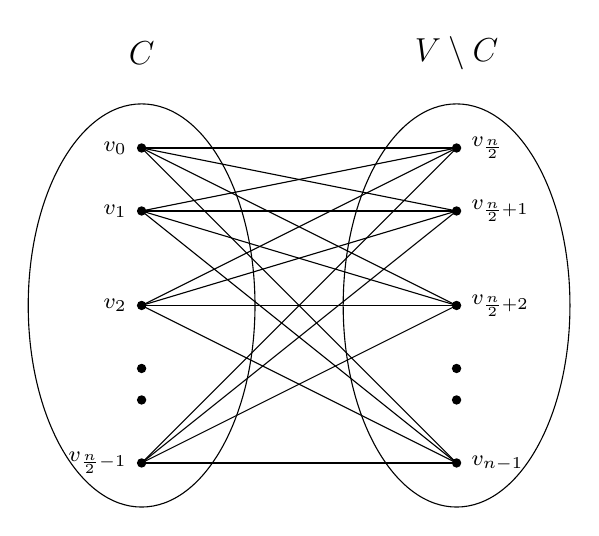
\begin{tikzpicture}[scale=0.8,
		every node/.style={font=\footnotesize},  %
		dot/.style={circle,fill,inner sep=1.2pt}
		]
		
		\draw (-6,5) ellipse (1.8 and 3.2);
		\draw (-11,5) ellipse (1.8 and 3.2);
		
		\node[dot,label=left:$v_0$] at (-11,7.5) {};
		\node[dot,label=left:$v_1$] at (-11,6.5) {};
		\node[dot,label=left:$v_2$] at (-11,5) {};
	
		\node[dot] at (-11,4) {};
		\node[dot] at (-11,3.5) {};
		\node[dot,label=left:$v_{\frac{n}{2}-1}$] at (-11,2.5) {};
		
	
		\node[dot,label=right:$v_{\frac{n}{2}}$] at (-6,7.5) {};
		\node[dot,label=right:$v_{\frac{n}{2}+1}$] at (-6,6.5) {};
		\node[dot,label=right:$v_{\frac{n}{2}+2}$] at (-6,5) {};
	\node[dot] at (-6,4) {};
		\node[dot] at (-6,3.5) {};
		\node[dot,label=right:$v_{n-1}$] at (-6,2.5) {};
		\draw (-11,7.5)--(-6,6.5);
		\draw (-11,7.5)--(-6,5);
		\draw (-11,6.5)--(-6,6.5);
		\draw (-11,6.5)--(-6,5);
		\draw (-11,5)--(-6,5);
		\draw (-11,5)--(-6,2.5);
		\draw (-11,2.5)--(-6,2.5);
		\draw (-11,2.5)--(-6,6.5);
		
	
		\draw (-6,7.5)--(-11,7.5);
		\draw (-6,7.5)--(-11,6.5);
		\draw (-6,7.5)--(-11,5);
		\draw (-6,7.5)--(-11,2.5);
		
	
		\draw (-11,7.5)--(-6,2.5);
		\draw (-11,6.5)--(-6,2.5);
		\draw (-11,5)--(-6,6.5);
		\draw (-11,2.5)--(-6,5);
	
		\node[font=\large] at (-11,9) {$C$};
		\node[font=\large] at (-6,9) {$V\setminus C$};
		
	\end{tikzpicture}
\caption{\footnotesize The bipartite graph obtained from a $(0,|S|)$-regular set.}	
\end{figure}
The resulting graph $\Gamma$ is bipartite. However, according to  Lemma~\ref{nonbipartite}, the graph $\Gamma$ is non-bipartite. Therefore, graph $\Gamma$  contains no $(0,|S|)$-regular set.This completes the proof. \hfill\bull
\end{proof}	
Now, we study the graph $\mathrm{Cay}(\mathbb{Z}_n, S)$, when  $|S|$ is odd and $|S|\geq3 $.
\begin{lem}\label{nonbipartite-odd}
	Let $\Gamma = \mathrm{Cay}(\mathbb{Z}_n, S)$ be a connected $|S|$-regular graph, where $|S|$ is odd, $|S|\geq3$ and $n$ is even. Suppose that there exist elements $x^t, x^r \in S$ such that $t$ is odd and $r$ is even. Then $\Gamma$ is not bipartite.	
\end{lem}
\begin{proof}
Assume, to the contrary, that $\Gamma$ is bipartite graph. By using Remark~\ref{rem:irr-rep} and Proposition~\ref{prop:eigenvalues-abelian}, the eigenvalues of $\Gamma = \mathrm{Cay}(\mathbb{Z}_n, S)$, with  $S = \{x^{k_1}, x^{-k_1}, \dots, x^{k_{\frac{|S|-1}{2}}}, x^{-k_{\frac{|S|-1}{2}}},x^{\frac{n}{2}}\}$ are computed as follows:

	\[
	\begin{aligned}
		\lambda_j &=
		e^{\frac{2 \pi \mathbf{i} j (k_1)}{n}}
		+ e^{\frac{2 \pi \mathbf{i} j (-k_1)}{n}}
		+ \cdots
		+ e^{\frac{2 \pi \mathbf{i} j (k_{\frac{|S|-1}{2}})}{n}}
		+ e^{\frac{2 \pi \mathbf{i} j (-k_{\frac{|S|-1}{2}})}{n}}
		+ e^{\frac{2 \pi \mathbf{i} j (\frac{n}{2})}{n}} \\
		&=
		\cos\left(\frac{2 \pi j k_1}{n}\right)
		+ \mathbf{i}\,\sin\left(\frac{2 \pi j k_1}{n}\right)
		+ \cos\left(\frac{2 \pi j k_1}{n}\right)
		- \mathbf{i}\,\sin\left(\frac{2 \pi j k_1}{n}\right)
		+ \cdots \\
		&\quad + \cos\left(\frac{2 \pi j k_{\frac{|S|-1}{2}}}{n}\right)
		+ \mathbf{i}\,\sin\left(\frac{2 \pi j k_{\frac{|S|-1}{2}}}{n}\right)
		+ \cos\left(\frac{2 \pi j k_{\frac{|S|-1}{2}}}{n}\right)
		- \mathbf{i}\,\sin\left(\frac{2 \pi j k_{\frac{|S|-1}{2}}}{n}\right) \\
	    &\quad 	+ (-1)^ j
    	\end{aligned}
          \]
Similar to Lemma~\ref{nonbipartite}, we have:

	\[
	\lambda_j
	= 2\left(
	\cos\!\left(\frac{2\pi j k_1}{n}\right)
	+ \cdots
	+ \cos\!\left(\frac{2\pi j k_{\frac{|S|-1}{2}}}{n}\right)
	\right) + (-1)^j
	= -|S| \;
	\]
Therefore
\begin{equation}\label{cos-sum-1}
	\lambda_j
	= \sum_{m=1}^{\frac{|S|-1}{2}}
	\cos\!\left(\frac{2\pi j k_m}{n}\right)
	= \frac{-|S|-(-1)^j}{2},
	\qquad 0 < j \le n-1
\end{equation}	
Since $ -1 \le \cos(\theta) \le 1$, it follows that relation \eqref{cos-sum-1} lies between the following two values:
    \[
     \frac{-|S|+1}{2} \le \frac{-|S|-(-1)^j}{2} \le \frac{|S|-1}{2}
    \]
We now consider two cases:\\
Case 1: If $j$ is even, we have:
    \begin{equation}\label{$|S|$}
     \frac{-|S|+1}{2} \le \frac{-|S|-1}{2} \le \frac{|S|-1}{2}	
   \end{equation}
   Ineqeality relation \eqref{$|S|$} does not hold.\\
   Case 2: If $j$ is odd, we have:
   	 \begin{equation}\label{$|S|$-odd}
   		\frac{-|S|+1}{2} \le \frac{-|S|+1}{2} \le \frac{|S|-1}{2}	
   	\end{equation}
relation \eqref{$|S|$-odd} holds for $|S|\geq3 $, and may have a solution only when, $
\cos\left(\frac{2\pi j k_1}{n}\right)
= \cdots
= \cos\left(\frac{2\pi j k_{\frac{|S|-1}{2}}}{n}\right)
= -1$. Analogous to Lemma~\ref{nonbipartite}, we obtain, $k_t \left( 2 d_r + 1 \right) = k_r \left( 2 d_t + 1 \right)$. Since, $k_t$ is odd and $k_r$ is even, we have $k_t (2 d_r + 1) \neq k_r (2 d_t + 1)$, leading to a contradiction. Therefore, the graph $\Gamma$ is not bipartite. This completes the proof. \hfill\bull
	\end{proof}
\begin{thm}\label{no-regular-set-odd}
Let $\Gamma = \mathrm{Cay}(\mathbb{Z}_n, S)$ be a connected $|S|$-regular graph, where $|S|$ is odd, $|S|\geq3 $ and $n$ is even. Suppose that  there exist elements $x^t, x^r \in S$ such that $t$ is odd and $r$ is even. Then $\Gamma$ contains no $(0,|S|)$-regular set.		
\end{thm}
\begin{proof}	
This result is proved using Lemma~\ref{nonbipartite-odd} and by an argument analogous to that of theorem~\ref{no-regular-set}.\hfill\bull   	
\end{proof}
Now, we give the main result in this section, which gives a necessary and sufficient condition for $\mathrm{Cay}(\mathbb{Z}_n, S)$ to admit a $(0,|S|)$-regular sets.

\begin{thm}\label{admit-$(0,|S|)$}
Let $\Gamma = \mathrm{Cay}(\mathbb{Z}_n, S)$ be a connected $|S|$-regular graph, such that all elements of $S$	are odd. Then $\Gamma$ contains a $(0,|S|)$-regular set if and only if $n$ is even.
\end{thm}
\begin{proof}
	We first show the necessity. Suppose that the graph $\Gamma$ contains a $(0,|S|)$-regular set $C$. We prove that $n$ is divisible by 2. By applying the trivial character to relation \eqref{C-S}, we obtain,  $2 |C| = n$. Therefore, $n$ is a multiple of 2. Now, we prove the sufficiency. Suppose that $n$ and $|S|$ the numbers are even. We define:
	\[
	\Gamma_1 = \mathrm{Cay}(\mathbb{Z}_n, \{x^{k_1}, x^{-k_1}, \dots, x^{k_{\frac{|S|}{2}}}, x^{-k_{\frac{|S|}{2}}}\})
	\]
	We prove that the graph $\Gamma_1$ contains a $(0,|S|)$-regular set. Since all elements of the set $S$ are odd, we have:
	 \[
\overline{S} = x^{2p_1+1}+x^{-2p_1-1}+ \dots+ x^{2p_\frac{|S|}{2} + 1}+x^{-2p_\frac{|S|}{2} - 1}
	 \]
We show that $C=\langle x^2 \rangle$ is a $(0,|S|)$-regular set for the graph  $\Gamma_1$. Therefore, the set $C$ must satisfy relation \eqref{C-S}. We have:
\[
(x^{2p_1+1}+x^{-2p_1-1}+ \dots+ x^{2p_\frac{|S|}{2} + 1}+x^{-2p_\frac{|S|}{2} - 1}) (\overline{\langle x^2 \rangle})\, +  |S|(\overline{\langle x^2 \rangle}) = |S|(x\, \overline{\langle x^2 \rangle}\,+ \overline{\langle x^2 \rangle})
\]
Since $n$ is even, it follows that, $\overline{\mathbb{Z}_n} \ = \overline{\langle x^2 \rangle} + x\,\overline{\langle x^2 \rangle}$. Therefore, $C$ is a $(0,|S|)$-regular set for the $\Gamma_1$. Now, suppose that $|S|$ is odd and let
	\[
\Gamma_2 = \mathrm{Cay}(\mathbb{Z}_n, \{x^{k_1}, x^{-k_1}, \dots, x^{k_{\frac{|S|-1}{2}}}, x^{-k_{\frac{|S|-1}{2}}}, x^{\frac{n}{2}}\})
\]
We have, $\overline{S} = x^{2p_1+1}+x^{-2p_1-1}+ \dots+ x^{2p_\frac{|S|-1}{2} + 1}+x^{-2p_\frac{|S|-1}{2}-1} + x^{2 z + 1}$. Similarly, $|S|$ even, provide $C=\langle x^2 \rangle$ is a $(0,|S|)$-regular set for the graph  $\Gamma_2$. This completes the proof.\hfill\bull 	
\end{proof}

Combining Corollary~\ref{nonbipartite-4}, Theorem~\ref{no-regular-set} and Theorem~\ref{admit-$(0,|S|)$}, we obtain the following result for $\Gamma = \mathrm{Cay}(\mathbb{Z}_n, \{x^k, x^{-k}, x^\ell, x^{-\ell}\})$.
\begin{cor}\label{$(0,4)$-regular set}
	Let $n, k, \ell$ be positive integers, and  $\Gamma = \mathrm{Cay}(\mathbb{Z}_n, \{x^k, x^{-k}, x^\ell, x^{-\ell}\})$ be a connected circulant quartic graph. Then the following statements hold:
	\begin{enumerate}
		\item[(i)] If $k \equiv 1 \pmod{2}$ and $\ell \equiv 0 \pmod{2}$, then the graph $\Gamma$ contains no $(0,4)$-regular set.
		\item[(ii)] If $k \equiv 1 \pmod{2}$ and $\ell \equiv 1 \pmod{2}$, then the graph $\Gamma$ contains a $(0,4)$-regular set if and only if $n$ is a multiple of $2$.
	\end{enumerate}	
	\end{cor}
\begin{example}\label{Cay-$(0,|S|)$}
Cayley graphs
\[
\begin{aligned}
   &\Gamma_1 = \mathrm{Cay}(\mathbb{Z}_6, \{x^1, x^5, x^3\}), \Gamma_2 = \mathrm{Cay}(\mathbb{Z}_8, \{x^1, x^7, x^5,  x^3\})\\
     &\Gamma_3 = \mathrm{Cay}(\mathbb{Z}_{10}, \{x^3, x^7, x^5, x^9,x^1\}), \Gamma_4 = \mathrm{Cay}(\mathbb{Z}_{12}, \{x^1, x^{11}, x^3, x^9, x^5, x^7\})
\end{aligned}
\]
 with set $C=\langle x^2 \rangle$, have $(0,|S|)$-regular set. Graph $\Gamma_1$ has a $(0,3)$-regular set, graph  $\Gamma_2$ has a $(0,4)$-regular set, graph  $\Gamma_3$ has a $(0,5)$-regular set, graph  $\Gamma_4$ has a $(0,6)$-regular set.
\end{example}

\section{\bf $(1,|S|)$ and $(|S|,0)$-regular sets}
\quad In this section, we will examine $(1,|S|)$-regular set and $(|S|,0)$-regular set. First, we examine $(1,|S|)$-regular set and show that in $\Gamma = \mathrm{Cay}(G, S)$, under the conditions imposed on the set $S$ in the following theorem, there is no $(1,|S|)$-regular set. Moreover, by Lemma~\ref{primes} the complement of a $(1,|S|)$-regular set namely $(0,|S|-1)$-regular set not exist either. As a result we show that graph $\Gamma = \mathrm{Cay}(\mathbb{Z}_n, \{x^k, x^{-k}, x^\ell, x^{-\ell}\})$ does not contain any $(1,4)$-regular set.
\begin{thm}\label{$(1,|S|)$}
	Let $G$ be a group, $S$ an inverse-closed subset of $G \setminus \lbrace e \rbrace$, and $\Gamma = \mathrm{Cay}(G, S)$ be a connected $|S|$-regular graph, where  $|S|\geq3$ and $S$ is closed under conjugation. Then $\Gamma$ contains no $(1,|S|)$-regular set.
\end{thm}
\begin{proof}
	By way of contradiction, assume that $C$ is a $(1,|S|)$-regular set of $\Gamma$. According to the definition of a $(1,|S|)$-regular set, we have:
	\[
	|N(v)\cap C| = 1 \qquad \forall\, v \in C
	\]
	\[
	|N(v)\cap C| = |S| \qquad \forall\, v \notin C
	\]
	without loss of generality, assume that $p$ and $q$ are two adjacent vertices in $C$, with $p\neq q$. Then we have:
	\begin{align*}
	 N(p)=\lbrace ps |s \in S\rbrace = pS\\
	 N(q)=\lbrace qs |s \in S\rbrace = qS
	 \end{align*}
	Suppose $k = p^{-1} q$, where $k\in S$. Since $S$ is an inverse-closed subset of $G \setminus \lbrace e \rbrace$, it follows that $k^{-1} \in S$ and $k \neq k^{-1}$.  Suppose that there exists $\ell \in S$ such that $\ell \neq k, k^{-1}$. Then the two vertices $p\ell$ and $q\ell$, with $p\ell \neq ql$, are adjacent to each other, because $(p\ell)^{-1} (q\ell) = \ell ^ {-1} p^{-1} q\ell = \ell ^{-1} k \ell$. By assumption, the subset $S$ of the group $G$ is closed under conjugation. Hence, $\ell ^{-1} k \ell \in S$. We now show that $p\ell \neq q$ and $q\ell \neq p$ and $p\ell, q\ell \notin C$. First, we show that $p\ell \neq q$ and $q\ell \neq p$. Suppose that $p\ell = q$, then we have, $p\ell = q \Rightarrow \ell = p^{-1} q \Rightarrow \ell = k $, which is a contradiction, because $\ell \neq k $. Suppose that $q\ell =p$. Then we have, $q\ell = p \Rightarrow \ell = q^{-1} p$. On the other hand, we have $k = p^{-1} q$ and computing $k^{-1}$, gives $k^{-1}=(p^{-1} q) ^{-1} = q^{-1} p$. Thus $\ell = k^{-1}$, which is a contradiction, because $\ell \neq k ^{-1}$. We now show that $p\ell, q\ell \notin C $. Suppose that $p\ell \in C$. On the other hand $p\ell \in pS$, since $pS = \lbrace ps |s \in S\rbrace$ and $\ell \in S$ hence, $p\ell \in pS$ and is adjacent to $p$. By assumption, the vertex $p\in C$ is adjacent to $q$. If $p\ell$ were also in $C$, then $p$ would be adjacent to both $q$ and $p\ell$, which contradictions the condition that $ |N(v)\cap C| = 1 $ for every $v \in C$, therefore $p\ell \notin C$. We now prove that $q\ell \notin C$. Suppose that $q\ell \in C$. In this case, $q\ell \in qS$ and is a neighbor of $q$ in $C$. Then the vertex $q$ would be adjacent to both $p$ and $q\ell$ in $C$, which contradict the condition $ |N(v)\cap C| = 1 $ for every $v \in C$. Therefore, both $p\ell$ and $q\ell$ are adjacent vertices in $V \setminus C$. Since the graph $\Gamma$ is $|S|$-regular, the vertex $p \ell$ can be adjacent to at most $|S|-1$ other vertices, on the other hand $ |N(v)\cap C| = |S| $ for every $v \in V \setminus C $. However, the vertex $p\ell$ can be adjacent to at most $|S|-1$ vertices in $C$, which is a contradiction. Hence no $(1,|S|)$-regular set exists. This completes the proof.\hfill\bull
	\end{proof}
The following corollary follows from Theorem~\ref{$(1,|S|)$}.

\begin{cor}\label{$(1,4)$-regular set}
	Let $n, k, \ell$ be positive integers, and  $\Gamma = \mathrm{Cay}(\mathbb{Z}_n, \{x^k, x^{-k}, x^\ell, x^{-\ell}\})$ be a connected circulant quartic graph. Then the graph $\Gamma$ contains no $(1,4)$-regular set.
	\end{cor}
	Now, we study the $(|S|,0)$-regular set in $\mathrm{Cay}(\mathbb{Z}_n, S)$ in two cases: when $|S|$ is even and when $|S|$ is odd. First, we show that $\mathrm{Cay}(\mathbb{Z}_n, S)$ for even $|S|$ does not contain any $(|S|,0)$-regular set. We state the following lemma, which will be used in the proof of the theorem.
	\begin{lem}\label{X=Y}
		Let $G$ be a finite abelian group, $X$ and $Y$ be two nonempty subsets of $G$ of equal size. Then for each irreducible character $\chi$ of $G$ we have $\sum\limits_{x \in X} x ^ \chi = \sum\limits_{y \in Y} y ^ \chi$ if and only if $X=Y$.
		\end{lem}
\begin{thm}\label{$(|S|,0)$}
Let  $\Gamma = \mathrm{Cay}(\mathbb{Z}_n, S)$ be a connected $|S|$-regular graph, where $|S|$ is even. Then $\Gamma$ contains no $(|S|,0)$-regular set.	
\end{thm}	
	\begin{proof}
		For a proof by contradiction, suppose that the graph $\Gamma$ contains a $(|S|,0)$-regular set $C$. Assume that $S = \{x^{k_1}, x^{-k_1}, \dots, x^{k_{\frac{|S|}{2}}}, x^{-k_{\frac{|S|}{2}}}\}$. By applying the nontrivial irreducible characters of the group $\mathbb{Z}_n$ on the equation Lemma~\ref{Z}~(iv), we obtain, $\overline{C}^{\chi_m} (\overline{S}^{\chi_m}+(b-a))= b\;\overline{\mathbb{Z}_n}^{\chi_m}$ for each  $1 \le m \le n-1$. Since $\mathbb{Z}_n = \langle x \rangle $ is an abelian group, we have $\overline{\mathbb{Z}_n}^{\chi_m} = 0$ for every  $1 \le m \le n-1$. Therefore in the $(|S|,0)$-regular case we obtain:
		\begin{equation}\label{S-|S|}
		\overline{C}^{\chi_m} (\overline{S}^{\chi_m}-|S|)= 0, \qquad 1 \le m \le n-1
		\end{equation}
	we have:
	\[
	\begin{aligned}
		\overline{S}^{\chi_m} &=
		e^{\frac{2 \pi \mathbf{i} m (k_1)}{n}}
		+ e^{\frac{2 \pi \mathbf{i} m (-k_1)}{n}}
		+ \cdots
		+ e^{\frac{2 \pi \mathbf{i} m (k_{\frac{|S|}{2}})}{n}}
		+ e^{\frac{2 \pi \mathbf{i} m (-k_{\frac{|S|}{2}})}{n}} \\
		&=
		\cos\left(\frac{2 \pi m k_1}{n}\right)
		+ \mathbf{i}\,\sin\left(\frac{2 \pi m k_1}{n}\right)
		+ \cos\left(\frac{2 \pi m k_1}{n}\right)
		- \mathbf{i}\,\sin\left(\frac{2 \pi m k_1}{n}\right)
		+ \cdots \\
		&\quad + \cos\left(\frac{2 \pi m k_{\frac{|S|}{2}}}{n}\right)
		+ \mathbf{i}\,\sin\left(\frac{2 \pi m k_{\frac{|S|}{2}}}{n}\right)
		+ \cos\left(\frac{2 \pi m k_{\frac{|S|}{2}}}{n}\right)
		- \mathbf{i}\,\sin\left(\frac{2 \pi m k_{\frac{|S|}{2}}}{n}\right)
	\end{aligned}
	\]	
	Therefore
	\[
	\overline{S}^{\chi_m} = 2	\sum_{j=1}^{\frac{|S|}{2}}
	\cos\!\left(\frac{2\pi m k_j}{n}\right),
	\qquad 1 \le m \le n-1
	\]	
	From relation\eqref{S-|S|} we have $\overline{C}^{\chi_m} = 0$ or  $(\overline{S}^{\chi_m}-|S|) = 0$. Suppose that   $(\overline{S}^{\chi_m}-|S|) = 0$, for each $1 \le m \le n-1$. Therefore, $\sum_{j=1}^{\frac{|S|}{2}}
	\cos\!\left(\frac{2\pi j k_j}{n}\right)
	= \frac{|S|}{2}$ and it follows that $\cos\left(\frac{2\pi m k_1}{n}\right)
	= \cdots
	= \cos\left(\frac{2\pi m k_{\frac{|S|}{2}}}{n}\right)
	= 1$ for each $1 \le m \le n-1$, then
	\[
	\forall\, j \in \left\{1, \ldots, \frac{|S|}{2}\right\},
	\ \exists\, d_j \in \mathbb{Z} :
	\frac{2\pi m k_j}{n} = 2 d_j \pi
	\;\Longrightarrow\;
	\frac{m k_j}{n} = d_j\;\Longrightarrow\
	\]
	\begin{equation}\label{n mid m}
	 n \mid m\;k_1, \ldots, m\;k_{\frac{|S|}{2}} \Longrightarrow\; n \mid m  \gcd(k_1,\dots, k_{\frac{|S|}{2}})
	\end{equation}
	Since the graph $\Gamma$ is $|S|$-regular and connected from Lemma~\ref{CayC} we proved that $\gcd(k_1,\ldots,k_{\frac{|S|}{2}})=1$. By relation\eqref{n mid m}, we have $n \mid m$. On the other hand, $1 \le m \le n-1$ and $n \nmid m$. Hence $(\overline{S}^{\chi_m}-|S|) \neq 0$ and $\overline{C}^{\chi_m}$ must be equal to zero. That is $\overline{C}^{\chi_m} = \sum\limits_{c \in C} c =0 $ for each $1 \le m \le n-1$. It is clear that for every $x^i \in \mathbb{Z}_n$, where $ 0 \le i \le n-1$ we have $\overline{x^i C}^{\chi_m} = 0$ for $1 \le m \le n-1 $. By applying the trivial character to $\overline{ C}$ and $\overline{x^i C}$ for $0 \le i \le n-1 $, we have $\overline{C}^{\chi_0} = \overline{x^i C}^{\chi_0} = |C|$. Clearly $|x^i C| = |C|$ and by Lemma~\ref{X=Y} for each $i \in \{0,1,\ldots,n-1\}$ we have $x^i C = C$. Since $1 \in C$ it follows that $C = \mathbb{Z}_n $, this is a contradiction, because a regular set must be non-empty and the graph $\Gamma$ contains no $(|S|,0)$-regular set. This completes the proof.\hfill\bull
		\end{proof}
		The following corollary follows from Theorem~\ref{$(|S|,0)$}.
	\begin{cor}\label{$(4,0)$-regular set}
		Let $n, k, \ell$ be positive integers, and  $\Gamma = \mathrm{Cay}(\mathbb{Z}_n, \{x^k, x^{-k}, x^\ell, x^{-\ell}\})$ be a connected circulant quartic graph. Then the graph $\Gamma$ contains no $(4,0)$-regular set. 		
	\end{cor}
	Now we consider the case of $\mathrm{Cay}(\mathbb{Z}_n, S)$ where $|S|$ is odd and $|S|\geq3$.
	\begin{thm}\label{$(|S|,0)Sodd$}
	Let $\Gamma = \mathrm{Cay}(\mathbb{Z}_n, S)$ be a connected $|S|$-regular graph, where $|S|$ is odd, $|S|\geq3 $ and $n$ is even. Then $\Gamma$ contains no $(|S|, 0)$-regular set.
      \end{thm}	
    \begin{proof}
    By contradiction, let us assume that the graph $\Gamma$ contains a $(|S|,0)$-regular set $C$. Let  $S = \{x^{k_1}, x^{-k_1}, \dots, x^{k_{\frac{|S|-1}{2}}}, x^{-k_{\frac{|S|-1}{2}}},x^{\frac{n}{2}}\}$. Similarly, and using the argument applied in Theorem~\ref{$(|S|,0)$}, we have:	
    \begin{equation}\label{S-|S|-S}
    	\overline{C}^{\chi_m} (\overline{S}^{\chi_m}-|S|)= 0, \qquad 1 \le m \le n-1
    \end{equation}
    By computing $\overline{S}^{\chi_m}$, we obtain that:
    \[
    \overline{S}^{\chi_m} = 2	\sum_{j=1}^{\frac{|S|-1}{2}}
    \cos\!\left(\frac{2\pi m k_j}{n}\right) + (-1)^m,
    \qquad 1 \le m \le n-1
    \]
    From relation\eqref{S-|S|-S} we have $\overline{C}^{\chi_m} = 0$ or  $(\overline{S}^{\chi_m}-|S|) = 0$. Suppose that   $(\overline{S}^{\chi_m}-|S|) = 0$ for each  $1 \le m \le n-1$. Therefore
    \begin{equation}\label{cos-sum-2}
     \sum_{j=1}^{\frac{|S|-1}{2}}
    	\cos\!\left(\frac{2\pi m k_j}{n}\right)
    	= \frac{|S|-(-1)^m}{2},
    	\qquad 1 \le m\le n-1
    \end{equation}	
    Since $ -1 \le \cos(\theta) \le 1$, it follows that relation \eqref{cos-sum-2} lies between the following two values:
    \[
    \frac{-|S|+1}{2} \le \frac{|S|-(-1)^m}{2} \le \frac{|S|-1}{2}
    \]
    We now consider two cases:\\
    Case 1: If $m$ is odd, we have:
    \begin{equation}\label{a1}
    	\frac{-|S|+1}{2} \le \frac{|S|+1}{2} \le \frac{|S|-1}{2}	
    \end{equation}
    Ineqeality relation\eqref{a1} does not hold.\\
    Case 2: If $m$ is even, we have:
    \begin{equation}\label{a2}
    	\frac{-|S|+1}{2} \le \frac{|S|-1}{2} \le \frac{|S|-1}{2}	
    \end{equation}
    relation\eqref{a2} holds for $|S|\geq3 $, and may have a solution only when
    \[
    \cos\left(\frac{2\pi m k_1}{n}\right) = \dots = \cos\left(\frac{2\pi m  k_{\frac{|S|-1}{2}}}{n}\right) = 1
    \]
    Similar to  Theorem~\ref{$(|S|,0)$} we obtain that
     $ n \mid m  \gcd(k_1,\dots, k_{\frac{|S|-1}{2}})$ and we may write $m \gcd(k_1,\dots, k_{\frac{|S|-1}{2}}) = nt$, for some integer $t$ and consequently $\frac{nt}{m}$ is a positive integer. Since $m$ is an even integer and $1 \le m \le n-1$, we have:
     \begin{equation}\label{eq:gcd}
     	\begin{aligned}
     	\gcd\!\left(k_1,\ldots,k_{\frac{|S|-1}{2}},\frac{n}{2}\right)
     	&=\gcd\!\left(\gcd\!\left(k_1,\ldots,k_{\frac{|S|-1}{2}}\right),\frac{n}{2}\right)
     	\\
     	&=\gcd\!\left(\frac{nt}{m},\frac{n}{2}\right)
     	\\
     	&=\frac{n}{m}\gcd\!\left(t,\frac{m}{2}\right)
    	\end{aligned}
    \end{equation}
    On the other hand the graph $\Gamma$ is $|S|$-regular and connected and according to Lemma~\ref{CayC} we obtained that $\gcd(k_1,\dots, k_{\frac{|S|-1}{2}}, \frac{n}{2}) = 1$. Therefore by relation\eqref{eq:gcd} we have $n \gcd(t,\frac{m}{2}) = m$ which implies that $n|m$ for $1 \le m \le n-1$ leading to a contradiction. Hence $(\overline{S}^{\chi_m}-|S|) \neq 0$ and similarly to Theorem~\ref{$(|S|,0)$} it is proved that $\overline{C}^{\chi_m} \neq 0$ for $0 \le m \le n-1$. Therefore the graph $\Gamma$ contains no $(|S|,0)$-regular set. This completes the proof.\hfill\bull  	
    	\end{proof}
   \section{The remaining cases of $(a,b)$-regular sets in circulant quartic graphs}

  \quad This section is devoted to the study of the remaining cases of $(a,b)$-regular sets in circulant quartic graphs. It consists of three subsections, each of which is devoted to one of the remaining cases. In each subsection, the technique of applying group homomorphisms is used to prove the nonexistence of the specified $(a,b)$-regular sets. Finally, by exploiting properties of primitive roots of unity, we examine the invertibility of the resulting circulant matrices. We also provide necessary and sufficient conditions for the existence of the specified $(a,b)$-regular sets in each subsection. We first present the necessary lemmas and theorems for the subsequent subsections.

  \begin{lem}\label{samecoset}
  	Let $\mathbb{Z}_n=\langle x\rangle$ be a cyclic group of order $n$, and let $p$ be a prime number and $\alpha$ be a positive integer such that $p^{\alpha}\mid n$. Suppose that $H=\langle x^{p^{\alpha}}\rangle$ is a subgroup of $\mathbb{Z}_n$. Then for every positive integer $\ell$, the two elements $x^{\ell}$ and $x^{-\ell}$ belong to the same coset of $H$ if and only if $p^{\alpha}\mid2\ell$.
  \end{lem}

  \begin{proof}
  	Assume that the two elements $x^{\ell}$ and $x^{-\ell}$ belong to the same coset of $H$. It suffices to show that $p^{\alpha}\mid2\ell$. We have
  	\begin{equation}\label{samecoset1}
  		x^{\ell}H=x^{-\ell}H\rightarrow x^{-2\ell}\in H\rightarrow x^{-2\ell}=\left(x^{p^{\alpha}}\right)^{t_1}
  	\end{equation}
  	
    \noindent Since $x$ is a generator of the cyclic group $\mathbb{Z}_n$, we have $\operatorname{ord}(x)=n$, and since $p^{\alpha}\mid n$, we have $n=p^{\alpha}t_2$ for some integer $t_2$. By relation~\eqref{samecoset1}, we have
  	
  	\[
  	-2\ell\stackrel{p^{\alpha}t_2}{\equiv}p^{\alpha}t_1
  	\rightarrow
  	p^{\alpha}t_2\mid(-2\ell-p^{\alpha}t_1)
  	\rightarrow
  	p^{\alpha}\mid2\ell
  	\]
  	
  	\noindent Conversely, assume that $p^{\alpha}\mid2\ell$. We show that the two elements $x^{\ell}$ and $x^{-\ell}$ belong to the same coset of the subgroup $H$. It suffices to show that $x^{2\ell}\in H$. We have
  	
  	\[
  	p^{\alpha}\mid2\ell
  	\rightarrow
  	\exists\,t_3\in\mathbb{Z}:2\ell=p^{\alpha}t_3
  	\rightarrow
  	x^{2\ell}=x^{p^{\alpha}t_3}
  	\]
  	
  	\noindent Hence, $x^{2\ell}\in H$. This completes the proof.
  	\hfill$\blacksquare$
  \end{proof}
  The following corollaries are immediate consequences of Lemma~\ref{samecoset}.

  \begin{cor}\label{oddprime}
  	Under the assumptions of Lemma~\ref{samecoset}, if $p$ is an odd prime, then the two elements $x^\ell$ and $x^{-\ell}$ belong to the same coset of $H$ if and only if $p^\alpha\mid\ell$.
  \end{cor}

  \begin{cor}\label{power2}
  	Under the assumptions of Lemma~\ref{samecoset}, if $p=2$, then the two elements $x^\ell$ and $x^{-\ell}$ belong to the same coset of $H$ if and only if $2^{\alpha-1}\mid\ell$.
  \end{cor}
  \begin{lem}\label{samecoset2}
  	Let $\mathbb{Z}_n=\langle x\rangle$ be a cyclic group of order $n$, and let $p$ be a prime number, and $\alpha$ be a positive integer. Suppose that $H=\langle x^{p^\alpha}\rangle$ is a subgroup of $\mathbb{Z}_n$. Then the two elements $x^k$ and $x^\ell$ belong to the same coset of $H$ if and only if $x^{k-\ell}\in H$.
  \end{lem}

  \begin{proof}
  	Assume that the two elements $x^k$ and $x^\ell$ belong to the same coset of $H$. It suffices to show that $x^{k-\ell}\in H$. By assumption, there exist $h_1,h_2\in H$ and an integer $d$ such that $x^k=x^dh_1$ and $x^\ell=x^dh_2$. Hence,
  	
  	\[
  	x^k(x^\ell)^{-1}
  	=(x^dh_1)(h_2^{-1}x^{-d})
  	=x^d(h_1h_2^{-1})x^{-d}
  	=h_1h_2^{-1}\in H.
  	\]
  	
  	Therefore, $x^{k-\ell}\in H$.
  	
  	\noindent Conversely, assume that $x^{k-\ell}\in H$. We show that $x^k$ and $x^\ell$ belong to the same coset of $H$. Since $x^k=x^\ell x^{k-\ell}$ and $x^{k-\ell}\in H$, it follows that $x^k\in x^\ell H$. Hence, $x^kH=x^\ell H$. Therefore, the two elements $x^k$ and $x^\ell$ belong to the same coset of $H$. This completes the proof.
  	\hfill$\blacksquare$
  \end{proof}
  \begin{prop}\label{prop:coset}
  	Let $\mathbb{Z}_n=\langle x\rangle$ be a cyclic group of order $n$, and let $p$ is a prime number, and $\alpha$ be a positive integer such that $p^\alpha\mid n$. Suppose that $H=\langle x^{p^\alpha}\rangle$ is a subgroup of $\mathbb{Z}_n$. Then for every positive integer $\ell$, $x^\ell\in x^dH$ for $0\le d\le p^\alpha-1$ if and only if $\ell\equiv d\pmod{p^\alpha}$.
  \end{prop}

  \begin{proof}
  	Assume that $x^\ell\in x^dH$ for $0\le d\le p^\alpha-1$. We show that $\ell\stackrel{p^\alpha}{\equiv} d$. We have
  	\[
  	x^\ell\in x^dH
  	\Longrightarrow
  	x^\ell\in\{x^{d+p^\alpha m}\mid m\in\mathbb Z\}.
  	\]
  	
  \noindent	Suppose that
  	\[
  	\exists\,m_1\in\mathbb Z:\;
  	x^\ell=x^{d+p^\alpha m_1}
  	\Longrightarrow
  	\ell \overset{p^\alpha t}{\equiv} d+p^\alpha m_1
  	\Longrightarrow
  	p^\alpha t\mid\ell-d-p^\alpha m_1
  	\Longrightarrow
  	\ell\stackrel{p^\alpha}{\equiv} d
  	\]
  \noindent	Conversely, assume that
  $\ell\equiv d\pmod{p^\alpha}$. We show that $x^\ell\in x^dH$ for $0\le d\le p^\alpha-1$. We have
  	\[
  	\ell\stackrel{p^\alpha}{\equiv} d
  	\Longrightarrow
  	p^\alpha\mid(\ell-d)
  	\Longrightarrow
  	p^\alpha m_2=\ell-d
  	\Longrightarrow
  	p^\alpha m_2+d=\ell
  	\Longrightarrow
  	x^\ell=x^{p^\alpha m_2+d}
  	\]
  \noindent	and this means that $x^\ell\in x^dH$. This completes the proof.
  \hfill$\blacksquare$
  \end{proof}
   \begin{lem}\label{nomulp}
  Let $\mathbb{Z}_n=\langle x\rangle$ be a cyclic group of order $n$, let $p$ be a prime number, and let $\alpha$ and $\ell$ be positive integers such that $p^\alpha\mid n$. Let $H=\langle x^{p^\alpha}\rangle$ be a subgroup of $\mathbb{Z}_n$. If $\ell\equiv1\pmod p$ and $x^\ell\in x^{r_\ell}H$ and $x^{-\ell}\in x^{r_{-\ell}}H$, then $p\nmid r_\ell$ and $p\nmid r_{-\ell}$.	
  \end{lem}
  \begin{proof}
  	According to Proposition~\ref{prop:coset}, we have
  	\begin{equation}\label{eq:lem66a}
  		x^\ell\in x^{r_\ell}\langle x^{p^\alpha}\rangle
  		\Longrightarrow
  		\ell\stackrel{p^\alpha}{\equiv} r_\ell
  		\Longrightarrow
  		\ell=p^\alpha m_1+r_\ell
  	\end{equation}
  	where $m_1\in\mathbb{Z}$. Since $\ell=pm_2+1$ for some $m_2\in\mathbb{Z}$, substituting $\ell$ into \eqref{eq:lem66a} yields
  	\[
  	pm_2+1=p^\alpha m_1+r_\ell
  	\Longrightarrow
  	p(m_2-p^{\alpha-1}m_1)=r_\ell-1
  	\Longrightarrow
  	r_\ell\stackrel{p}{\equiv} 1
  	\]
  	Hence, $p\nmid r_\ell$.
  	Now, for $-\ell$ we have
  	\begin{equation}\label{eq:lem66b}
  		x^{-\ell}\in x^{r_{-\ell}}H
  		\Longrightarrow
  		-\ell\stackrel{p^\alpha}{\equiv} r_{-\ell}	
  		\Longrightarrow
  		\ell=-p^\alpha m_3-r_{-\ell}
  	\end{equation}
  	where $m_3\in\mathbb{Z}$. Since $-\ell\equiv-1\pmod p$, we have $\ell=-pm_4-(p-1)$
  	for some $m_4\in\mathbb{Z}$. Substituting $\ell$ into \eqref{eq:lem66b} gives
  	\[
  	-pm_4-(p-1)=-p^\alpha m_3-r_{-\ell}
  	\Longrightarrow
  	p(-m_4+p^{\alpha-1}m_3)=p-1-r_{-\ell}
  	\Longrightarrow
  	p-1\stackrel{p}{\equiv} r_{-\ell}
  	\]
  	Hence, $p\nmid r_{-\ell}$.
   This completes the proof.\hfill$\blacksquare$
  \end{proof}
  \begin{prop}\label{prop:inverse_coset}
  	Let $\mathbb{Z}_n=\langle x\rangle$ be a cyclic group of order $n$, let $p$ be a prime number, and let $\alpha$ be a positive integer such that $p^\alpha\mid n$. Let $H=\langle x^{p^\alpha}\rangle$ be a subgroup of $\mathbb{Z}_n$. If $x^k\in x^dH$ for some integer $k$ and $0\le d\le p^\alpha-1$, then $x^{-k}\in x^{p^\alpha-d}H$.
  \end{prop}

  \begin{proof}
  	Assume that $x^k\in x^dH$. By the definition of a coset, there exists $h\in H$ such that $x^k=x^dh$. Since $H=\langle x^{p^\alpha}\rangle$, there exists an integer $t$ such that $h=x^{tp^\alpha}$. Hence, $x^k=x^{d+tp^\alpha}$, which implies that $k\equiv d\pmod{p^\alpha}$. Therefore, $-k\equiv-d\pmod{p^\alpha}$,  that is $-k=-d+sp^\alpha$ for some integer $s$. Thus, $x^{-k}=x^{-d}x^{sp^\alpha}$. Since $x^{sp^\alpha}\in H$, this implies that $x^{-k}\in x^{-d}H$. We have $x^{-d}H=x^{p^\alpha-d}H$, it follows that $x^{-k}\in x^{p^\alpha-d}H$. This completes the proof.\hfill$\blacksquare$
  \end{proof}

 \begin{cor}\label{cor:inverse_coset1}
 	Suppose that \(3\nmid k\) and \(x^k\in x^d\langle x^{3^\alpha}\rangle\), where \(1\leq d\leq3^\alpha-1\). Then \(x^{-k}\in x^{3^\alpha-d}\langle x^{3^\alpha}\rangle\). Moreover, if \(d\stackrel{3}{\equiv}1\), then \(3^\alpha-d\stackrel{3}{\equiv}-d\stackrel{3}{\equiv}-1\stackrel{3}{\equiv}2\). Similarly, if \(d\stackrel{3}{\equiv}2\), then \(3^\alpha-d\stackrel{3}{\equiv}1\).
 \end{cor}
  Using the argument in the proof of Theorem~\ref{khi3}, we obtain the following remark, which will be used throughout the subsequent subsections.
  \begin{rem}\label{rem:7}
  	Suppose that \(C\) is an \((a,b)\)-regular set for \(\Gamma=\operatorname{Cay}(\mathbb{Z}_n,S)\). Let \(p\) be a prime and let \(\alpha\) be a positive integer such that  \(p^{\alpha}\mid n\). Therefore, the homomorphism
  	\[
  	\begin{aligned}
  		\varphi:\; \mathbb{Z}_n &\longrightarrow \left\langle x^{\frac{n}{p^{\alpha}}}\right\rangle\\
  		z &\longmapsto z^{\frac{n}{p^{\alpha}}}
  	\end{aligned}
  	\]
    is well defined. Applying the homomorphism $\varphi$ to both sides of Equation~\eqref{eqq}, we obtain
  	\[
  	\left(\sum_{r=0}^{p^{\alpha}-1}s_rX^r\right)
  	\left(\sum_{h=0}^{p^{\alpha}-1}t_hX^h\right)
  	=
  	\frac{b\,n}{p^{\alpha}}
  	\left(\sum_{m=0}^{p^{\alpha}-1}X^m\right)
  	\]
  	where $	X:=x^{\frac{n}{p^{\alpha}}},\
  	(\bar{S}+(b-a))^{\varphi}
  	=
  	\sum_{r=0}^{p^{\alpha}-1}s_rX^r,\	(\bar{C})^{\varphi}
  	=
  	\sum_{h=0}^{p^{\alpha}-1}t_hX^h\ and\ s_r,t_h\in\mathbb{N}_0\, and\ s_0\in\mathbb{Z}.$ So we have:
  	\[
  	\begin{bmatrix}
  		s_0&s_1&\cdots&s_{p^{\alpha}-1}\\
  		s_1&s_2&\cdots&s_0\\
  		\vdots&\vdots&\ddots&\vdots\\
  		s_{p^{\alpha}-1}&s_0&\cdots&s_{p^{\alpha}-2}
  	\end{bmatrix}
  	\begin{bmatrix}
  		t_0\\
  		t_{p^{\alpha}-1}\\
  		\vdots\\
  		t_1
  	\end{bmatrix}
  	=
  	\frac{b\,n}{p^{\alpha}}
  	\begin{bmatrix}
  		1\\
  		1\\
  		\vdots\\
  		1
  	\end{bmatrix}
  	\]
  	where\ $ S_d := x^d \langle x^{p^{\alpha}} \rangle \cap S\ for\ 0 \le d \le p^{\alpha}-1, s_0:=\left|\left\langle x^{p^{\alpha}}\right\rangle\cap S\right|+(b-a),\ 	s_d:=\left|x^d\left\langle x^{p^{\alpha}}\right\rangle\cap S\right| for\ 1\le d\le p^{\alpha}-1\ and\ t_h:=\left|x^h\left\langle x^{p^{\alpha}}\right\rangle\cap C\right| for\ 0\le h\le p^{\alpha}-1.$
  \end{rem}
  In the following proposition, we shall use the notation $S_d$, $s_0$, and $s_d$ introduced in Remark~\ref{rem:7}.

  \begin{prop}\label{prop:podd}
  	Let $n$, $k$, $\ell$ be positive integers,
  	$
  	\Gamma=\operatorname{Cay}(\mathbb{Z}_n,\{x^k,x^{-k},x^\ell,x^{-\ell}\})
  	$
  	be a connected circulant quartic graph. Let $p$ is an odd prime, $\alpha$ be a positive integer such that $p^\alpha\mid n$, and
  	$
  	H=\langle x^{p^\alpha}\rangle.
  	$
  	Suppose that $C$ is an $(a,b)$-regular set in $\Gamma$ and
  	$
  	k\equiv1\pmod p,$ and
  $\ell\equiv1\pmod p.
  	$
  	Then the following statements hold:
 	\begin{enumerate}
  	\item[(i)] The two elements of each of the sets $\{x^k,x^{-k}\}$, $\{x^\ell,x^{-\ell}\}$, $\{x^k,x^{-\ell}\}$, and $\{x^{-k},x^\ell\}$ do not belong to the same coset of $H$.
  	\item[(ii)] If $p^\alpha \mid k-\ell$, then the two elements of each of the sets $\{x^k,x^\ell\}$ and $\{x^{-k},x^{-\ell}\}$ belong to the same coset of $H$.
 	\item[(iii)] If the two elements of each of the sets $\{x^k,x^\ell\}$ and $\{x^{-k},x^{-\ell}\}$ belong to the same coset of $H$, then
 	$
 	s_0=b-a,$ $s_{i_1}=s_{i_2}=2,
 	$
 	where $i_1$ and $i_2$ are distinct integers satisfying
 	$
 	1\le i_1,i_2\le p^\alpha-1.
 	$
  	\item[(iv)] If $\alpha\geq 2$, the two elements of each of the sets $\{x^k,x^\ell\}$ and $\{x^{-k},x^{-\ell}\}$ do not belong to the same coset of $H$, then
  	$
  	s_0=b-a,$ $ s_{i_1}=s_{i_2}=s_{i_3}=s_{i_4}=1,$
  	where $i_1$, $i_2$, $i_3$, and $i_4$ are pairwise distinct integers satisfying
  	$
  	1\le i_1,i_2,i_3,i_4\le p^\alpha-1.
  	$
  	\end{enumerate}
  \end{prop}
 \begin{proof}
\textbf{(i)} Since $k\stackrel{p}{\equiv}1$ and $\ell\stackrel{p}{\equiv}1$, we have $p^\alpha\nmid k$ and $p^\alpha\nmid \ell$. Therefore, by Corollary~\ref{oddprime}, the elements in each of the sets $\{x^k,x^{-k}\}$ and $\{x^\ell,x^{-\ell}\}$ do not belong to the same coset of $H$. Moreover, $k+\ell\stackrel{p}{\equiv}2$. Since $p$ is an odd prime, it follows that $p\nmid k+\ell$, and hence $p^\alpha\nmid k+\ell$. Therefore, $x^{k+\ell}\notin H$. By Lemma~\ref{samecoset2}, the elements $x^k$ and $x^{-\ell}$ do not belong to the same coset of $H$. Similarly, the elements $x^{-k}$ and $x^\ell$ do not belong to the same coset of $H$.

\textbf{(ii)} Assume that $p^\alpha\mid k-\ell$. Then $x^{k-\ell}\in H$. Hence, by Lemma~\ref{samecoset2}, the elements $x^k$ and $x^\ell$ belong to the same coset of $H$. Moreover, $p^\alpha\mid \ell-k $, and we have $x^{\ell-k}\in H$. Therefore, by Lemma~\ref{samecoset2}, the elements $x^{-k}$ and $x^{-\ell}$ also belong to the same coset of $H$.

\textbf{(iii)} Since $k\stackrel{p}{\equiv}1$ and $\ell\stackrel{p}{\equiv}1$, it follows that none of the elements $x^k$, $x^{-k}$, $x^\ell$, and $x^{-\ell}$ belongs to $H$. Therefore, $S\cap H=\varnothing$. By the definition of $s_0$ in Remark~\ref{rem:7} we have $s_0=|S\cap H|+b-a=b-a$. Moreover, by the assumption in part~(iiii), we have 	
\[
\exists\, d_1\in\{1,\ldots,p^{\alpha}-1\} :
\{x^{k},x^\ell\}\subseteq S_{d_1}
\]
\[
\exists\, d_2\in\{1,\ldots,p^{\alpha}-1\} :
\{x^{-k},x^{-\ell}\}\subseteq S_{d_2}
\]
These two cosets are distinct; otherwise, $x^k$ and $x^{-k}$ would belong to the same coset of $H$, contradicting part~(i). Therefore,
by the definition of $s_d$ in Remark~\ref{rem:7}, there exist distinct positive integers $i_1$ and $i_2$ in $\{1,\ldots,p^\alpha-1\}$ such that $s_{i_1}=s_{i_2}=2$.

\textbf{(iv)} Similar to part~(iii), we have $s_0=b-a$. Assume that $x^k\in S_{i_1}$, $x^{-k}\in S_{i_2}$, $x^\ell\in S_{i_3}$, and $x^{-\ell}\in S_{i_4}$ for some $i_1, i_2, i_3, i_4 \in \{1,\ldots,p^{\alpha}-1\}$. By part~(i), we have $i_1\neq i_2$, $i_3\neq i_4$, $i_1\neq i_4$, and $i_2\neq i_3$. Moreover, by the assumption of part~(iv), $i_1\neq i_3$ and $i_2\neq i_4$. Therefore, $i_1, i_2, i_3, i_4$ are pairwise distinct. By Remark~\ref{rem:7}, it follows that $s_{i_1}=s_{i_2}=s_{i_3}=s_{i_4}=1$. \hfill$\blacksquare$	
 	\end{proof}
 	
   \begin{prop}\label{prop:even2}
 	Let $n$, $k$, $\ell$ be positive integers,
 	$
 	\Gamma=\operatorname{Cay}(\mathbb{Z}_n,\{x^k,x^{-k},x^\ell,x^{-\ell}\})
 	$
 	be a connected circulant quartic graph. Let $\alpha\ge2$ be a positive integer such that $2^\alpha\mid n$, and
 	$H=\langle x^{2^\alpha}\rangle$.
 	Suppose that $C$ is an $(a,b)$-regular set in $\Gamma$ and
 	$
 	k\equiv1\pmod 2,$ and
 	$\ell\equiv1\pmod 2.
 	$
 	Then the following statements hold:
 	\begin{enumerate}
 		\item[(i)] The two elements of each of the sets $\{x^k,x^{-k}\}$, $\{x^\ell,x^{-\ell}\}$, do not belong to the same coset of $H$.
 		\item[(ii)] If $2^\alpha \mid k-\ell$, then the two elements of each of the sets $\{x^k,x^\ell\}$ and $\{x^{-k},x^{-\ell}\}$ belong to the same coset of $H$.
 		\item[(iii)] If $2^\alpha \mid k+\ell$, then the two elements of each of the sets $\{x^k,x^{-\ell}\}$ and $\{x^{-k},x^{\ell}\}$ belong to the same coset of $H$.
 		\item[(iv)] If the two elements of each of the sets $\{x^k,x^\ell\}$ and $\{x^{-k},x^{-\ell}\}$, or of the sets $\{x^k,x^{-\ell}\}$ and $\{x^{-k},x^\ell\}$, belong to the same coset of $H$, then $s_0=b-a$, $s_{i_1}=s_{i_2}=2$, where $i_1$ and $i_2$ are distinct integers satisfying $1\le i_1,i_2\le 2^\alpha-1$.
 		\item[(v)] If $\alpha\geq 3$, and the two elements of each of the sets $\{x^k,x^\ell\}$, $\{x^{-k},x^{-\ell}\}$, $\{x^k,x^{-\ell}\}$ and $\{x^{-k},x^\ell\}$, do not belong to the same coset of $H$, then $s_0=b-a$, $s_{i_1}=s_{i_2}=s_{i_3}=s_{i_4}=1$, where $i_1$, $i_2$, $i_3$, and $i_4$ are pairwise distinct integers satisfying $1\le i_1,i_2,i_3,i_4\le 2^\alpha-1$.
 	\end{enumerate}
 \end{prop}
  \begin{proof}
\textbf{(i)} Since $k$ and $\ell$ are odd and $\alpha\ge2$, we have $2^{\alpha-1}\nmid k$ and $2^{\alpha-1}\nmid\ell$. Hence, by Corollary~\ref{power2}, the two elements of each of the sets $\{x^k,x^{-k}\}$ and $\{x^\ell,x^{-\ell}\}$ do not belong to the same coset of $H$.  	
  	
\textbf{(ii)} Assume that $2^\alpha\mid k-\ell$. Then $x^{k-\ell}\in H$. Hence, by Lemma~\ref{samecoset2}, the elements $x^k$ and $x^\ell$ belong to the same coset of $H$. Moreover, $2^\alpha\mid \ell-k$, and we have $x^{\ell-k}\in H$. Therefore, by Lemma~\ref{samecoset2}, the elements $x^{-k}$ and $x^{-\ell}$ also belong to the same coset of $H$.  	

\textbf{(iii)} The proof is similar to that of part (ii).

\textbf{(iv)} Since $k\stackrel{2}{\equiv}1$ and $\ell\stackrel{2}{\equiv}1$, it follows that none of the elements $x^k$, $x^{-k}$, $x^\ell$, and $x^{-\ell}$ belongs to $H$. Therefore, $S\cap H=\varnothing$. By the definition of $s_0$ in Remark~\ref{rem:7}, we have $s_0=|S\cap H|+b-a=b-a$.
Moreover, by the assumption in part~(iv), there exist $d_1,d_2\in\{1,\ldots,2^\alpha-1\}$ such that
$
\{x^k,x^\ell\}\subseteq S_{d_1}
$
and
$
\{x^{-k},x^{-\ell}\}\subseteq S_{d_2}.
$
These two cosets are distinct; otherwise, $x^k$ and $x^{-k}$ would belong to the same coset of $H$, contradicting part~(i). Therefore, by the definition of $s_d$ in Remark~\ref{rem:7}, there exist distinct positive integers $i_1$ and $i_2$ in $\{1,\ldots,2^\alpha-1\}$ such that $s_{i_1}=s_{i_2}=2$. The other case, namely, $\{x^k,x^{-\ell}\}$ and $\{x^{-k},x^\ell\}$, follows similarly.

\textbf{(v)} Similar to part~(iv), we have $s_0=b-a$. Assume that $x^k\in S_{i_1}$, $x^{-k}\in S_{i_2}$, $x^\ell\in S_{i_3}$, and $x^{-\ell}\in S_{i_4}$ for some $i_1,i_2,i_3,i_4\in\{1,\ldots,2^\alpha-1\}$. By part~(i), we have $i_1\neq i_2$, $i_3\neq i_4$. Moreover, by the assumption of part~(v), $i_1\neq i_3$, $i_2\neq i_4$, $i_1\neq i_4$ and $i_2\neq i_3$. Therefore, $i_1,i_2,i_3,i_4$ are pairwise distinct. By Remark~\ref{rem:7}, it follows that $s_{i_1}=s_{i_2}=s_{i_3}=s_{i_4}=1$. \hfill$\blacksquare$	
  	\end{proof}
\begin{prop}\label{prop:podd2}
	Let $n$, $k$, $\ell$ be positive integers,
	$
	\Gamma=\operatorname{Cay}(\mathbb{Z}_n,\{x^k,x^{-k},x^\ell,x^{-\ell}\})
	$
	be a connected circulant quartic graph. Let $p$ be a prime number, $\alpha$ be a positive integer such that $p^\alpha\mid n$, and
	$
	H=\langle x^{p^\alpha}\rangle.
	$
    Suppose that \(C\) is an \((a,b)\)-regular set in \(\Gamma\), and either \(p\nmid k\) and \(p\mid\ell\), or \(p\mid k\) and \(p\nmid\ell\).
	Then the following statements hold:
	\begin{enumerate}
		\item[(i)] The two elements of each of the sets $\{x^k,x^\ell\}$, $\{x^k,x^{-\ell}\}$, $\{x^{-k},x^\ell\}$, and $\{x^{-k},x^{-\ell}\}$ do not belong to the same coset of $H$.
		\item[(ii)] If \(p\) is an odd prime, then the two elements of either  \(\{x^\ell,x^{-\ell}\}\) or \(\{x^k,x^{-k}\}\) do not belong to the same coset of \(H\).
		\item[(iii)] If \(p\) is an odd prime and the two elements of either $\{x^\ell,x^{-\ell}\}$ or $\{x^k,x^{-k}\}$ belong to the same coset of $H$, then \(s_0=b-a+2\) and \(s_{i_1}=s_{i_2}=1\), where \(i_1,i_2\) are distinct and \(1\le i_1,i_2\le p^\alpha-1\).
		\item[(iv)] If $\alpha\geq 2$, \(p\) is an odd prime, and the two elements of each of the sets $\{x^{\ell},x^{-\ell}\}$ and $\{x^k,x^{-k}\}$ do not belong to the same coset of $H$, then
     	$
      	s_0=b-a,$ $ s_{i_1}=s_{i_2}=s_{i_3}=s_{i_4}=1,$
    	where $i_1$, $i_2$, $i_3$, and $i_4$ are pairwise distinct integers satisfying
      	$
     	1\le i_1,i_2,i_3,i_4\le p^\alpha-1.
    	$
	\end{enumerate}
\end{prop}
\begin{proof}
\textbf{(i)} By Lemma~\ref{samecoset2}, two elements \(x^k\) and \(x^\ell\) belong to the same coset of \(H\) only if \(x^{k-\ell}\in H\). Which is equivalent to \(p^\alpha\mid k-\ell\). In particular, this implies \(p\mid k-\ell \), and hence \(k\stackrel{p}{\equiv}\ell\). Since either \(p\nmid k\) and \(p\mid\ell\), or \(p\mid k\) and \(p\nmid\ell\), we have \(k\not\stackrel{p}{\equiv}\ell\). Now, for the sets \(\{x^k,x^{\ell}\}\), \(\{x^k,x^{-\ell}\}\), \(\{x^{-k},x^\ell\}\), \(\{x^{-k},x^{-\ell}\}\), we obtain \(k\not\stackrel{p}{\equiv}\ell\), \(k\not\stackrel{p}{\equiv}-\ell\), \(-k\not\stackrel{p}{\equiv}\ell\), and \(-k\not\stackrel{p}{\equiv}-\ell\). Therefore, the two elements in each of the above sets do not belong to the same coset of \(H\).

\textbf{(ii)} By the assumption of the proposition, either  \(p\mid k\) and \(p\nmid \ell\), or \(p\nmid k\) and \(p\mid \ell\). In the first case, \(p^\alpha\nmid \ell\), and hence, by Corollary~\ref{oddprime}, the two elements of \(\{x^\ell,x^{-\ell}\}\) do not belong to the same coset of \(H\). The second case is similar.
	
\textbf{(iii)} Suppose that \(\{x^\ell,x^{-\ell}\}\) lies in the same coset of \(H\). By Corollary~\ref{oddprime}, we have \(p\mid\ell\). By the assumption of the proposition, \(p\nmid k\), which implies that the elements of \(\{x^k,x^{-k}\}\) do not belong to the same coset of \(H\).
By (i), the two elements of each of the sets considered in this part do not belong to the same coset of \(H\). Therefore, they cannot both belong to \(H\). By the definition of \(s_0\) in Remark~\ref{rem:7}, we have \(s_0=|S\cap H|+b-a=2+b-a\). Also, by the definition of \(s_d\) in Remark~\ref{rem:7}, we have \(s_{i_1}=s_{i_2}=1\), where \(i_1,i_2\) are distinct and \(1\le i_1,i_2\le p^\alpha-1\).
The case where \(\{x^k,x^{-k}\}\) lies in the same coset of \(H\) can be proved similarly.

\textbf{(iv)} The two elements of each of the sets considered in part (i) do not belong to the same coset of \(H\). By the assumption in part (iv), and the definition of \(s_0\) in Remark~\ref{rem:7}, we have \(S\cap H=\varnothing\), and hence \(s_0=|S\cap H|+b-a=b-a\). Also, by the definition of \(s_d\) in Remark~\ref{rem:7}, we have \(s_{i_1}=s_{i_2}=s_{i_3}=s_{i_4}=1\), where \(i_1,i_2,i_3,i_4\) are pairwise distinct and \(1\le i_1,i_2,i_3,i_4\le p^\alpha-1\).  \hfill$\blacksquare$ 	
	\end{proof}	
  	
  \begin{definition}[{\cite[Chapter 13]{Dummit}}]\label{poly}
	For each positive integer $n$, the $n$-th cyclotomic polynomial, denoted by $\Phi_n(x)$, is defined as the polynomial whose roots are precisely the primitive $n$-th roots of unity; that is
	\[
	\Phi_n(x)=
	\prod_{\substack{1\le k\le n-1\\ \gcd(k,n)=1}}
	\left(x-e^{\frac{2\pi \mathbf{i} k}{n}}\right)
	\]
\noindent Consequently,
	$
	\deg(\Phi_n(x))=\varphi(n).
	$
	\noindent Since the roots of the polynomial $x^n-1$ are precisely the $n$th roots of unity, and every $n$th root of unity is uniquely a primitive root of unity of order $d$, where $d$ is a positive divisor of $n$, the linear factors of $x^n-1$ can be grouped according to the orders of their roots. Therefore, the following factorization holds:
	\begin{equation}
		x^n-1=\prod_{d\mid n}\Phi_d(x)
		\label{eq:cyclotomic-factorization}
	\end{equation}
In particular, when $n=p^\alpha$ for some prime number $p$ and integer $\alpha\ge 1$, the positive divisors of $n$ are precisely $1,p,p^2,\dots,p^\alpha$. Hence, by \eqref{eq:cyclotomic-factorization}, we have
\begin{equation}
	x^{p^\alpha}-1=\Phi_1(x)\Phi_p(x)\Phi_{p^2}(x)\cdots\Phi_{p^\alpha}(x)
	\label{eq:ppower-factor-1}
\end{equation}
and likewise,
\begin{equation}
	x^{p^{\alpha-1}}-1=\Phi_1(x)\Phi_p(x)\Phi_{p^2}(x)\cdots\Phi_{p^{\alpha-1}}(x)
	\label{eq:ppower-factor-2}
\end{equation}
Dividing \eqref{eq:ppower-factor-1} by \eqref{eq:ppower-factor-2}, we obtain
\begin{equation}
\Phi_{p^\alpha}(x)=\frac{x^{p^\alpha}-1}{x^{p^{\alpha-1}}-1}
\label{eq:ppower-factor-3}
\end{equation}
Applying the geometric series formula to the right-hand side of \eqref{eq:ppower-factor-3}, it follows that
\[
\Phi_{p^\alpha}(x)=1+x^{p^{\alpha-1}}+x^{2p^{\alpha-1}}+\cdots+x^{(p-1)p^{\alpha-1}}.
\]
Substituting $\alpha=1$ into \eqref{eq:ppower-factor-3}, we obtain
\[
\Phi_p(x)=1+x+x^2+\cdots+x^{p-1}
\]
	\end{definition}
\begin{rem}\label{rem:cyclo}
Let $p$ be a prime and $\alpha$ be a positive integer. Let $\omega$ be a primitive $p^\alpha$-th root of unity, and suppose that $\omega$ is a root of the polynomial
$
f(x)=b_0+\sum_{t=1}^{k}b_tx^{i_t},
$
with integer coefficients. By the property of the minimal polynomial, any polynomial that has $\omega$ as a root must be divisible by the minimal polynomial of $\omega$. Since $\omega$ is a primitive $p^\alpha$-th root of unity, its minimal polynomial is the cyclotomic polynomial
$
\Phi_{p^\alpha}(x)=1+x^{p^{\alpha-1}}+x^{2p^{\alpha-1}}+\cdots+x^{(p-1)p^{\alpha-1}}.
$
Therefore,
$
\Phi_{p^\alpha}(x)\mid f(x).
$
\end{rem}
  	
  	\begin{lem}\label{lemb_00}
 Let $p$ be a prime number and $\alpha$ be a positive integer.
 Let $f(x) = \Phi_{p^\alpha}(x)\Psi(x)$,
 where $f(x) = b_0 + \sum_{t=1}^{k} b_t x^{i_t}$ with $1 \le i_t \le p^\alpha - 1$,
 and $\Psi(x) = \sum_{m=0}^{f} a_m x^m$
 are polynomials with integer coefficients,
 and $\Phi_{p^\alpha}(x) = \sum_{j=0}^{p-1} x^{j \cdot p^{\alpha-1}}$.
 Then the coefficients of the terms $x^{j \cdot p^{\alpha-1}}$
 in the expansion of $\Phi_{p^\alpha}(x) \Psi(x)$
 for $1 \le j \le p-1$ are equal to the constant term $b_0$.
  	\end{lem}
  	\begin{proof}
  		Given the assumption $f(x) = \Phi_{p^\alpha}(x) \Psi(x)$, we have:
  		\begin{equation}\label{eq:polya}
  			b_0 + b_1 x^{i_1} + \dots + b_k x^{i_k} = \left(1 + x^{p^{\alpha-1}} + \dots + x^{(p-1)p^{\alpha-1}}\right) \left(a_0 + a_1 x + \dots + a_f x^f\right)
  		\end{equation}
  	By substituting $x=0$ into relation~\eqref{eq:polya}, we have $a_0 = b_0$. Expanding the product of the two factors on the right-hand side of equation~\eqref{eq:polya}, we obtain:
  		\[
  	\begin{aligned}
  		&a_0 + a_1 x + \dots + a_f x^f \\
  		&+ a_0 x^{p^{\alpha-1}} + a_1 x^{p^{\alpha-1}+1} + \dots + a_f x^{p^{\alpha-1}+f} \\
  		&+ a_0 x^{2p^{\alpha-1}} + a_1 x^{2p^{\alpha-1}+1} + \dots + a_f x^{2p^{\alpha-1}+f} \\
  		&\quad \dots \\
  		&+ a_0 x^{(p-1)p^{\alpha-1}} + a_1 x^{(p-1)p^{\alpha-1}+1} + \dots + a_f x^{(p-1)p^{\alpha-1}+f}
  	\end{aligned}
  	\]
  	Now, using relation~\eqref{eq:polya} and taking into account that $1 \leq i_t \leq p^{\alpha}-1$ for every $t \in \{1, \dots, k\}$ , we obtain an upper bound for $f$. Thus, we have
  	\[
  	(p-1)p^{\alpha-1} + f \le p^\alpha - 1 \implies f \le p^\alpha - 1 - (p-1)p^{\alpha-1} \implies f \le p^{\alpha-1} - 1
  	\]
  	Since the degree of the polynomial $\Psi(x)$ is at most $f$ and $f<p^{\alpha-1}$, it follows that $a_{p^{\alpha-1}}, a_{2p^{\alpha-1}}, \ldots, a_{(p-1)p^{\alpha-1}}$ are all zero, and every coefficient with index greater than $f$ is equal to zero. Therefore, on the right-hand side of relation~\eqref{eq:polya}, the terms $x^{p^{\alpha-1}}, x^{2p^{\alpha-1}}, \ldots, x^{(p-1)p^{\alpha-1}}$ are obtained by multiplying $a_0$ by these terms. Substituting $a_0=b_0$, the terms $b_0x^{p^{\alpha-1}}, b_0x^{2p^{\alpha-1}}, \ldots, b_0x^{(p-1)p^{\alpha-1}}$ appear on the right-hand side of relation~\eqref{eq:polya}. This completes the proof.
   \hfill$\blacksquare$
  	\end{proof}
  	\begin{lem}\label{lemb_0}
  	Let $\alpha$ be a positive integer, $p$ a prime number, and $w$ a primitive root of unity of order $p^\alpha$. Suppose
  	$
  	\lambda = -b_0 + \sum_{t=1}^{k} b_t w^{i_t}$
  	such that $b_0,b_1,\ldots,b_k$ are positive integers and $i_t \in [1,p^{\alpha}-1]$. Then $\lambda \neq 0$.
  	 \end{lem}
  	\begin{proof}
  	Suppose, for contradiction, that $\lambda = 0$. Assume that $w$ is a root of the polynomial
  	$
  	f(x) = -b_0 + b_1 x^{i_1} + b_2 x^{i_2} + \dots + b_k x^{i_k}
  	$
  	such that $i_t \in [1, p^\alpha - 1]$ and $b_t \ge 1$ for $1 \le t \le k$. By Remark~\ref{rem:cyclo}, we have
  	\[
  	1 + x^{p^{\alpha-1}} + \dots + x^{(p-1)p^{\alpha-1}} \mid -b_0 + b_1 x^{i_1} + \dots + b_k x^{i_k}
  	\]
  	Assume that $\Phi_{p^\alpha}(x)\Psi(x) = f(x)$, where $\Psi(x) = a_0 + a_1 x + \dots + a_f x^f$. So
  		\begin{equation}\label{eq:pollya}
  		\left(1 + x^{p^{\alpha-1}} + \dots + x^{(p-1)p^{\alpha-1}}\right) \left(a_0 + a_1 x + \dots + a_f x^f\right)=	
  		-b_0 + b_1 x^{i_1} + \dots + b_k x^{i_k}
  	\end{equation}
  	By Lemma~\ref{lemb_00}, for each $1\le j\le p-1$, the coefficient of
  	$x^{jp^{\alpha-1}}$ on the left-hand side of relation~\eqref{eq:pollya}
  	is $-b_0$. Since $b_0\ge1$, this coefficient is negative. On the other
  	hand, since $b_t\ge1$ for all $1\le t\le k$, the corresponding
  	coefficient on the right-hand side is either $0$ or a positive integer.
  	Therefore, the coefficients cannot agree, contradicting
  	\eqref{eq:pollya}. Hence, $\lambda\neq0$. This completes the proof.
  \hfill$\blacksquare$
  \end{proof}		
   \subsection{$(1,3)$ and $(3,1)$-regular sets}
   In this subsection, we investigate the existence of $(3,1)$- and $(1,3)$-regular sets.

    \begin{propA}\label{prop:4-nkl}
   	Let $n$, $k$, $\ell$ be positive integers,
   	$\Gamma=\operatorname{Cay}(\mathbb{Z}_n,\{x^{k},x^{-k},x^{\ell},x^{-\ell}\})$
   	be a connected circulant quartic graph. Suppose that $C$ is an $(a,b)$-regular set in $\Gamma$ and $n$ is a multiple of $4$. Then the following statements hold:
   	 	\begin{enumerate}
   		\item[(i)] If \(k\) is odd and \(\ell\) is a multiple of \(4\), or \(\ell\) is odd and \(k\) is a multiple of \(4\),
   		$
   		(a,b)\notin\{(2,0),(3,1),(4,2),(4,0)\},
   		$
   		then $	\left|x^{h}\langle x^{4}\rangle\cap C\right|
   		=\frac{bn}{4(4+b-a)}$
   		for $0\le h\le 3;$
   		\item[(ii)]  If $k$ and $\ell$ are odd, $a\neq b$ and
   		$
   		(a,b)\notin\{(0,4),(4,0)\},
   		$
   		then
   		$
   		\left|x^{h}\langle x^{4}\rangle\cap C\right|
   		=\frac{bn}{4(4+b-a)}$
   		for $ 0\le h\le 3;$
   		
   		\item[(iii)] If \(\ell\) is even and \(4\nmid \ell\) and \(k\) is odd, or \(k\) is even and \(4\nmid k\) and \(\ell\) is odd, $a\neq b$, and $(a,b)\notin\{(0,2),(1,3),(2,4),(4,0)\}$, then $
   		\left|x^{h}\langle x^{4}\rangle\cap C\right|
   		=\frac{bn}{4(4+b-a)}$
   		for $ 0\le h\le 3.$
   	\end{enumerate}
   \end{propA}	
  	  \begin{proof}
  	Since $4\mid n$ by the assumptions of the proposition,  the group homomorphism $\varphi$ in Remark~\ref{rem:7} is well defined. Applying the homomorphism $\varphi$ to both sides of part~(iv) of Lemma~\ref{Z}, we obtain
  	\begin{equation}\label{eq:Sbar}
  		{ (\bar{S} + (b-a))^{\varphi}\bar{C}^{\varphi} = \frac{bn}{4}\,\bar{\mathbb{Z}}_{n}^{\varphi}}
  	\end{equation} 	
 Where $\overline{C}^{\,\varphi}= t_0\cdot 1+t_1.X+t_2.X^2+t_3.X^3$, $\bar{\mathbb{Z}}_{n}^{\varphi} = (1 + X + X^2 + X^3)$ and \(X := x^{\frac{n}{4}}\). We now proceed to prove parts~(i), (ii) and~(iii) separately.
  \par
  \indent\textbf{(i)} By the assumptions of this part, we have
  $
  k=2p+1, \ell=4q,
  $
  or
  $
  \ell=2p+1, k=4q,
  $
  for some \(p,q\in\mathbb{Z}\). In either case, we have
  $
  S=\{x^{2p+1},x^{-2p-1},x^{4q},x^{-4q}\},
  $
  and
 $
 \overline{S}^{\,\varphi}
 =
 x^{\frac{(2p+1)n}{4}}
 +x^{-\frac{(2p+1)n}{4}}
 +x^{qn}
 +x^{-qn}.
 $
 Since \(x^n=1\), we obtain
 $
 x^{qn}=x^{-qn}=1.
 $
 Moreover, \(x^{\frac{n}{4}}\) and \(x^{-\frac{n}{4}}\) are the generators of the subgroup
 \(\left\langle x^{\frac{n}{4}}\right\rangle\). Since \(2p+1\) is odd, we have
 \[
 2p+1\equiv 1 \pmod{4}
 \qquad\text{or}\qquad
 2p+1\equiv 3 \pmod{4}.
 \]
 If
 $
 2p+1\equiv 1 \pmod{4},
 $
 then
 $
 x^{\frac{(2p+1)n}{4}}=x^{\frac{n}{4}}$
and
$ x^{-\frac{(2p+1)n}{4}}=x^{-\frac{n}{4}}.
 $
 On the other hand, if
 $
 2p+1\equiv 3 \pmod{4},
 $
 then
 $
 x^{\frac{(2p+1)n}{4}}=x^{-\frac{n}{4}}$
 and
$ x^{-\frac{(2p+1)n}{4}}=x^{\frac{n}{4}}.$
 Therefore, in both cases,
 $
 x^{\frac{(2p+1)n}{4}}
 +x^{-\frac{(2p+1)n}{4}}
 =
 x^{\frac{n}{4}}+x^{-\frac{n}{4}}.
 $
 So,
 $
 \overline{S}^{\,\varphi}
 =
 2\cdot 1+x^{\frac{n}{4}}+x^{-\frac{n}{4}}.
 $
 Substituting \(\bar{S}^{\varphi}\) and $\bar{C}^{\varphi}$ into relation~\eqref{eq:Sbar}, we have
  \begin{equation}\label{eq:Sbar1}
  	\left(X + X^{-1} + (2+b-a)\right)\left(t_0 \cdot 1 + t_1X + t_2X^2 + t_3X^3\right)
  	=
  	\frac{bn}{4}(1 + X + X^2 + X^3)
  \end{equation}
  Expanding the product on the left-hand side of equation~\eqref{eq:Sbar1} and comparing the coefficients on both sides, we obtain:
  \[
  \begin{cases}
  	t_3 + t_1 + (2+b-a)t_0 = \dfrac{bn}{4},\\
  	t_0 + t_2 + (2+b-a)t_1 = \dfrac{bn}{4},\\
  	t_1 + t_3 + (2+b-a)t_2 = \dfrac{bn}{4},\\
  	t_2 + t_0 + (2+b-a)t_3 = \dfrac{bn}{4}.
  \end{cases}
  \]
  Hence
  \begin{equation}\label{mat}
  	\begin{bmatrix}
  		2+b-a & 1 & 0 & 1\\
  		1 & 2+b-a & 1 & 0\\
  		0 & 1 & 2+b-a & 1\\
  		1 & 0 & 1 & 2+b-a
  	\end{bmatrix}
  	\begin{bmatrix}
  		t_0\\
  		t_1\\
  		t_2\\
  		t_3
  	\end{bmatrix}
  	=
  	\begin{bmatrix}
  		\frac{bn}{4}\\
  		\frac{bn}{4}\\
  		\frac{bn}{4}\\
  		\frac{bn}{4}
  	\end{bmatrix}.
  \end{equation}
  Computing the determinant of the coefficient matrix in~\eqref{mat}, we obtain,	
  $
  det = (b-a)(b-a+4)(b-a+2)^2.
  $ According to the assumption of part~(i), \(a \neq b\) and
  $(a,b)\notin\{(2,0),(3,1),(4,2),(4,0)\}$. Therefore, \(\det \neq 0\), and the above system has the unique solution
  \[
  t_0=t_1=t_2=t_3=\frac{bn}{4(4+b-a)}.
  \]
  That is, $t_r = \left|\{x^t \in C \mid x^{\frac{tn}{4}} = x^{\frac{rn}{4}}\}\right| = \frac{bn}{4(4+b-a)}$ for $0 \le r \le 3$. It is clear that $B_r = \{x^t \in C \mid x^{\frac{tn}{4}} = x^{\frac{rn}{4}}\} \subseteq x^r \langle x^4 \rangle$ for $0 \le r \le 3$. Therefore,
  \[
  |x^h\langle x^4\rangle \cap C| = \frac{bn}{4(4+b-a)}, \qquad 0 \le h \le 3.
  \]
 \par
 \indent\textbf{(ii)} Since, by the assumptions of part~(ii), both $k$ and $\ell$ are odd, we write $k=2p+1$ and $\ell=2q+1$, where $p,q\in\mathbb{Z}$. Hence, $S=\{x^{2p+1},x^{-(2p+1)},x^{2q+1},x^{-(2q+1)}\}$. Applying the homomorphism $\varphi$ to the set $S$, we see that, for every $p,q\in\mathbb{Z}$, each of $x^{\frac{(2p+1)n}{4}}$ and $x^{\frac{(2q+1)n}{4}}$ can only be equal to either $x^{\frac{n}{4}}$ or $x^{\frac{3n}{4}}$. Therefore, $\overline{S}^{\,\varphi}=2x^{\frac{n}{4}}+2x^{-\frac{n}{4}}$. Substituting \(\bar{S}^{\varphi}\) and $\bar{C}^{\varphi}$ into relation~\eqref{eq:Sbar}, we have
 \[
 (2X + 2X^{-1} + (b-a))(t_0.1 + t_1X + t_2X^2 + t_3X^3)
 =
 \frac{bn}{4}(1 + X + X^2 + X^3)
 \]
It follows that

\[
\begin{cases}
	2t_3+2t_1+(b-a)t_0=\dfrac{bn}{4},\\
	2t_0+2t_2+(b-a)t_1=\dfrac{bn}{4},\\
	2t_1+2t_3+(b-a)t_2=\dfrac{bn}{4},\\
	2t_2+2t_0+(b-a)t_3=\dfrac{bn}{4}.
\end{cases}
\]
  Hence
\begin{equation}\label{mat1}
	\begin{bmatrix}
		b-a & 2 & 0 & 2\\
		2 & b-a & 2 & 0\\
		0 & 2 & b-a & 2\\
		2 & 0 & 2 & b-a
	\end{bmatrix}
	\begin{bmatrix}
		t_0\\
		t_1\\
		t_2\\
		t_3
	\end{bmatrix}
	=
	\begin{bmatrix}
		\frac{bn}{4}\\
		\frac{bn}{4}\\
		\frac{bn}{4}\\
		\frac{bn}{4}
	\end{bmatrix}.
\end{equation}
Computing the determinant of the coefficient matrix in~\eqref{mat1}, we obtain, $det=(b-a)^2\bigl((b-a)^2-16\bigr).$ By the assumptions of part~(ii), $a\neq b$ and $(a,b)\notin\{(0,4),(4,0)\}$. Hence, $\det\neq0$, and therefore the above system has the unique solution	
\[
t_0=t_1=t_2=t_3=\frac{bn}{4(4+b-a)}.
\]
Consequently,
$
\left|x^{h}\langle x^{4}\rangle\cap C\right|
=\frac{bn}{4(4+b-a)},$
for $0\le h\le3.$
\par
\indent\textbf{(iii)} By the assumptions of this part, we have
$
k=2p+1, \ell=4q+2,
$
or
$
\ell=2p+1, k=4q+2,
$
for some \(p,q\in\mathbb{Z}\). In either case, we have
$
S=\{x^{2p+1},x^{-2p-1},x^{4q+2},x^{-4q-2}\},
$
and
$
\overline{S}^{\,\varphi}
=
x^{\frac{(2p+1)n}{4}}
+x^{-\frac{(2p+1)n}{4}}
+x^{\frac{(4q+2)n}{4}}
+x^{-\frac{(4q+2)n}{4}}.
$ Similarly to part (i), we have $
x^{\frac{(2p+1)n}{4}}
+x^{-\frac{(2p+1)n}{4}}
=
x^{\frac{n}{4}}+x^{-\frac{n}{4}}.
$ Moreover, $x^{\frac{\ell n}{4}}=x^{-\frac{\ell n}{4}}=x^{\frac{n}{2}}$. Therefore, $\overline{S}^{\,\varphi}=x^{\frac{n}{4}}+x^{-\frac{n}{4}}+2x^{\frac{n}{2}}$. Substituting \(\bar{S}^{\varphi}\) and $\bar{C}^{\varphi}$ into relation~\eqref{eq:Sbar}, we have
 \[
(X + X^{-1} + 2X^{2} + (b-a))(t_0.1 + t_1X + t_2X^2 + t_3X^3)
=
\frac{bn}{4}(1 + X + X^2 + X^3)
\]
It follows that
 \[
 \begin{cases}
 	 t_3 + t_1 + 2t_2 +(b-a) t_0 =
 	 \frac{bn}{4} \\[1ex]
 	t_0 + t_2 + 2 t_3 + (b-a) t_1 = \frac{bn}{4} \\[1ex]
 	t_1 + t_3 + 2 t_0 + (b-a)t_2 = \frac{bn}{4} \\[1ex]
 	t_2 + t_0 + 2t_1 + (b-a)t_3 = \frac{bn}{4}
 \end{cases}
 \]
 Hence
 \begin{equation}\label{eq:matrix_system}
 	\begin{bmatrix}
 		b-a & 1 & 2 & 1 \\
 		1 & b-a & 1 & 2 \\
 		2 & 1 & b-a & 1 \\
 		1 & 2 & 1 & b-a
 	\end{bmatrix}
 	\begin{bmatrix}
 		t_0 \\
 		t_1 \\
 		t_2 \\
 		t_3
 	\end{bmatrix}
 	=
 	\begin{bmatrix}
 		\frac{bn}{4} \\[1.5ex]
 		\frac{bn}{4} \\[1.5ex]
 		\frac{bn}{4} \\[1.5ex]
 		\frac{bn}{4}
 	\end{bmatrix}
 \end{equation}
 Evaluating the determinant of the coefficient matrix given in~\eqref{eq:matrix_system} yields $\det=(b-a)(b-a+4)(b-a-2)^2$. From the assumptions of part~(iii), we have $a\neq b$ together with $(a,b)\notin\{(0,2), (1,3), (2,4), (4,0)\}$. As a consequence, the determinant does not vanish, which guarantees that the system admits a unique solution. So
  \[
 t_0 = t_1 = t_2 = t_3 = \frac{bn}{4(4+b-a)}
 \]
 Consequently,
 $
 \left|x^{h}\langle x^{4}\rangle\cap C\right|
 =\frac{bn}{4(4+b-a)}$
 for $0\le h\le3.$ This completes the proof.
 \hfill$\blacksquare$
  	  	\end{proof}
  \begin{propA}\label{prop:4-nkll}
  	Let $n$, $k$, $\ell$ be positive integers,
  	$\Gamma=\operatorname{Cay}(\mathbb{Z}_n,\{x^{k},x^{-k},x^{\ell},x^{-\ell}\})$
  	be a connected circulant quartic graph.  Suppose that $C_1$ is a $(1,3)$-regular set and $C_2$ is a $(3,1)$-regular set in $\Gamma$. If one of the following conditions holds:
  	\begin{enumerate}
  		\item[(i)] $C=C_1$, $k\equiv1\pmod{2}$, and $\ell\equiv1\pmod{2}$;
  		
  		\item[(ii)] $C=C_1$, and either $k$ is odd and $\ell\equiv0\pmod{4}$, or $\ell$ is odd and $k\equiv0\pmod{4}$;
  		
  		\item[(iii)] $C=C_2$, $k\equiv1\pmod{2}$, and $\ell\equiv1\pmod{2}$;
  		
  		\item[(iv)] $C=C_2$, and either $k$ is odd and $\ell\equiv2\pmod{4}$, or $\ell$ is odd and $k\equiv2\pmod{4}$;
  	\end{enumerate}
  	then $8\mid n$.
  	\end{propA}	
  	\begin{proof}
  	By assumption, $C_1$ is a $(1,3)$-regular set and $C_2$ is a $(3,1)$-regular set in~$\Gamma$. By Lemma~\ref{Z}~(iv), we have
  	\begin{align}
  		(\overline{S}+2)\,\overline{C_1} &= 3\,\overline{\mathbb{Z}}_n \label{eq:SC1}\\
  		(\overline{S}-2)\,\overline{C_2} &= \overline{\mathbb{Z}}_n \label{eq:SC2}
  	\end{align}
  Applying the trivial character to \eqref{eq:SC1} and \eqref{eq:SC2}, we obtain
  $
  2|C_1|=n$
  and
 $ 2|C_2|=n.$
  Hence, the group homomorphism
  	\[
  \begin{aligned}
  	\varphi :\; \mathbb{Z}_n &\to \langle x^{\frac{n}{2}} \rangle \\
  	z &\mapsto z^{\frac{n}{2}}
  \end{aligned}
  \]
 It is well defined. We now consider each case separately.

  \textbf{(i)} Since  $
  k\stackrel{2}{\equiv}1, \ell\stackrel{2}{\equiv}1$
 , assume that
  $
  k=2p+1$ and $\ell=2q+1,
  $
  where $p,q\in\mathbb{Z}$. Then
  $
  S=\{x^{2p+1},x^{-2p-1},x^{2q+1},x^{-2q-1}\}.
  $
  By assumption (i), $C_1$ is a $(1,3)$-regular set. Therefore, applying the group homomorphism $\varphi$ to \eqref{eq:SC1}, we obtain
  \begin{equation}\label{38}
  	(\overline{S}+2)^ {\,\varphi}\overline{C_1}^{\,\varphi}=3\, \overline{\mathbb{Z}}_n^{\,\varphi}
  \end{equation}
  Since
  $
  \overline{S}^{\varphi}=4x^{\frac{n}{2}},
  $
  we obtain
  \begin{equation}\label{39}
  	\left(4x^{\frac{n}{2}}+2\right)
  	\left(c_1' \cdot 1+c_1''  \cdot x^{\frac{n}{2}}\right)
  	=
  	\frac{3n}{2}\left(1+x^{\frac{n}{2}}\right)
  \end{equation}
  By solving the system of equations~\eqref{39}, we obtain
    \begin{equation}\label{40}
  c_1'=c_1''=\frac{n}{4}
  	\Longrightarrow
  |C_1|=c_1'+c_1''=2c_1'	
\end{equation}
By \eqref{40} together with the equation obtained by applying the trivial character, we obtain
$
4c_1'=n.
$
We have that \(n\) is a multiple of \(4\) and both \(k,\ell\) are odd. Since the \((1,3)\)-regular set case is not one of the \((a,b)\)-regular cases listed in part~(ii) of Proposition~\ref{prop:4-nkl}, the conditions of the proposition hold, and it follows that $
\left|x^{h}\langle x^{4}\rangle\cap C\right|
=\frac{n}{8},
$ for \(0\le h\le 3\), and consequently \(n\) is divisible by \(8\).

\indent\textbf{(ii)} By the assumptions of this part, we have
$
k=2p+1, \ell=4q,
$
or
$
\ell=2p+1, k=4q,
$
for some \(p,q\in\mathbb{Z}\). In either case, we have
$
S=\{x^{2p+1},x^{-2p-1},x^{4q},x^{-4q}\},
$
and
$
\overline{S}^{\,\varphi}=2x^{\frac{n}{2}}+2 \cdot 1.
$ By applying the homomorphism $\varphi$ to both sides of \eqref{eq:SC1} and substituting $\overline{S}^{\,\varphi}$ and $\overline{C}^{\,\varphi}$, we obtain
  \begin{equation}\label{41}
	\left(2x^{\frac{n}{2}}+4\right)
	\left(c_1' \cdot 1+c_1''  \cdot x^{\frac{n}{2}}\right)
	=
	\frac{3n}{2}\left(1+x^{\frac{n}{2}}\right)
\end{equation}
By solving the system of equations~\eqref{41}, we obtain
$
|C_1|=2c_1'.
$
Similarly to part~(i), it follows that
$
4c_1'=n.
$ Using part~(i) of Proposition~\ref{prop:4-nkl}, we obtain $
\left|x^{h}\langle x^{4}\rangle\cap C\right|
=\frac{n}{8},
$ for \(0\le h\le 3\), and consequently \(n\) is divisible by \(8\).

 \textbf{(iii)} We have
 $
 S=\{x^{2p+1},x^{-(2p+1)},x^{2q+1},x^{-(2q+1)}\},
 $
 for some \(p,q\in\mathbb{Z}\).
By assumption (iii), $C_2$ is a $(3,1)$-regular set. Therefore, applying the group homomorphism $\varphi$ to \eqref{eq:SC2}, we obtain
\begin{equation}\label{42}
	(\overline{S}-2)^ {\,\varphi}\overline{C_2}^{\,\varphi}=\, \overline{\mathbb{Z}}_n^{\,\varphi}
\end{equation}
Since
$
\overline{S}^{\varphi}=4x^{\frac{n}{2}},
$
we obtain
\begin{equation}\label{43}
	\left(4x^{\frac{n}{2}}-2\right)
	\left(c_2' \cdot 1+c_2''  \cdot x^{\frac{n}{2}}\right)
	=
	\frac{n}{2}\left(1+x^{\frac{n}{2}}\right)
\end{equation}
By solving the system of equations~\eqref{43}, we obtain
\begin{equation}\label{44}
	c_2'=c_2''=\frac{n}{4}
	\Longrightarrow
	|C_2|=c_2'+c_2''=2c_2'	
\end{equation}
By \eqref{44} together with the equation obtained by applying the trivial character, we obtain
$
4c_2'=n.
$ Now, the assumptions of part~(ii) of Proposition~\ref{prop:4-nkl} are satisfied, and we obtain $
\left|x^{h}\langle x^{4}\rangle\cap C\right|
=\frac{n}{8},
$ for \(0\le h\le 3\), and consequently \(n\) is divisible by \(8\).

\textbf{(iv)}
 By the assumptions of this part, we have
$
k=2p+1, \ell=4q+2,
$
or
$
\ell=2p+1, k=4q+2,
$
for some \(p,q\in\mathbb{Z}\). In either case, we have
$
S=\{x^{2p+1},x^{-2p-1},x^{4q+2},x^{-4q-2}\},
$
and
$
\overline{S}^{\,\varphi}=2x^{\frac{n}{2}}+2 \cdot 1.
$ By applying the homomorphism $\varphi$ to both sides of \eqref{eq:SC2} and substituting $\overline{S}^{\,\varphi}$ and $\overline{C}^{\,\varphi}$, we obtain
\begin{equation}\label{45}
	\left(2x^{\frac{n}{2}}\right)
	\left(c_2' \cdot 1+c_2''  \cdot x^{\frac{n}{2}}\right)
	=
	\frac{n}{2}\left(1+x^{\frac{n}{2}}\right)
\end{equation}
By solving the system of equations~\eqref{45}, we obtain $
|C_2|=2c_2'
$
and it follows that $
4c_2'=n.
$ Now, the assumptions of part~(iii) of Proposition~\ref{prop:4-nkl} are satisfied, and we obtain $
\left|x^{h}\langle x^{4}\rangle\cap C\right|
=\frac{n}{8},
$ for \(0\le h\le 3\), and consequently \(n\) is divisible by \(8\). This completes the proof.
\hfill$\blacksquare$
  		\end{proof}	
  		
  \begin{lemA}\label{lem:nonzero}
  Let $\alpha \ge 3$ be a positive integer. Let $\omega$ be a primitive $2^\alpha$-th root of unity, and $c\in\{-2,2\}$. Suppose that
  $
  \lambda_j=c+\sum_{t=1}^{4}\omega^{i_tj},
  $
  where $i_1,i_2,i_3,i_4$ are pairwise distinct integers and
  $1\le i_1,i_2,i_3,i_4,j\le 2^\alpha-1$.
  Then $\lambda_j\ne0$ for every $1\le j\le 2^\alpha-1$.
\end{lemA}
  \begin{proof}	
 Since $\omega$ is a primitive $2^{\alpha}$-th root of unity, we have $\omega^{2^{\alpha-1}} = -1$. Thus, we reduce the exponents modulo $2^{\alpha-1}$. For each $r \in \{1, 2, 3, 4\}$, assume that $i'_r$ be the unique integer satisfying $0 \le i'_r \le 2^{\alpha-1} - 1$ and $i_r j \equiv i'_r \pmod{2^{\alpha-1}}$. So
 \begin{equation}\label{eq:87.2}
 	i_r j - i'_r = 2^{\alpha-1} q_r, \quad 1 \le i_r j \le 2^\alpha - 1, \quad 0 \le i'_r \le 2^{\alpha-1} - 1
 \end{equation}
 for $r \in \{1, 2, 3, 4\}$.
  Estimating the upper and lower bounds of $i_r j - i'_r$, we get:
 \begin{equation*}
 	2 - 2^{\alpha-1} \le i_r j - i'_r \le 2^\alpha - 1
 \end{equation*}
 From relation~\eqref{eq:87.2}  we deduce that $-1 < q_r < 2$. Since $q_r$ is an integer, it follows that $q_r \in \{0, 1\}$. Consequently,
$
 	\omega^{i_r j} = \omega^{2^{\alpha-1} q_r} \cdot \omega^{i'_r} = (-1)^{q_r} \omega^{i'_r}.
$
 Therefore,
 \begin{equation}
 	\lambda_j = c + (-1)^{q_1}\omega^{i'_1} + (-1)^{q_2}\omega^{i'_2} + (-1)^{q_3}\omega^{i'_3} + (-1)^{q_4}\omega^{i'_4} \label{eq:88.2}
 \end{equation}
 where $0 \le i'_1, i'_2, i'_3, i'_4 \le 2^{\alpha-1} - 1$ and $q_1, q_2, q_3, q_4 \in \{0, 1\}$. We now proceed by contradiction. Suppose, on the contrary, that \(\lambda_j = 0\) for some \(j\).
 Suppose that \(\omega\) is a root of the polynomial
 \[
 f(x)=c+(-1)^{q_1}x^{i'_1}+(-1)^{q_2}x^{i'_2}+(-1)^{q_3}x^{i'_3}+(-1)^{q_4}x^{i'_4}
 \]
 By Remark~\ref{rem:cyclo}, we have:
 \begin{equation}\label{eq:87.3}
 (1+x^{2^{\alpha-1}}) \mid f(x)
 \end{equation}
 Since \(0 \le i'_r \le 2^{\alpha-1}-1\) for $r \in \{1, 2, 3, 4\}$, we have \(\deg f(x) \le 2^{\alpha-1}-1\), while \(\deg(1+x^{2^{\alpha-1}})=2^{\alpha-1}\). Therefore, relation~\eqref{eq:87.3} holds whenever $f(x)=0$. We now consider the following cases for the polynomial $f(x)$:

\textbf{Case 1.} Suppose that $i_1', i_2', i_3',$ and $i_4'$ are pairwise distinct. Then
\[
f(x)=c+(-1)^{q_1}x^{i_1'}+(-1)^{q_2}x^{i_2'}+(-1)^{q_3}x^{i_3'}+(-1)^{q_4}x^{i_4'},
\]
where $0\le i_1',i_2',i_3',i_4'\le 2^{\alpha-1}-1$ and $q_1,q_2,q_3,q_4\in\{0,1\}$, with $c\in\{-2,2\}$.
If none of the terms $x^{i_r'}$, where $r\in\{1,2,3,4\}$, is equal to $1$, then all the terms of $f(x)$ have distinct degrees. Hence, $f(x)$ is a nonzero polynomial.
If one of the exponents $i_r'$ is equal to $0$, then the corresponding term becomes a constant term. Consequently, the constant term of $f(x)$ is
$
c+(-1)^{q_r}.
$
For $c=2$, this is equal to either $1$ or $3$, while for $c=-2$, it is equal to either $-1$ or $-3$. Thus, in either case, the constant term is nonzero. The remaining three terms have distinct positive degrees, so no other constant terms occur. Therefore, $f(x)$ is again a nonzero polynomial.
\medskip

\textbf{Case 2.} Suppose that $i_1'=i_2'$, $i_3'=i_4'$, and $i_1'\neq i_3'$. Then
\[
f(x)=c+\left((-1)^{q_1}+(-1)^{q_2}\right)x^{i_1'}
+\left((-1)^{q_3}+(-1)^{q_4}\right)x^{i_3'}
\]
where $0\le i_1',i_3'\le2^{\alpha-1}-1$, $q_1,q_2,q_3,q_4\in\{0,1\}$, and $c\in\{-2,2\}$. In this case, the coefficients of the terms $x^{i_1'}$ and $x^{i_3'}$ belong to the set $\{-2,0,2\}$. Therefore, the polynomial $f(x)$ has the following possible forms:
\[
\begin{aligned}
	f_1(x)&=c+2x^{i_1'}+2x^{i_3'},&
	f_2(x)&=c+2x^{i_1'},&
	f_3(x)&=c+2x^{i_1'}-2x^{i_3'},\\
	f_4(x)&=c+2x^{i_3'},&
	f_5(x)&=c,&
	f_6(x)&=c-2x^{i_1'},\\
	f_7(x)&=c-2x^{i_1'}+2x^{i_3'},&
	f_8(x)&=c-2x^{i_3'},&
	f_9(x)&=c-2x^{i_1'}-2x^{i_3'}.
\end{aligned}
\]
When $c=-2$, only $f_2(x)$ and $f_4(x)$ may vanish. We first consider $f_2(x)$. Suppose that
$
f_2(x)=-2+2x^{i_1'},
$.
where $0\le i_1'\le2^{\alpha-1}-1$, $i_1'=i_2'$, and $q_1=q_2=0$. By relation~\eqref{eq:87.2}, we have
$
i_1j=i_1'$ and $i_2j=i_2'$.
Hence $i_1j=i_2j.$
Since $1\le j\le2^\alpha-1$, it follows that $i_1=i_2$, contradicting the assumption that $i_1$ and $i_2$ are distinct. Therefore, $f_2(x)\ne0$. The polynomial $f_4(x)$ can be treated similarly.

Now suppose that $c=2$. In this case, only $f_6(x)$ and $f_8(x)$ may vanish. We first consider $f_6(x)$. Suppose that
$
f_6(x)=2-2x^{i_1'},
$
where $0\le i_1'\le2^{\alpha-1}-1$, $i_1'=i_2'$, and $q_1=q_2=1$. By relation~\eqref{eq:87.2}, we have
$
i_1j-i_1'=2^{\alpha-1}$
and
$i_2j-i_2'=2^{\alpha-1}.$
Hence
\[
i_1j-i_1'=i_2j-i_2'
\quad\Longrightarrow\quad
i_1j=i_2j.
\]
Since $1\le j\le2^\alpha-1$, it follows that $i_1=i_2$, contradicting the assumption that $i_1$ and $i_2$ are distinct. Therefore, $f_6(x)\ne0$. The polynomial $f_8(x)$ can be treated similarly. Thus, in either case, $f(x)\ne0$.

 \medskip

\textbf{Case 3.} Suppose that three of the $i_t'$'s are equal and the remaining one is distinct. Without loss of generality, assume that $i_1'=i_2'=i_3'\neq i_4'$. Then
\[
f(x)=c+\left((-1)^{q_1}+(-1)^{q_2}+(-1)^{q_3}\right)x^{i_1'}
+(-1)^{q_4}x^{i_4'},
\]
where $0\le i_1',i_4'\le2^{\alpha-1}-1$, $q_1,q_2,q_3,q_4\in\{0,1\}$, and $c\in\{-2,2\}$. In this case, the coefficient of the term $x^{i_1'}$ belongs to the set $\{-3,-1,1,3\}$. Since the exponents $i_1'$ and $i_4'$ are distinct, at most one of these terms can become a constant term. If neither exponent is zero, then the constant term is $c$, which is nonzero. If $i_1'=0$, then the constant term is
$
c+(-1)^{q_1}+(-1)^{q_2}+(-1)^{q_3},
$
which is nonzero for both $c=2$ and $c=-2$. If $i_4'=0$, then the constant term is
$
c+(-1)^{q_4},
$
which is also nonzero for both $c=2$ and $c=-2$. In either case, the other term has a distinct positive degree and a nonzero coefficient. Therefore, $f(x)$ is a nonzero polynomial.

 \medskip

\textbf{Case 4.} Suppose that exactly one pair of the $i_t'$'s is equal, and the other two are distinct from each other and from that pair. Without loss of generality, assume $i_1'=i_2'$, $i_3'\neq i_4'$, $i_1'\neq i_3'$, and $i_1'\neq i_4'$. Then
\[
f(x)=c+\left((-1)^{q_1}+(-1)^{q_2}\right)x^{i_1'}
+(-1)^{q_3}x^{i_3'}
+(-1)^{q_4}x^{i_4'}
\]
where $0\le i_1',i_3',i_4'\le2^{\alpha-1}-1$, $q_1,q_2,q_3,q_4\in\{0,1\}$, and $c\in\{-2,2\}$. In this case, there are at least three distinct exponents. If the two terms of the same degree have opposite coefficients, they cancel each other, leaving two terms with distinct degrees. At most one of these terms can become a constant term, while the other has a nonzero degree. Therefore, $f(x)$ is a nonzero polynomial.

 \medskip

\textbf{Case 5.} Suppose that all four $i_t'$'s are equal, i.e., $i_1'=i_2'=i_3'=i_4'$. Then
\[
f(x)=c+\left((-1)^{q_1}+(-1)^{q_2}+(-1)^{q_3}+(-1)^{q_4}\right)x^{i_1'},
\]
where $0\le i_1'\le2^{\alpha-1}-1$ and
$q_1,q_2,q_3,q_4\in\{0,1\}$.
In this case, the coefficient of the term $x^{i_1'}$ belongs to the set
$\{-4,-2,0,2,4\}$. Therefore, the polynomial $f(x)$ has the following possible forms:
\[
\begin{aligned}
	f_1(x)&=c+4x^{i_1'},&
	f_2(x)&=c+2x^{i_1'},&
	f_3(x)&=c,\\
	f_4(x)&=c-2x^{i_1'},&
	f_5(x)&=c-4x^{i_1'}.
\end{aligned}
\]

When $c=-2$, the polynomial $f_2(x)$ may vanish. We have
$
f_2(x)=-2+2x^{i_1'},
$
where $0\le i_1'\le 2^{\alpha-1}-1$, $i_1'=i_2'=i_3'=i_4'$, and $q_1=q_2=q_3=0,\ q_4=1$. By relation~\eqref{eq:87.2}, we have
$
i_1j=i_1'$, $i_2j=i_2'$ and $i_3j=i_3'$.
Hence $i_1j=i_2j=i_3j$.
Since $1\le j\le2^\alpha-1$, it follows that $i_1=i_2=i_3$, contradicting the assumption that $i_1$, $i_2$ and $i_3$ are distinct. Therefore, $f_2(x)\ne0$.

Now suppose that $c=2$. In this case, only $f_4(x)$ may vanish. We have
$
f_4(x)=2-2x^{i_1'},
$
where $0\le i_1'\le2^{\alpha-1}-1$, $i_1'=i_2'=i_3'=i_4'$, and $q_1=q_2=q_3=1$ and $q_4=0$. By relation~\eqref{eq:87.2}, we have
$
i_1j-i_1'=2^{\alpha-1}$,
$i_2j-i_2'=2^{\alpha-1}$ and $i_3j-i_3'=2^{\alpha-1}$
Hence
\[
i_1j-i_1'=i_2j-i_2'=i_3j-i_3'
\quad\Longrightarrow\quad
i_1j=i_2j=i_3j.
\]
Since $1\le j\le2^\alpha-1$, it follows that $i_1=i_2=i_3$, contradicting the assumption that $i_1$, $i_2$ and $i_3$ are distinct. Therefore, $f_4(x)\ne0$.\\
Hence, in every possible case, $f(x) \neq 0$, contradicting the assumption that $\lambda_j = 0$.
Therefore, $\lambda_j \neq 0$ for every $1 \leq j \leq 2^\alpha - 1$. This completes the proof.
\hfill$\blacksquare$
  \end{proof}
\begin{lemA}\label{lem:nonzero2}
	Let $\alpha \ge 3$ be a positive integer. Let $\omega$ be a primitive $2^\alpha$-th root of unity, and $c\in\{-2,2\}$. Suppose that
    $\lambda_j=c+2\omega^{i_1j}+2\omega^{i_2j}$
	where $i_1,i_2$ are pairwise distinct integers and
	$1\le i_1,i_2,j\le 2^\alpha-1$.
	Then $\lambda_j\ne0$ for every $1\le j\le 2^\alpha-1$.
\end{lemA}
\begin{proof}
By an argument similar to the first part of the proof of Lemma~\ref{lem:nonzero}, we have
$
\omega^{i_rj}
=\omega^{2^{\alpha-1}q_r} \cdot \omega^{i'_r}
=(-1)^{q_r}\omega^{i'_r},
$
where $r\in\{1,2\}$, $q_r\in\{0,1\}$, and
$0\le i'_r\le 2^{\alpha-1}-1$.	
Consequently,
\begin{equation}\label{eq:6.1.4}
	\lambda_j
	=c+2(-1)^{q_1}\omega^{i'_1}
	+2(-1)^{q_2}\omega^{i'_2}.
\end{equation}
 where $1\le j\le 2^\alpha-1$. We now proceed by contradiction. Suppose, on the contrary, that \(\lambda_j = 0\) for some \(j\).
Suppose that \(\omega\) is a root of the polynomial
\[
f(x)=c+2(-1)^{q_1}x^{i'_1}+2(-1)^{q_2}x^{i'_2}
\]
By Remark~\ref{rem:cyclo}, we have:
\begin{equation}\label{eq:87.33}
	(1+x^{2^{\alpha-1}}) \mid f(x)
\end{equation}
Since \(0 \le i'_r \le 2^{\alpha-1}-1\) for $r \in \{1, 2\}$, we have \(\deg f(x) \le 2^{\alpha-1}-1\), while \(\deg(1+x^{2^{\alpha-1}})=2^{\alpha-1}\). Therefore, relation~\eqref{eq:87.33} holds whenever $f(x)=0$. We now consider the following cases for the polynomial $f(x)$:

\textbf{Case 1.} Suppose that $i'_1$ and $i'_2$ are distinct. Then
\[
f(x)=c+2(-1)^{q_1}x^{i'_1}+2(-1)^{q_2}x^{i'_2},
\]
where $0\le i'_1,i'_2\le 2^{\alpha-1}-1$ and $q_1,q_2\in\{0,1\}$.
If neither $i'_1$ nor $i'_2$ is equal to $0$, then the three terms of
$f(x)$ have distinct degrees. Since all coefficients are nonzero,
it follows that $f(x)$ is a nonzero polynomial. If one of the
exponents is equal to $0$, then, since $i'_1$ and $i'_2$ are distinct,
exactly one of them is $0$. Hence, the corresponding term becomes a
constant term, and the constant term of $f(x)$ is
$
c+2(-1)^{q_r}.
$
If $c=2$, this is equal to either $0$ or $4$, whereas if $c=-2$, it is
equal to either $-4$ or $0$. In either case, if the constant term is
zero, the remaining term has a distinct positive degree and a nonzero
coefficient. Therefore, $f(x)$ is a nonzero polynomial.

\textbf{Case 2.} Suppose that $i'_1=i'_2$. Then
\[
f(x)=c+2\big((-1)^{q_1}+(-1)^{q_2}\big)x^{i'_1},
\]
where $0\le i'_1\le 2^{\alpha-1}-1$ and $q_1,q_2\in\{0,1\}$.
The coefficient of $x^{i'_1}$ belongs to the set $\{-4,0,4\}$.
Thus, $f(x)$ has one of the following three forms:
\[
f_1(x)=c-4x^{i'_1},\qquad
f_2(x)=c,\qquad
f_3(x)=c+4x^{i'_1}.
\]
If $c=2$ or $c=-2$, then all three polynomials are nonzero.
Hence, in this case also, $f(x)\ne0$. Therefore,
$
\lambda_j\ne 0$ for $1\le j\le2^\alpha-1.
$
\hfill$\blacksquare$
\end{proof}
\begin{lemA}\label{lem:noregular}
 Let $n$, $k$, and $\ell$ be positive integers such that
 $k\equiv1\pmod{2}$ and $\ell\equiv1\pmod{2}$. If
 $
 \Gamma=\operatorname{Cay}\big(\mathbb{Z}_n,
 \{x^k,x^{-k},x^\ell,x^{-\ell}\}\big)
 $
 is a connected circulant quartic graph, then $\Gamma$ contains neither a
 $(1,3)$-regular set nor a $(3,1)$-regular set.
\end{lemA}
\begin{proof}
Suppose, by contradiction, that $\Gamma$ contains an $(a,b)$-regular
set $C$, where
$
(a,b)\in\{(3,1),(1,3)\}.
$
Set $u:=b-a\in\{-2,2\}$. By parts~(i) and~(iii) of
Proposition~\ref{prop:4-nkll}, corresponding to $(a,b)=(1,3)$ and
$(a,b)=(3,1)$, respectively, we obtain $8\mid n.$  Assume that, there exists an integer \(\alpha\ge 3\) such that
$
2^{\alpha}\mid n$
and
$2^{\alpha+1}\nmid n.$ By Remark~\ref{rem:7}, it follows that $ S_d := x^d \langle x^{2^{\alpha}} \rangle \cap S$ for $ 0 \le d \le 2^{\alpha}-1, s_0:=\left|\left\langle x^{2^{\alpha}}\right\rangle\cap S\right|+u,\ 	s_d:=\left|x^d\left\langle x^{2^{\alpha}}\right\rangle\cap S\right| $ for $ 1\le d\le 2^{\alpha}-1\ and\ t_h:=\left|x^h\left\langle x^{2^{\alpha}}\right\rangle\cap C\right|$ for $0\le h\le 2^{\alpha}-1.$ Let
$
H=\langle x^{2^{\alpha}}\rangle.$ By part~(i) of Proposition~\ref{prop:even2}, the sets $\{x^k,x^{-k}\}$ and $\{x^\ell,x^{-\ell}\}$ do not have their two elements in the same coset of $H$. We consider the following cases according to Proposition~\ref{prop:even2}.

\textbf{Case 1.} Suppose that $2^\alpha\mid k-\ell$. Then, by part~(ii) Proposition~\ref{prop:even2}, the two elements of each of the sets $\{x^k,x^\ell\}$ and $\{x^{-k},x^{-\ell}\}$ belong to the same coset of $H$. Hence, by part~(iv) of this proposition, we have $s_0=u$, $s_{i_1}=s_{i_2}=2$, where $i_1$ and $i_2$ are distinct integers satisfying $1\le i_1,i_2\le 2^\alpha-1$.

\textbf{Case 2.} Suppose that $2^\alpha\mid k+\ell$. Then, by part~(iii) Proposition~\ref{prop:even2}, the two elements of each of the sets $\{x^k,x^{-\ell}\}$ and $\{x^{-k},x^\ell\}$ belong to the same coset of $H$. Hence, by part~(iv) of this proposition, we have $s_0=u$, $s_{i_1}=s_{i_2}=2$, where $i_1$ and $i_2$ are distinct integers satisfying $1\le i_1,i_2\le 2^\alpha-1$.

\textbf{Case 3.} Suppose that $2^\alpha\nmid k-\ell$ and $2^\alpha\nmid k+\ell$. Then, by parts~(ii) and (iii) Proposition~\ref{prop:even2}, no two elements of any of the sets $\{x^k,x^\ell\}$, $\{x^{-k},x^{-\ell}\}$, $\{x^k,x^{-\ell}\}$, and $\{x^{-k},x^\ell\}$ belong to the same coset of $H$. Therefore, by part~(v) of this proposition, we have $s_0=u$ and $s_{i_1}=s_{i_2}=s_{i_3}=s_{i_4}=1$, where $i_1,i_2,i_3,i_4$ are pairwise distinct integers satisfying $1\le i_1,i_2,i_3,i_4\le 2^\alpha-1$.

We first consider Cases 1 and 2. In both cases, we have $s_0=u$, $s_{i_1}=s_{i_2}=2$, where $i_1$ and $i_2$ are distinct integers satisfying $1\le i_1,i_2\le 2^\alpha-1$. By Definition~\ref{circulant}, We obtain
\[
\lambda_j
=
u+2\omega^{i_1j}+2\omega^{i_2j},
\qquad
0\le j\le 2^{\alpha}-1
\]
where $\omega$ is a primitive $2^{\alpha}$-th root of unity.
Clearly,
$
\lambda_0=u+4\neq0.
$
Moreover, by Lemma~\ref{lem:nonzero2}, we have $\lambda_j\ne0$ for every $1\le j\le 2^\alpha-1$.

We now consider Case~3. In this case,
$
s_0=u,$
$s_{i_1}=s_{i_2}=s_{i_3}=s_{i_4}=1,$
where \(i_1,i_2,i_3,\) and \(i_4\) are pairwise distinct integers satisfying
$
1\le i_1,i_2,i_3,i_4\le 2^{\alpha}-1.
$
By Definition~\ref{circulant}, it follows that
\[
\lambda_j
=
u+\omega^{i_1j}+\omega^{i_2j}+\omega^{i_3j}+\omega^{i_4j},
\qquad
0\le j\le 2^{\alpha}-1
\]
where $\omega$ is a primitive $2^{\alpha}$-th root of unity. Clearly,
$
\lambda_0=
u+4\neq0.
$
Moreover, by Lemma~\ref{lem:nonzero}, we have \(\lambda_j\neq0\) for every \(1\le j\le2^{\alpha}-1\).

Therefore, by considering all three cases, we conclude that
$
\lambda_j\neq0$ for $0\le j\le2^{\alpha}-1.
$
Hence, the determinant of the circulant matrix is nonzero. Therefore, the circulant matrix is invertible, and the corresponding system has the unique solution
\[
t_0=t_1=\cdots=t_{2^{\alpha}-1}
=\frac{3n}{6\cdot2^{\alpha}}
=\frac{n}{2^{\alpha+1}}
\]
Since
$
t_h=\left|x^h\left\langle x^{2^{\alpha}}\right\rangle\cap C\right|,$ for
$0\le h\le2^{\alpha}-1,
$
each \(t_h\) must be an integer. Hence,
$
2^{\alpha+1}\mid n,
$
which contradicts the assumption that
$
2^{\alpha+1}\nmid n.
$
Therefore, $\Gamma$ contains neither a $(1,3)$-regular set nor a $(3,1)$-regular set.   	\hfill$\blacksquare$		\end{proof}

 \begin{remA}\label{rem:odd}
 	Suppose that $k$ is odd. Then $k=2p+1$ for some $p\in\mathbb{Z}$. We consider the following two cases.
 	
 	\textup{(i)} If $p=2t$ for some $t\in\mathbb{Z}$, then $k=2(2t)+1=4t+1$. Hence, $k\stackrel{4}{\equiv}1$.
 	
 	\textup{(ii)} If $p=2t+1$ for some $t\in\mathbb{Z}$, then $k=2(2t+1)+1=4t+3$. Hence, $k\stackrel{4}{\equiv}3$.
 \end{remA}
  \begin{thmA}\label{thm:13}
  	Let $n, k, \ell$ be positive integers, and $\Gamma = \mathrm{Cay}(\mathbb{Z}_n, \{x^k, x^{-k}, x^\ell, x^{-\ell}\})$ be a connected circulant quartic graph. Then the following statements hold:
  	\begin{enumerate}
  		\item[(i)] If $k$ is odd and \(\ell \equiv 2 \pmod{4}\), or $\ell$ is odd and \(k \equiv 2 \pmod{4}\), then the graph \(\Gamma\) contains a \((1,3)\)-regular set if and only if \(n\) is a multiple of \(4\).
  		\item[(ii)] If $k$ is odd and \(\ell \equiv 0 \pmod{4}\), or $\ell$ is odd and \(k \equiv 0 \pmod{4}\), then the graph \(\Gamma\) contains no \((1,3)\)-regular set.
  		\item[(iii)] If \(k \equiv 1 \pmod{2}\) and \(\ell \equiv 1 \pmod{2}\), then the graph \(\Gamma\) contains no \((1,3)\)-regular set.
  	\end{enumerate}
  \end{thmA}
   \begin{proof}
\textbf{(i)} We first show the necessity. Suppose that the graph $\Gamma$ contains a $(1,3)$-regular set $C$. By Lemma~\ref{Z}~(iv), we have
\begin{equation}\label{eq:42}
	\overline{S}\,\overline{C}+2\overline{C}
	=3\overline{\mathbb{Z}}_{n}
\end{equation}
 By applying the trivial character to the relation \eqref{eq:42}, we obtain
\[
|S||C|+2|C|=3n \Longrightarrow 6|C|=3n  \Longrightarrow 2|C|=n
\]
Now consider the group homomorphism	\[
\begin{aligned}
	\varphi :\; \mathbb{Z}_n &\to \langle x^{\frac{n}{2}} \rangle \\
	z &\mapsto z^{\frac{n}{2}}
\end{aligned}
\]
is well defined. By the assumption of the theorem, $k$ is odd and $\ell\stackrel{4}{\equiv}2$, or $\ell$ is odd and $k\stackrel{4}{\equiv}2$. In both cases, the set $S$ can be written as
$S=\{x^{2p+1},x^{-2p-1},x^{4q+2},x^{-4q-2}\}$,
for some $p,q\in\mathbb{Z}$. Applying the above homomorphism to both sides of~\eqref{eq:42}, we obtain
\begin{equation}\label{eq:44}
	\begin{aligned}
		\overline{S}^{\,\varphi}\,\overline{C}^{\,\varphi}+2\overline{C}^{\,\varphi} =
		3\overline{\mathbb{Z}}_{n}^{\,\varphi}
		&\Longrightarrow
		\left(2\cdot x^{\frac{n}{2}}+2\cdot 1 \right)\left(c_1\cdot 1+c_2\cdot x^{\frac{n}{2}}\right)
		+2\left(c_1\cdot 1+c_2\cdot x^{\frac{n}{2}}\right) \\
		&=
		\frac{3n}{2}\left(1+x^{\frac{n}{2}}\right)
	\end{aligned}
\end{equation}
From \eqref{eq:44}, we obtain
\begin{equation}\label{eq:51}
	c_1=c_2=\frac{n}{4}
	\Longrightarrow
	|C|=c_1+c_2=2c_1
\end{equation}
 Using \(2|C|=n\) together with~\eqref{eq:51}, we obtain
	$4c_1=n$.
Hence, $4\mid n$.

We now prove the sufficiency. By the assumption of the theorem, either $k$ or $\ell$ is odd. Hence, by Remark~\ref{rem:odd}, either $k\equiv1,3\pmod{4}$ or $\ell\equiv1,3\pmod{4}$. Now we show that
$C=\langle x^{4}\rangle \cup x\langle x^{4}\rangle$
is a $(1,3)$-regular set of $\Gamma$ in the cases
$k\stackrel{4}{\equiv}1$, $\ell\stackrel{4}{\equiv}2$,
or $\ell\stackrel{4}{\equiv}1$, $k\stackrel{4}{\equiv}2$,
and
$k\stackrel{4}{\equiv}3$, $\ell\stackrel{4}{\equiv}2$,
or $\ell\stackrel{4}{\equiv}3$, $k\stackrel{4}{\equiv}2$.
We first consider the cases
$k\stackrel{4}{\equiv}1$, $\ell\stackrel{4}{\equiv}2$,
or $\ell\stackrel{4}{\equiv}1$, $k\stackrel{4}{\equiv}2$.
In both cases, we have
$S=\{x^{4p+1},x^{-4p-1},x^{4q+2},x^{-4q-2}\}$, where \(p,q\in\mathbb{Z}\). Substituting $C$ and $S$ into~\eqref{eq:42}, we show that the left-hand side of~\eqref{eq:42} equals $3\overline{\mathbb{Z}}_{n}$.
We have
\[
\left(x^{4p+1}+x^{-4p-1}+x^{4q+2}+x^{-4q-2}\right)
\left(\overline{\langle x^{4}\rangle}+x\overline{\langle x^{4}\rangle}\right)
+2\left(\overline{\langle x^{4}\rangle}+x\overline{\langle x^{4}\rangle}\right)
\]
After simplification, we obtain
\[
\begin{aligned}
	&x\overline{\langle x^{4}\rangle}
	+x^{2}\overline{\langle x^{4}\rangle}
	+x^{3}\overline{\langle x^{4}\rangle}
	+\overline{\langle x^{4}\rangle}
	+x^{2}\overline{\langle x^{4}\rangle}+x^{3}\overline{\langle x^{4}\rangle}+x^{2}\overline{\langle x^{4}\rangle}
	+x^{3}\overline{\langle x^{4}\rangle} \\
	&\quad
	+2\overline{\langle x^{4}\rangle}
	+2x\overline{\langle x^{4}\rangle}
	=3\overline{\langle x^{4}\rangle}
	+3x\overline{\langle x^{4}\rangle}
	+3x^{2}\overline{\langle x^{4}\rangle}
	+3x^{3}\overline{\langle x^{4}\rangle}
\end{aligned}
\]
Since
$
\overline{\mathbb{Z}}_{n}
=
\overline{\langle x^{4}\rangle}
+x\overline{\langle x^{4}\rangle}
+x^{2}\overline{\langle x^{4}\rangle}
+x^{3}\overline{\langle x^{4}\rangle},
$
the left-hand side of~\eqref{eq:42} is equal to
$3\overline{\mathbb{Z}}_{n}$.
Hence, $C$ is a $(1,3)$-regular set of $\Gamma$ in the cases $k\stackrel{4}{\equiv}1$, $\ell\stackrel{4}{\equiv}2$,
or $\ell\stackrel{4}{\equiv}1$, $k\stackrel{4}{\equiv}2$.
Now consider the cases $k\stackrel{4}{\equiv}3$, $\ell\stackrel{4}{\equiv}2$, or $\ell\stackrel{4}{\equiv}3$, $k\stackrel{4}{\equiv}2$. In both cases, we have $S=\{x^{4p+3},x^{-4p-3},x^{4q+2},x^{-4q-2}\}$. Substituting $S$ and $C$ into~\eqref{eq:42}, we show that the left-hand side of~\eqref{eq:42} is equal to $3\overline{\mathbb{Z}}_{n}$. We have
\[
\left(x^{4p+3}+x^{-4p-3}+x^{4q+2}+x^{-4q-2}\right)
\left(\overline{\langle x^{4}\rangle}+x\overline{\langle x^{4}\rangle}\right)
+2\left(\overline{\langle x^{4}\rangle}+x\overline{\langle x^{4}\rangle}\right)
\]
After simplification, we obtain
\[
\begin{aligned}
	&x^3\overline{\langle x^{4}\rangle}
	+\overline{\langle x^{4}\rangle}
	+x\overline{\langle x^{4}\rangle}
	+x^{2}\overline{\langle x^{4}\rangle}
	+x^{2}\overline{\langle x^{4}\rangle}+x^{3}\overline{\langle x^{4}\rangle}+x^{2}\overline{\langle x^{4}\rangle}
	+x^{3}\overline{\langle x^{4}\rangle} \\
	&\quad
	+2\overline{\langle x^{4}\rangle}
	+2x\overline{\langle x^{4}\rangle}
	=3\overline{\langle x^{4}\rangle}
	+3x\overline{\langle x^{4}\rangle}
	+3x^{2}\overline{\langle x^{4}\rangle}
	+3x^{3}\overline{\langle x^{4}\rangle}
\end{aligned}
\]
Similarly, $C$ is a $(1,3)$-regular set of $\Gamma$ in
the cases $k\stackrel{4}{\equiv}3$, $\ell\stackrel{4}{\equiv}2$, or $\ell\stackrel{4}{\equiv}3$, $k\stackrel{4}{\equiv}2$.

\textbf{(ii)}
Suppose, by contradiction, that \(C\) is a \((1,3)\)-regular set in \(\Gamma\). By part~(ii) of Proposition~\ref{prop:4-nkll}, it follows that \(8\mid n\). Assume that, there exists an integer \(\alpha\ge 3\) such that
$
2^{\alpha}\mid n$
and
$2^{\alpha+1}\nmid n.$ By Remark~\ref{rem:7}, it follows that $ S_d := x^d \langle x^{2^{\alpha}} \rangle \cap S$ for $0 \le d \le 2^{\alpha}-1, s_0:=\left|\left\langle x^{2^{\alpha}}\right\rangle\cap S\right|+2,\ 	s_d:=\left|x^d\left\langle x^{2^{\alpha}}\right\rangle\cap S\right|$ for $1\le d\le 2^{\alpha}-1\ and\ t_h:=\left|x^h\left\langle x^{2^{\alpha}}\right\rangle\cap C\right|$ for $0\le h\le 2^{\alpha}-1.$ Let
$
H=\langle x^{2^{\alpha}}\rangle.
$ Without loss of generality, we assume that \(k\) is odd and
\(\ell\equiv0\pmod4\). Since the assumptions are symmetric in
\(k\) and \(\ell\), the proof for the case where \(\ell\) is odd
and \(k\equiv0\pmod4\) follows by interchanging the roles of
\(k\) and \(\ell\).
By Corollary~\ref{power2}, we consider the following cases.

\textbf{Case 1.}   Suppose that \(2^{\alpha}\mid \ell\). Then
$
\{x^{\ell},x^{-\ell}\}\subseteq S_0.
$
Moreover, by assumption, \(k\) is odd. Hence,
$
2^{\alpha-1}\nmid k
$
and
\[
\nexists\, d\in\{0,1,\ldots,2^{\alpha}-1\} :
\{x^{k},x^{-k}\}\subseteq S_d.
\]
Therefore, \(s_0=4\), \(s_{i_1}=s_{i_2}=1\), where \(i_1\) and \(i_2\) are distinct integers and \(1\le i_1,i_2\le 2^{\alpha}-1\).
 	
\medskip

\textbf{Case 2.} Suppose that $2^{\alpha-1} \mid \ell$ and $2^{\alpha} \nmid \ell$. Then
\begin{align*}
	2^{\alpha-1} \mid \ell &\implies \exists d \in \{1, \dots, 2^{\alpha}-1\} : \{x^{\ell}, x^{-\ell}\} \subseteq S_d, \\
	2^{\alpha} \nmid \ell &\implies \{x^{\ell}, x^{-\ell}\} \not\subseteq S_0, \\
    &\nexists d \in \{0, \dots, 2^{\alpha}-1\} : \{x^k, x^{-k}\} \subseteq S_d.
\end{align*}
Therefore, $s_0=s_{i_1}=2$ and $s_{i_2} = s_{i_3} = 1$,
where \(i_1\), \(i_2\), and \(i_3\) are pairwise distinct integers and
\(1\le i_1,i_2,i_3\le 2^{\alpha}-1\). In this case, we show that both \(x^{\ell}\) and \(x^{-\ell}\) belong to the coset
\(x^{2^{\alpha-1}}H\). Since
\(2^{\alpha-1}\mid \ell\) and \(2^{\alpha}\nmid \ell\), there exists an integer
\(z_1\in\mathbb{Z}\) such that
$
\ell=2^{\alpha-1}z_1,
$
where \(z_1\) is odd. Hence, there exists an integer
\(z_2\in\mathbb{Z}\) such that
$
z_1=2z_2+1.
$
Therefore,
\[
x^{\ell}
=x^{2^{\alpha-1}(2z_2+1)}
=x^{2^{\alpha}z_2+2^{\alpha-1}}
=x^{2^{\alpha-1}}\left(x^{2^{\alpha}}\right)^{z_2} \Longrightarrow
x^{\ell}\in x^{2^{\alpha-1}}\langle x^{2^{\alpha}}\rangle
\]
Similarly,
$
x^{-\ell}\in x^{2^{\alpha-1}}\langle x^{2^{\alpha}}\rangle.
$
Hence,
$
i_1=2^{\alpha-1}.
$	
\medskip

\textbf{Case 3.} Suppose that $2^{\alpha-1} \nmid \ell$. Then
\begin{align*}
	2^{\alpha-1} \nmid \ell &\implies \nexists d \in \{0, \dots, 2^{\alpha}-1\} : \{x^{\ell}, x^{-\ell}\} \subseteq S_d, \\
	&\nexists d \in \{0, \dots, 2^{\alpha}-1\} : \{x^k, x^{-k}\} \subseteq S_d.
\end{align*}
Therefore, $s_0=2$ and $s_{i_1} = s_{i_2} = s_{i_3} = s_{i_4} = 1$, where $i_1, i_2, i_3, i_4$ are pairwise distinct integers and $1 \le i_1, i_2, i_3, i_4 \le 2^{\alpha}-1$.

Since $k$ is odd and $\ell$ is a multiple of $4$, each of the integers \(k-\ell\), \(k+\ell\), \(-k-\ell\), and \(-k+\ell\) is odd. Hence,
$
x^{k-\ell},\; x^{k+\ell},\; x^{-k-\ell},\; x^{-k+\ell}\notin H.
$
Therefore, by Lemma~\ref{samecoset2}, for each of the sets $\{x^{k},x^{\ell}\}$, $\{x^{k},x^{-\ell}\}$, $\{x^{-k},x^{\ell}\}$, and $\{x^{-k},x^{-\ell}\}$, the two elements do not belong to the same coset of $H$.

We first consider Case~1. In this case,
$
s_0=4,$ $s_{i_1}=s_{i_2}=1,
$ where \(i_1\) and \(i_2\) are distinct integers and \(1\le i_1,i_2\le 2^{\alpha}-1\). We consider the circulant matrix of order \(2^{\alpha}\) with first row
$
(s_0,s_1,\ldots,s_{i_1},s_{i_2},\ldots,s_{2^{\alpha}-1})
=
(4,0,\ldots,1,1,\ldots,0)
$.
By Definition~\ref{circulant}, we have
\[
\lambda_j=f(\omega^j)
=s_0+s_{i_1}\omega^{i_1j}+s_{i_2}\omega^{i_2j}
=4+\omega^{i_1j}+\omega^{i_2j},
\qquad
0\le j\le 2^{\alpha}-1
\]
where $\omega$ is a primitive $2^{\alpha}$-th root of unity. Clearly,
$
\lambda_0=6\neq0.
$
Hence, it remains to show that
$
\lambda_j\neq0,$ for
$1\le j\le 2^{\alpha}-1.$ Suppose, to the contrary, that there exists
\(j\in\{1,\ldots,2^{\alpha}-1\}\) such that
\begin{equation}\label{eq:lambda-zero}
	\lambda_j
	=
	4+\omega^{i_1j}+\omega^{i_2j}
	=
	0.
\end{equation}
By \eqref{eq:lambda-zero}, we have
\[
\omega^{i_1j}+\omega^{i_2j}=-4
\Longrightarrow
\left\|\omega^{i_1j}+\omega^{i_2j}\right\|
=\|-4\|
=4
\]
On the other hand,
\[
\left\|\omega^{i_1j}+\omega^{i_2j}\right\|
\le
\left\|\omega^{i_1j}\right\|
+
\left\|\omega^{i_2j}\right\|
=2.
\]
Therefore,
$
4\le2,
$
which is a contradiction. Hence,
$
\lambda_j\neq0.
$

We next consider Case~2. In this case,
$
s_0=s_{2^{\alpha-1}}=2$,
$s_{i_2}=s_{i_3}=1,
$
where \(i_2\) and \(i_3\) are distinct integers and \(1\le i_2,i_3\le 2^{\alpha}-1\). By Definition~\ref{circulant}, We obtain
\[
\lambda_j
=2+2\omega^{2^{\alpha-1}j}
+\omega^{i_2j}
+\omega^{i_3j},
\qquad
0\le j\le 2^{\alpha}-1.
\]
Since
\[
\omega^{2^{\alpha-1}j}
=
e^{\frac{2 \pi \mathbf{i} \,2^{\alpha-1}j}{2^{\alpha}}}
=
e^{\pi \mathbf{i} j}
=
(-1)^j
\]
Therefore,
\[
\lambda_j
=
2+2(-1)^j
+\omega^{i_2j}
+\omega^{i_3j},
\qquad
0\le j\le 2^{\alpha}-1
\]
where $\omega$ is a primitive $2^{\alpha}$-th root of unity. Clearly,
$
\lambda_0=6\neq0.
$
Hence, it remains to show that
$
\lambda_j\neq0,$
for
$1\le j\le 2^{\alpha}-1.
$
Suppose, to the contrary, that there exists
\(j\in\{1,\ldots,2^{\alpha}-1\}\) such that
\begin{equation}\label{eq:lambda-case2}
	\lambda_j
	=
	2+2(-1)^j
	+\omega^{i_2j}
	+\omega^{i_3j}
	=
	0
\end{equation}
We first consider the case where \(j\) is even. Then
\[
\lambda_j
=
4+\omega^{i_2j}+\omega^{i_3j}
=
0,
\qquad
1\le j\le 2^{\alpha}-1.
\]
Since this is exactly the same as in Case~1, we obtain
$
4\le2,
$
which is a contradiction. Therefore,
$
\lambda_j\neq0.
$
Next, assume that \(j\) is odd. Then
\[
\lambda_j
=
\omega^{i_2j}+\omega^{i_3j}
=
0.
\]
for $1\le j\le 2^{\alpha}-1$. We have
\[
\omega^{i_3j}
=
-\omega^{i_2j} \Longrightarrow
\omega^{i_3j}\cdot\omega^{-i_2j}=-1 \Longrightarrow
\omega^{(i_3-i_2)j}
=
-1
\]
Clearly
$
\omega^{2^{\alpha-1}}=-1.
$
We obtain
\[
\omega^{(i_3-i_2)j}
=
\omega^{2^{\alpha-1}}\Longrightarrow
(i_3-i_2)j \stackrel{2^{\alpha}}{\equiv} 2^{\alpha-1}
\]
Therefore
\begin{equation}\label{eq:oddcase1}
(i_3-i_2)j=2^{\alpha}z_6+2^{\alpha-1}
\end{equation}
Since \(j\) is odd, we have \(\gcd(2^{\alpha},j)=1\). Hence, the multiplicative inverse of \(j\), denoted by \(j^{*}\), exists in \(\mathbb{Z}_{n}^{*}\) and satisfies
$
jj^{*}\equiv1\pmod{2^{\alpha}}.
$
Multiplying both sides of \eqref{eq:oddcase1} by \(j^{*}\), we obtain $(i_3-i_2)jj^{*}
=
2^{\alpha-1}\left(2z_6j^{*}+j^{*}\right)$, and it follows that
\begin{equation}\label{eq:diff}
2^{\alpha-1}\mid(i_3-i_2)
\end{equation}
Assume that $x^k \in x^{i_2} H$ and $x^{-k} \in x^{i_3} H$, where $1 \le i_2, i_3 \le 2^\alpha - 1$ and $i_2 \neq i_3$.
Since $x^k \in x^{i_2} H$, there exists an integer $z_3 \in \mathbb{Z}$ such that
$
x^k = x^{i_2} \left(x^{2^\alpha}\right)^{z_3}.
$ We have
\begin{align*}
	k\stackrel{2^{\alpha}z_{4}}{\equiv} i_{2}+2^{\alpha}z_{3}
	&\Longrightarrow
	2^{\alpha}z_4\mid\left(k-i_2-2^{\alpha}z_3\right) \\
	&\Longrightarrow
	2^{\alpha}z_4z_5=k-i_2-2^{\alpha}z_3\\
   &\Longrightarrow
	i_2=k-2^{\alpha}\left(z_4z_5+z_3\right)
\end{align*}
where \(z_3,z_4,z_5\in\mathbb{Z}\). Let \(m'=z_4z_5+z_3\). Therefore,
\begin{equation}\label{eq:i2}
	i_2=k-2^{\alpha}m'
\end{equation}
Similarly, we obtain
\begin{equation}\label{eq:i_3}
	i_{3}=-k-2^{\alpha}m''
\end{equation}
where $m''\in\mathbb{Z}$. Substituting \eqref{eq:i2} and \eqref{eq:i_3} into \eqref{eq:diff}, we obtain
\begin{equation*}
	\begin{aligned}
		2^{\alpha-1}z_6
		&=-k-2^{\alpha}m''-k+2^{\alpha}m'\\
		&=-2k+2^{\alpha}(-m''+m').
	\end{aligned}
\end{equation*}
So, $2k=-2^{\alpha-1}z_6+2^{\alpha}(-m''+m')$, and
\begin{equation}\label{eq:second}
	k=-2^{\alpha-2}z_6+2^{\alpha-1}(-m''+m')
\end{equation}
Since the right-hand side of \eqref{eq:second} is even for \(\alpha\ge3\), it follows that \(k\) must also be even. This contradicts the assumption that \(k\) is odd. Hence, \(\lambda_j\neq0\) for every odd integer \(j\) with \(1\le j\le 2^{\alpha}-1\).

We now consider Case~3. In this case,
$
s_0=2,$
$s_{i_1}=s_{i_2}=s_{i_3}=s_{i_4}=1,$
where \(i_1,i_2,i_3,\) and \(i_4\) are pairwise distinct integers satisfying
$
1\le i_1,i_2,i_3,i_4\le 2^{\alpha}-1.
$
Hence,
\[
\lambda_j
=
2+\omega^{i_1j}+\omega^{i_2j}+\omega^{i_3j}+\omega^{i_4j}.
\]
where $\omega$ is a primitive $2^{\alpha}$-th root of unity. Clearly,
$
\lambda_0=
6\neq0.
$
Moreover, by Lemma~\ref{lem:nonzero}, we have \(\lambda_j\neq0\) for every \(1\le j\le2^{\alpha}-1\).

Therefore, by considering all three cases, we conclude that
$
\lambda_j\neq0$ for $0\le j\le2^{\alpha}-1.
$
Hence, the determinant of the circulant matrix is nonzero. Therefore, the circulant matrix is invertible, and the corresponding system has the unique solution
\[
t_0=t_1=\cdots=t_{2^{\alpha}-1}
=\frac{3n}{6\cdot2^{\alpha}}
=\frac{n}{2^{\alpha+1}}
\]
Since
$
t_h=\left|x^h\left\langle x^{2^{\alpha}}\right\rangle\cap C\right|,$ for
$0\le h\le2^{\alpha}-1,
$
each \(t_h\) must be an integer. Hence,
$
2^{\alpha+1}\mid n,
$
which contradicts the assumption that
$
2^{\alpha+1}\nmid n.
$
Therefore, \(\Gamma\) contains no \((1,3)\)-regular set.

\textbf{(iii)} This follows immediately from Lemma~\ref{lem:noregular}.
\hfill$\blacksquare$
   	\end{proof}	
   	
   \begin{thmA}\label{thm:31}
 	Let $n, k, \ell$ be positive integers, and $\Gamma = \mathrm{Cay}(\mathbb{Z}_n, \{x^k, x^{-k}, x^\ell, x^{-\ell}\})$ be a connected circulant quartic graph. Then the following statements hold:
 	\begin{enumerate}
 		\item[(i)] If $k$ is odd and $\ell\equiv 0 \pmod{4}$, or $\ell$ is odd and $k\equiv 0 \pmod{4}$, then the graph $\Gamma$ contains a $(3,1)$-regular set if and only if $n$ is a multiple of $4$.
 		\item[(ii)] If $k$ is odd and $\ell\equiv 2 \pmod{4}$, or $\ell$ is odd and $k\equiv 2 \pmod{4}$, then the graph $\Gamma$ contains no $(3,1)$-regular set.
 		\item[(iii)] If \(k \equiv 1 \pmod{2}\) and \(\ell \equiv 1 \pmod{2}\), then the graph \(\Gamma\) contains no \((3,1)\)-regular set.
 	\end{enumerate}
 \end{thmA}
 \begin{proof}
 \textbf{(i)} We first show the necessity. Suppose that the graph $\Gamma$ contains a $(3,1)$-regular set $C$. By Lemma~\ref{Z}~(iv), we have
\begin{equation}\label{eq:(3,1)}
	\overline{S}\,\overline{C}-2\overline{C}
	=\overline{\mathbb{Z}}_{n}
\end{equation}
 By applying the trivial character to the relation \eqref{eq:(3,1)}, we obtain
 \[
 |S||C|-2|C|=n \Longrightarrow  2|C|=n
 \]
 Now consider the group homomorphism
 	\[
 \begin{aligned}
 	\varphi :\; \mathbb{Z}_n &\to \langle x^{\frac{n}{2}} \rangle \\
 	z &\mapsto z^{\frac{n}{2}}
 \end{aligned}
 \]
 which is well defined. By the assumption of the theorem, $k$ is odd and $\ell\stackrel{4}{\equiv}0$, or $\ell$ is odd and $k\stackrel{4}{\equiv}0$. In both cases, we have $S=\{x^{2p+1},x^{-2p-1},x^{4q},x^{-4q}\}$.  Applying the above homomorphism to both sides of~\eqref{eq:(3,1)}, we obtain
 \begin{equation}\label{eq:53}
 	\begin{aligned}
 		\overline{S}^{\,\varphi}\,\overline{C}^{\,\varphi}-2\overline{C}^{\,\varphi} =
 		\overline{\mathbb{Z}}_{n}^{\,\varphi}
 		&\Longrightarrow
 		\left(2\cdot x^{\frac{n}{2}}+2\cdot 1 \right)\left(c_1\cdot 1+c_2\cdot x^{\frac{n}{2}}\right)-
 		2\left(c_1\cdot 1+c_2\cdot x^{\frac{n}{2}}\right) \\
 		&=
 		\frac{n}{2}\left(1+x^{\frac{n}{2}}\right)
 	\end{aligned}
 \end{equation}
 From \eqref{eq:53}, we obtain
 \begin{equation}\label{eq:52}
 	c_1=c_2=\frac{n}{4}
 	\Longrightarrow
 	|C|=c_1+c_2=2c_1
 \end{equation}
 Using \(2|C|=n\) together with~\eqref{eq:52}, we obtain
 $
 4c_1=n.
 $
 Hence, \(4\mid n\).

 We now prove the sufficiency. By the assumption of the theorem, either $k$ or $\ell$ is odd. Hence, by Remark~\ref{rem:odd}, either $k\equiv1,3\pmod{4}$ or $\ell\equiv1,3\pmod{4}$. Now we show that
 $
 C=\langle x^{4}\rangle \cup x\langle x^{4}\rangle
 $
 is a $(3,1)$-regular set of the graph $\Gamma$ in the cases
 $k\stackrel{4}{\equiv}1$, $\ell\stackrel{4}{\equiv}0$, and
 $k\stackrel{4}{\equiv}3$, $\ell\stackrel{4}{\equiv}0$, and
 $\ell\stackrel{4}{\equiv}1$, $k\stackrel{4}{\equiv}0$, and
 $\ell\stackrel{4}{\equiv}3$, $k\stackrel{4}{\equiv}0$.
 First, we consider the cases
 $k\stackrel{4}{\equiv}1$, $\ell\stackrel{4}{\equiv}0$, and
 $\ell\stackrel{4}{\equiv}1$, $k\stackrel{4}{\equiv}0$.
 In both cases, it is observed that
 $S=\{x^{4p+1},x^{-4p-1},x^{4q},x^{-4q}\}$, where $p,q\in\mathbb{Z}$.
 Substituting $C$ and $S$ into~\eqref{eq:(3,1)}, we show that the left-hand side of~\eqref{eq:(3,1)} is equal to $\overline{\mathbb{Z}}_{n}$. We have
\[
\left(\left(x^{4p+1}+x^{-4p-1}+x^{4q}+x^{-4q}\right)-2\right)
\left(\overline{\langle x^{4}\rangle}+x\overline{\langle x^{4}\rangle}\right)
\]
 After simplification, we obtain
 \[
 x\overline{\langle x^{4}\rangle}
 +x^{2}\overline{\langle x^{4}\rangle}
 +x^{3}\overline{\langle x^{4}\rangle}
 +\overline{\langle x^{4}\rangle}
 \]
 Hence, the above expression is equal to $\overline{\mathbb{Z}}_{n}$. Therefore, $C$ is a $(3,1)$-regular set of the graph $\Gamma$ in this case.
 Now consider the cases
 $k\stackrel{4}{\equiv}3$, $\ell\stackrel{4}{\equiv}0$, and
 $\ell\stackrel{4}{\equiv}3$, $k\stackrel{4}{\equiv}0$.
 In both cases, it is observed that
 $S=\{x^{4p+3},x^{-4p-3},x^{4q},x^{-4q}\}$, where $p,q\in\mathbb{Z}$.
 Substituting the sets $C$ and $S$ into~\eqref{eq:(3,1)}, we show that the left-hand side of~\eqref{eq:(3,1)} is equal to $\overline{\mathbb{Z}}_{n}$. We have
\[
\left(\left(x^{4p+3}+x^{-4p-3}+x^{4q}+x^{-4q}\right)-2\right)
\left(\overline{\langle x^{4}\rangle}+x\overline{\langle x^{4}\rangle}\right)
\]
 After simplification, we obtain
 \[
 x^{3}\overline{\langle x^{4}\rangle}
 +\overline{\langle x^{4}\rangle}
 +x\overline{\langle x^{4}\rangle}
 +x^{2}\overline{\langle x^{4}\rangle}
 \]
 Hence, the above expression is equal to $\overline{\mathbb{Z}}_{n}$. Therefore, $C$ is also a $(3,1)$-regular set of the graph $\Gamma$ in this case.

\textbf{(ii)}
Suppose, by contradiction, that \(C\) is a \((3,1)\)-regular set in \(\Gamma\). By part~(iv) of Proposition~\ref{prop:4-nkll}, it follows that \(8\mid n\). Assume that, there exists an integer \(\alpha\ge 3\) such that
$
2^{\alpha}\mid n$
and
$2^{\alpha+1}\nmid n.$ By Remark~\ref{rem:7}, it follows that $ S_d := x^d \langle x^{2^{\alpha}} \rangle \cap S$ for $ 0 \le d \le 2^{\alpha}-1, s_0:=\left|\left\langle x^{2^{\alpha}}\right\rangle\cap S\right|-2,\ 	s_d:=\left|x^d\left\langle x^{2^{\alpha}}\right\rangle\cap S\right|$ for $ 1\le d\le 2^{\alpha}-1$ and $ t_h:=\left|x^h\left\langle x^{2^{\alpha}}\right\rangle\cap C\right|$ for $ 0\le h\le 2^{\alpha}-1.$ Let
$
H=\langle x^{2^{\alpha}}\rangle.
$ Without loss of generality, we assume that \(k\) is odd and
$
\ell\stackrel{4}{\equiv}2.$ Since the assumptions are symmetric in
\(k\) and \(\ell\), the proof for the case where \(\ell\) is odd
and $
k\stackrel{4}{\equiv}2$, follows by interchanging the roles of
\(k\) and \(\ell\). Since $k$ is odd, we have
\[
\nexists\, d\in\{0,1,\ldots,2^{\alpha}-1\} :
\{x^{k},x^{-k}\}\subseteq S_d
\]
Since $
\ell\stackrel{4}{\equiv}2$, we can write $\ell=4r+2=2(2r+1)$ for some $r\in\mathbb{Z}$. Since $\alpha\ge3$, we have $\alpha-1\ge2$ and hence $2^{\alpha-1}\ge4$. On the other hand, $\ell$ has exactly one factor of $2$, and therefore $2^{\alpha-1}\nmid\ell$. By Lemma~\ref{power2}, the elements $x^\ell$ and $x^{-\ell}$ cannot belong to the same coset of $H$. Moreover, each of the integers $k-\ell$, $k+\ell$, $-k-\ell$, and $-k+\ell$ is odd. Hence,
$
x^{k-\ell},\; x^{k+\ell},\; x^{-k-\ell},\; x^{-k+\ell}\notin H.
$
Consequently, $s_0=-2$ and $s_{i_1}=s_{i_2}=s_{i_3}=s_{i_4}=1$,
where $i_1$, $i_2$, $i_3$, and $i_4$ are pairwise distinct integers satisfying $1\le i_1,i_2,i_3,i_4\le 2^\alpha-1$.
By Definition~\ref{circulant}, we have
\[
\lambda_j=-2+\omega^{i_1j}+\omega^{i_2j}+\omega^{i_3j}+\omega^{i_4j},
\qquad 0\le j\le 2^\alpha-1
\]
where $\omega$ is a primitive $2^{\alpha}$-th root of unity. Clearly,
$
\lambda_0=2\neq0.
$ Moreover, by Lemma~\ref{lem:nonzero}, we have \(\lambda_j\neq0\) for every \(1\le j\le2^{\alpha}-1\). Hence, the determinant of the circulant matrix is nonzero. Therefore, the circulant matrix is invertible, and the corresponding system has the unique solution
\[
t_0=t_1=\cdots=t_{2^{\alpha}-1}
=\frac{3n}{6\cdot2^{\alpha}}
=\frac{n}{2^{\alpha+1}}
\]
Since
$
t_h=\left|x^h\left\langle x^{2^{\alpha}}\right\rangle\cap C\right|,$ for
$0\le h\le2^{\alpha}-1,
$
each \(t_h\) must be an integer. Hence,
$
2^{\alpha+1}\mid n,
$
which contradicts the assumption that
$
2^{\alpha+1}\nmid n.
$
Therefore, \(\Gamma\) contains no \((3,1)\)-regular set.

 \textbf{(iii)}This follows immediately from Lemma~\ref{lem:noregular}.
\hfill$\blacksquare$
 \end{proof}
 	
   \subsection{$(2,1)$ and $(0,2)$-regular sets}
    \begin{lemA}\label{lem:nonzero1}
   	Let $p$ be a prime and let $\alpha$ be a positive integer. Suppose that
   	$
   	i_rj\equiv i_r' \pmod{p^\alpha},
   	$
   	for $1\le r\le m$, where $p\nmid i_r$ and
   	$
   	1\le i_r,j\le p^\alpha-1.
   	$
   	Then $i_r'\neq0$ for every $1\le r\le m$.
   \end{lemA}
   \begin{proof}
   	Suppose, to the contrary, that $i_r'=0$ for some $1\le r\le m$. Then
   	$
   	i_rj\equiv0\pmod{p^\alpha},
   	$
   	and hence
   	$
   	p^\alpha\mid i_rj.
   	$
   	Since $p\nmid i_r$, we have
   	$
   	\gcd(i_r,p^\alpha)=1.
   	$
   	Therefore,
   	$
   	p^\alpha\mid j.
   	$
   	However,
   	$
   	1\le j\le p^\alpha-1,
   	$
   	which is impossible. Hence, $i_r'\neq0$ for every $1\le r\le m$. This completes the proof.
   	\hfill$\blacksquare$
   	\begin{remA}\label{rem:indices-congruence}
   		Let $\alpha \ge 2$ be a positive integer, let $p$ be an odd prime, and let
   		$i_1,i_2,i_3,i_4$ be integers satisfying
   		$
   		1\le i_1,i_2,i_3,i_4\le p^\alpha-1,
   		$
   		where $i_3$ and $i_4$ are divisible by $p$, whereas $i_1$ and $i_2$ are not divisible by $p$. Suppose that
   		\[
   		i_t'\stackrel{p^\alpha}{\equiv}i_tj \qquad  	1\le t\le 4
   		\]
   		We first show that,
   		$
   		i_r' \ne i_s'
   		$
   		for every $r\in\{1,2\}$ and $s\in\{3,4\}$.
   		Assume, to the contrary, that $i_r'=i_s'$. Then
   		$
   		i_rj\stackrel{p^\alpha}{\equiv}i_sj
   		$
   		and hence
   		$
   		p^\alpha\mid(i_r-i_s)j.
   		$
   		Since $p\nmid(i_r-i_s)$, it follows that
   		$
   		p^\alpha\mid j
   		$
   		contradicting the assumption that
   		$
   		1\le j\le p^\alpha-1.
   		$
   		Therefore, $i_r'\ne i_s'$. In other words,
   		$
   		i_1'\ne i_3',
   		i_1'\ne i_4',
   		i_2'\ne i_3',
   		i_2'\ne i_4'.
   		$
   		We now consider the conditions under which $i_1'=i_2'$. Since $i_1$ and $i_2$ are not divisible by $p$, this equality can occur only if $i_1$ and $i_2$ belong to the same congruence class modulo $p$ and $j$ is chosen appropriately. Since $i_3-i_4$ is divisible by $p$, in this case as well, by an appropriate choice of $j$, the relation
   		$
   		p^\alpha\mid(i_3-i_4)j
   		$
   		holds, and consequently,
   		$
   		i_3'=i_4'.
   		$
   	\end{remA}
 \begin{lemA}\label{lem:three_case}
	Let $n$, $m$, $k$, $\ell$ be positive integers with $n=3m$ and $\gcd(k,\ell)=1$. Then
	\[
	\mathrm{Cay}(\mathbb{Z}_n,\{x^k, x^{-k}, x^\ell, x^{-\ell}\}) \cong
	\mathrm{Cay}(\mathbb{Z}_n,\{x^{k_1}, x^{-k_1}, x^{\ell_1}, x^{-\ell_1}\})
	\]
	where $k_1 \equiv 1 \pmod{3}$ and $\ell_1 \equiv 0,1 \pmod{3}$.
\end{lemA}
\begin{proof}
	Since $\gcd(k,\ell)=1$, it follows that either $3\nmid k$ or $3\nmid \ell$. Without loss of generality, assume that $3\nmid k$. By Proposition~\ref{gcd}, there exist positive integers $z=3$ and $s=k$ such that $3 \mid 3m$ and $\gcd(k,3)=1$. Therefore, there exists a positive integer $y \in \mathbb{Z}_n$ such that
	$\gcd(y,n)=1$ and $ky \equiv 1 \pmod{3}$.
	We define:
	\[
	\begin{aligned}
		\varphi :\; \mathbb{Z}_n &\to \mathbb{Z}_n \\
		g &\mapsto g^{y}
	\end{aligned}
	\]
	Clearly, $\varphi$ is an isomorphism. Suppose that $k_1 = ky$ and $\ell_1 = \ell y$. We have
	\[
	\operatorname{Cay}(\mathbb{Z}_n,\{x^k, x^{-k}, x^{\ell}, x^{-\ell}\}^{\varphi})
	\cong
	\operatorname{Cay}(\mathbb{Z}_n,\{x^{k_1}, x^{-k_1}, x^{\ell_1}, x^{-\ell_1}\})
	\]
	such that $k_1 = ky \equiv 1 \pmod{3}$. We show that $\ell_1= \ell y\equiv 0,1 \pmod{3}$. Since
	\begin{equation}\label{eq:isomorphism3}
		\operatorname{Cay}\left(\mathbb{Z}_n,\{x^{k_1},x^{-k_1},x^{\ell_1},x^{-\ell_1}\}\right)
		\cong
		\operatorname{Cay}\left(\mathbb{Z}_n,\{x^{k_1},x^{-k_1},x^{3m-\ell_1},x^{-3m+\ell_1}\}\right)
	\end{equation}	
	By relation  \eqref{eq:isomorphism3}, the case $\ell_1 \equiv 2 \pmod{3}$ is equivalent to the case $\ell_1 \equiv 1 \pmod{3}$. Indeed,
	$
	3m-2 \stackrel{3}{\equiv} -2 \stackrel{3}{\equiv} 1
$.
	Therefore
	\[
	\operatorname{Cay}(\mathbb{Z}_n,\{x^k, x^{-k}, x^{\ell}, x^{-\ell}\})
	\cong
	\operatorname{Cay}(\mathbb{Z}_n,\{x^{k_1}, x^{-k_1}, x^{\ell_1}, x^{-\ell_1}\})
	\]
	such that $k_1 \equiv 1 \pmod{3}$ and  $\ell_1 \equiv 0,1 \pmod{3}$. This completes the proof.
	\hfill$\blacksquare$
\end{proof}    	
   \end{proof}
  \begin{thmA}\label{thm:21}
 	Let $n, k, \ell$ be positive integers, and $\Gamma = \mathrm{Cay}(\mathbb{Z}_n, \{x^k, x^{-k}, x^\ell, x^{-\ell}\})$ be a connected circulant quartic graph. Then the following statements hold:
 	\begin{enumerate}
 		\item[(i)] If \(k\equiv 1 \pmod{3}\) and \(\ell\equiv 0 \pmod{3}\), or \(\ell\equiv 1 \pmod{3}\) and \(k\equiv 0 \pmod{3}\), then the graph \(\Gamma\) contains a \((2,1)\)-regular set if and only if $n$ is a multiple of $3$.
 		\item[(ii)] If \(k \equiv 1 \pmod{3}\) and \(\ell \equiv 1 \pmod{3}\), then the graph \(\Gamma\) contains no \((2,1)\)-regular set.
 	\end{enumerate}
 \end{thmA}
 \begin{proof}
\textbf{(i)} We first show the necessity. Suppose that the graph $\Gamma$ contains a $(2,1)$-regular set $C$. By Lemma~\ref{Z}~(iv), we have
\begin{equation}\label{eq:(2,1)}
	\overline{S}\,\overline{C}-\overline{C}
	=\overline{\mathbb{Z}}_{n}
\end{equation}
By applying the trivial character to the relation \eqref{eq:(2,1)}, we obtain
\[
|S||C|-|C|=n \Longrightarrow  4|C|-|C|=n \Longrightarrow 3|C|=n
\]

 We now prove the sufficiency. By the assumption of the theorem,
 \(k\equiv 1 \pmod{3}\) and \(\ell\equiv 0 \pmod{3}\), or \(\ell\equiv 1 \pmod{3}\) and \(k\equiv 0 \pmod{3}\). In both cases, we have $S=\{x^{3p+1},x^{-3p-1},x^{3q},x^{-3q}\}$, where \(p,q\in\mathbb{Z}\).
 Now we show that
$C=\langle x^{3}\rangle$
is a $(2,1)$-regular set for the graph $\Gamma$.
Substituting $C$ and $S$ into~\eqref{eq:(2,1)}, we show that the left-hand side of~\eqref{eq:(2,1)} is equal to $\overline{\mathbb{Z}}_{n}$. We have
\[
\left(\left(x^{3p+1}+x^{-3p-1}+x^{3q}+x^{-3q}\right)-1\right)
\left(\overline{\langle x^{3}\rangle}\right)
\]
After simplification, we obtain
\[
x\overline{\langle x^{3}\rangle}
+x^{2}\overline{\langle x^{4}\rangle}
+\overline{\langle x^{3}\rangle}
+\overline{\langle x^{3}\rangle}
-\overline{\langle x^{3}\rangle}
\]
Since
$
\overline{\mathbb{Z}}_{n}
=
\overline{\langle x^{3}\rangle}
+x\overline{\langle x^{3}\rangle}
+x^{2}\overline{\langle x^{3}\rangle},
$
the left-hand side of~\eqref{eq:(2,1)} is equal to
$\overline{\mathbb{Z}}_{n}$.
Hence, $C$ is a $(2,1)$-regular set for $\Gamma$.

\textbf{(ii)} Suppose, by contradiction, that \(C\) is a \((2,1)\)-regular set in \(\Gamma\). Applying the trivial character to \eqref{eq:(2,1)}, we obtain \(3|C|=n\). Since \(3\mid n\) and, by the assumptions of the theorem, \(3\nmid k\) and \(3\nmid \ell\), it follows from part~(ii) of Corollary~\ref{cor:coset-size2} that \(\left|x^{h}\langle x^{3}\rangle\cap C\right|=\frac{n}{9}\) for every \(h\in\{0,1,2\}\). Hence, \(9\mid n\). Assume that, there exists an integer \(\alpha\ge 2\) such that
$
3^{\alpha}\mid n$
and
$3^{\alpha+1}\nmid n.$ By Remark~\ref{rem:7}, it follows that $ S_d := x^d \langle x^{3^{\alpha}} \rangle \cap S$ for $0 \le d \le 3^{\alpha}-1, s_0:=\left|\left\langle x^{3^{\alpha}}\right\rangle\cap S\right|-1,\ 	s_d:=\left|x^d\left\langle x^{3^{\alpha}}\right\rangle\cap S\right|$ for $1\le d\le 3^{\alpha}-1\ and\ t_h:=\left|x^h\left\langle x^{3^{\alpha}}\right\rangle\cap C\right|$ for $0\le h\le 3^{\alpha}-1.$ Let
$
H=\langle x^{3^{\alpha}}\rangle.
$ By part~(i) of Proposition~\ref{prop:podd}, the sets $\{x^k,x^{-k}\}$, $\{x^\ell,x^{-\ell}\}$, $\{x^k,x^{-\ell}\}$, and $\{x^{-k},x^{\ell}\}$ do not have their two elements in the same coset of $H$. We consider the following cases according to Proposition~\ref{prop:podd}.


\textbf{Case 1.}  Suppose that $3^\alpha\mid k-\ell$. Then, by part~(ii) Proposition~\ref{prop:podd}, the two elements of each of the sets $\{x^k,x^\ell\}$ and $\{x^{-k},x^{-\ell}\}$ belong to the same coset of $H$. Hence, by part~(iii) of this proposition, we have $s_0=-1$, $s_{i_1}=s_{i_2}=2$, where $i_1$ and $i_2$ are distinct integers satisfying $1\le i_1,i_2\le 3^\alpha-1$.

\textbf{Case 2.} Suppose that $3^\alpha\nmid k-\ell$. Then, by part~(ii) Proposition~\ref{prop:podd}, no two elements of any of the sets $\{x^k,x^\ell\}$, $\{x^{-k},x^{-\ell}\}$, belong to the same coset of $H$. Therefore, by part~(vi) of this proposition, we have $s_0=-1$ and $s_{i_1}=s_{i_2}=s_{i_3}=s_{i_4}=1$, where $i_1,i_2,i_3,i_4$ are pairwise distinct integers satisfying $1\le i_1,i_2,i_3,i_4\le 3^\alpha-1$.

We first consider Case 1. In this case, we have $s_0=-1$, $s_{i_1}=s_{i_2}=2$, where $i_1$ and $i_2$ are distinct integers satisfying $1\le i_1,i_2\le 3^\alpha-1$. By Definition~\ref{circulant}, we have
\[
\lambda_j=f(\omega^j)
=s_0+s_{i_1}\omega^{i_1j}+s_{i_2}\omega^{i_2j}
=-1+2\omega^{i_1j}+2\omega^{i_2j},
\qquad
0\le j\le 3^{\alpha}-1
\]
where $\omega$ is a primitive $3^{\alpha}$-th root of unity. Clearly, $\lambda_0=3\neq0.$ Let $i_rj\stackrel{3^\alpha}{\equiv} i'_r$ for $r\in\{1,2\}$, where $i'_r\in\{0,\ldots,3^\alpha-1\}$. By Remark~\ref{rem:7}, we have $S_d=x^d\langle x^{3^\alpha}\rangle\cap S$ for $0\le d\le 3^\alpha-1$. By the assumption of the theorem, $k\stackrel{3}{\equiv}1$ and $\ell\stackrel{3}{\equiv}1$. Hence, by Lemma~\ref{nomulp}, the elements $x^k$, $x^{-k}$, $x^\ell$, and $x^{-\ell}$ belong to cosets of the subgroup $H$ satisfying $d\stackrel{3}{\equiv}1,2$. Therefore, $3\nmid i_r$ for every $r\in\{1,2\}$. Consequently, by Lemma~\ref{lem:nonzero1}, we have $i'_r\neq0$ for every $r\in\{1,2\}$. We have
\[
\lambda_j=-1+2\omega^{i'_1}+2\omega^{i'_2},
\]
where $i'_1,i'_2\in\{1,\ldots,3^\alpha-1\}.$ By Lemma~\ref{lemb_0}, it follows that \(\lambda_j\neq0\) for every \(j\in\{1,\ldots,3^\alpha-1\}\).

We now consider Case~2. In this case,
$
s_0=-1,$
$s_{i_1}=s_{i_2}=s_{i_3}=s_{i_4}=1,$
where \(i_1,i_2,i_3,\) and \(i_4\) are pairwise distinct integers satisfying
$
1\le i_1,i_2,i_3,i_4\le 3^{\alpha}-1.
$
Hence,
\[
\lambda_j
=
-1+\omega^{i_1j}+\omega^{i_2j}+\omega^{i_3j}+\omega^{i_4j}, \qquad
0\le j\le 3^{\alpha}-1
\]
where $\omega$ is a primitive $3^{\alpha}$-th root of unity. Clearly,
$\lambda_0=3\neq0.$ Let $i_rj\stackrel{3^\alpha}{\equiv} i'_r$ for $r\in\{1,2,3,4\}$, where $i'_r\in\{0,\ldots,3^\alpha-1\}$. Similarly to the argument in Case~1, we obtain that $i'_r\neq 0$ for $r\in\{1,2,3,4\}$. Hence,
\[
\lambda_j=-1+\omega^{i'_1}+\omega^{i'_2}+\omega^{i'_3}+\omega^{i'_4},
\]
where $i'_1,i'_2,i'_3,i'_4\in\{1,\ldots,3^\alpha-1\}$. By Lemma~\ref{lemb_0}, it follows that $\lambda_j\neq 0$ for every $j\in\{1,\ldots,3^\alpha-1\}$.

Therefore, by considering both cases, we conclude that
$
\lambda_j\neq0$ for $0\le j\le3^{\alpha}-1.
$
Hence, the determinant of the circulant matrix is nonzero. Therefore, the circulant matrix is invertible, and the corresponding system has the unique solution
\[
t_0=t_1=\cdots=t_{3^{\alpha}-1}
=\frac{n}{3\cdot3^{\alpha}}
=\frac{n}{3^{\alpha+1}}
\]
Since
$
t_h=\left|x^h\left\langle x^{3^{\alpha}}\right\rangle\cap C\right|,$ for
$0\le h\le3^{\alpha}-1,
$
each \(t_h\) must be an integer. Hence,
$
3^{\alpha+1}\mid n,
$
which contradicts the assumption that
$
3^{\alpha+1}\nmid n.
$
Therefore, \(\Gamma\) contains no \((2,1)\)-regular set.\hfill$\blacksquare$
 	\end{proof}
\begin{remA}\label{rem:32}
	By Lemma~\ref{primes}, for the graph $\Gamma=\operatorname{Cay}(\mathbb{Z}_n,\{x^k,x^{-k},x^\ell,x^{-\ell}\}),$
	the complement of any \((2,1)\)-regular set is a \((3,2)\)-regular set, and conversely. Consequently, every result concerning the existence or nonexistence of \((2,1)\)-regular sets extends directly to \((3,2)\)-regular sets. In other words, if either \(k\equiv 1 \pmod{3}\) and \(\ell\equiv 0 \pmod{3}\), or \(k\equiv 0 \pmod{3}\) and \(\ell\equiv 1 \pmod{3}\), then \(\Gamma\) contains a \((3,2)\)-regular set if and only if \(3\mid n\). Moreover, the obtained \((3,2)\)-regular set is \(C=x\langle x^3\rangle \cup x^2\langle x^3\rangle\), and if \(k\equiv 1 \pmod{3}\) and \(\ell\equiv 1 \pmod{3}\), then \(\Gamma\) contains no \((3,2)\)-regular set.
	\end{remA}	
\begin{lemA}\label{lemb_3}
Let $\alpha$ be a positive integer, $\omega$ be a primitive $3^\alpha$-th root of unity, and $\lambda=b_0+\sum_{t=1}^{4}\omega^{i_t}$, where $b_0\in\mathbb{Z}\setminus\{0,1\}$ and $i_t\in[1,3^\alpha-1]$. Suppose that there do not exist distinct indices $r_1,r_2,r_3,r_4\in\{1,2,3,4\}$ such that $i_{r_1}=i_{r_2}$, $i_{r_3}=i_{r_4}$, and $i_{r_1}\neq i_{r_3}$. Then $\lambda\neq0$.
\end{lemA} 	
\begin{proof}
	Suppose, for contradiction, that $\lambda = 0$. Assume that $\omega$ is a root of the polynomial
	$
	f(x)=b_0+x^{i_1}+x^{i_2}+x^{i_3}+x^{i_4},
	$
	where $i_1,i_2,i_3,i_4\in[1,3^\alpha-1]$. By Remark~\ref{rem:cyclo}, we have
	\[
	1+x^{3^{\alpha-1}}+x^{2\cdot3^{\alpha-1}}
	\mid
	b_0+x^{i_1}+x^{i_2}+x^{i_3}+x^{i_4}
	\]
	Assume that
	$
	\Phi_{3^\alpha}(x)\Psi(x)	=f(x),
	$
	where
	$
	\Psi(x)=a_0+a_1x+\cdots+a_fx^f.
	$
	Therefore,
	\begin{equation}\label{eq:case31}
		\begin{aligned}
			\left(1+x^{3^{\alpha-1}}+x^{2\cdot3^{\alpha-1}}\right)
			\left(a_0+a_1x+\cdots+a_fx^f\right)
			=b_0+x^{i_1}+x^{i_2}+x^{i_3}+x^{i_4}
		\end{aligned}
	\end{equation}
First, suppose that $b_0<0$. Then, by Lemma~\ref{lemb_0}, it follows that $\lambda\neq0$. Hence, we may assume that $b_0>0$ and $b_0\neq1$. We consider the following cases.

By Lemma~\ref{lemb_00}, the coefficients of both $x^{3^{\alpha-1}}$ and $x^{2\cdot3^{\alpha-1}}$ on the left-hand side of \eqref{eq:case31} are $b_0>1$. Thus, it remains to compare these coefficients with those on the right-hand side in each case.

\medskip

\textbf{Case 1.} Suppose that $i_1$, $i_2$, $i_3$, and $i_4$ are pairwise distinct. Since the $i_t$'s are pairwise distinct, the coefficients of $x^{3^{\alpha-1}}$ and $x^{2\cdot3^{\alpha-1}}$ on the right-hand side of \eqref{eq:case31} are each either $0$ or $1$. Therefore, the coefficients on the two sides of \eqref{eq:case31} do not agree, which is a contradiction.

\medskip

\textbf{Case 2.} Suppose that three of the $i_t$'s are equal and the remaining one is distinct. Without loss of generality, assume $i_1=i_2=i_3\neq i_4$. Then
\[
f(x)=b_0+3x^{i_1}+x^{i_4},
\]
where $1\le i_1,i_4\le 3^\alpha-1$. The coefficients of these two terms on the right-hand side of \eqref{eq:case31} cannot be equal to $b_0$. Indeed, if $\{i_1,i_4\}=\{3^{\alpha-1},2\cdot3^{\alpha-1}\}$, then these coefficients belong to $\{1,3\}$. If only one of $i_1$ and $i_4$ is equal to one of $3^{\alpha-1}$ and $2\cdot3^{\alpha-1}$, then one of these coefficients is either $1$ or $3$, and the other one is $0$. Finally, if neither $i_1$ nor $i_4$ is equal to these values, then both coefficients are $0$. Therefore, the coefficients on the two sides of \eqref{eq:case31} do not agree, which is a contradiction.

\medskip

\textbf{Case 3.} Suppose that exactly one pair of the $i_t$'s is equal, and the other two are distinct from each other and from that pair. Without loss of generality, assume $i_1=i_2$, $i_3\neq i_4$, $i_1\neq i_3$, and $i_1\neq i_4$. Then
\[
f(x)=b_0+2x^{i_1}+x^{i_3}+x^{i_4},
\]
where $1\le i_1,i_3,i_4\le 3^\alpha-1$.
If $i_3,i_4\in\{3^{\alpha-1},2\cdot3^{\alpha-1}\}$, then the coefficients of $x^{3^{\alpha-1}}$ and $x^{2\cdot3^{\alpha-1}}$ on the right-hand side of \eqref{eq:case31} are both equal to $1$. On the other hand, if $i_1,i_3\in\{3^{\alpha-1},2\cdot3^{\alpha-1}\}$ or $i_1,i_4\in\{3^{\alpha-1},2\cdot3^{\alpha-1}\}$, then the corresponding coefficients are $2$ and $1$. Finally, if neither of these conditions holds, at least one of the coefficients of $x^{3^{\alpha-1}}$ and $x^{2\cdot3^{\alpha-1}}$ on the right-hand side is $0$. Hence, in all cases, these two coefficients cannot both be equal to $b_0>1$, which is a contradiction.

\medskip

\textbf{Case 4.} Suppose that all four $i_t$'s are equal, i.e., $i_1=i_2=i_3=i_4$. Then
\[
f(x)=b_0+4x^{i_1},
\]
where $1\le i_1\le 3^\alpha-1$. At most one of the terms $x^{3^{\alpha-1}}$ and $x^{2\cdot3^{\alpha-1}}$ appears on the right-hand side of \eqref{eq:case31}; its coefficient is $4$, while the other term has coefficient $0$. Therefore, the coefficients on the two sides of \eqref{eq:case31} do not agree, which is a contradiction. Hence, in each of Cases~1--4, we obtain $\lambda\neq0$. This completes the proof.
\hfill$\blacksquare$
	\end{proof}
	
\begin{remA}\label{rem:circulant_graph_spec}
Let $n, k, \ell$ be positive integers, and $\Gamma = \mathrm{Cay}(\mathbb{Z}_n, \{x^k, x^{-k}, x^\ell, x^{-\ell}\})$ be a connected circulant quartic graph such that $k$ is not a multiple of $3$.
Assume that $3^\alpha \mid n$ and $3^{\alpha+1} \nmid n$, and
$H = \langle x^{3^\alpha} \rangle$ be the cyclic subgroup of $\mathbb{Z}_n$.
Suppose that $\alpha$ is a positive integer and $\omega$ is a primitive
$3^\alpha$-th root of unity.
Let	$\lambda_j = 2 + \omega^{i'_1} + \omega^{i'_2} + \omega^{i'_3} + \omega^{i'_4}$	be an eigenvalue of the circulant matrix, where
\begin{equation}\label{eq:casee1}
i'_r\equiv i_rj\pmod{3^\alpha},\qquad 1\le r\le4
\end{equation}	
and \(i_3\) and \(i_4\) are divisible by \(3\), while \(i_1\) and \(i_2\) are not divisible by \(3\), and
$1 \le i'_r,i_1,i_2,i_3,i_4,j \le 3^\alpha - 1$.
Moreover, suppose that
\begin{equation}\label{eq:casee2}
i'_1=i'_2\neq i'_3=i'_4
\end{equation}
We show that $\lambda_j\neq 0$ for $j\in\{1,\ldots,3^\alpha-1\}$. By \eqref{eq:casee2}, we have
\[
\lambda_j=2+2\omega^{i'_1}+2\omega^{i'_3},
\]
where $i'_1,i'_3\in\{1,\ldots,3^\alpha-1\}$. For a contradiction, suppose that there exists some $j\in\{1,\ldots,3^\alpha-1\}$, such that $\lambda_j=0$.  Assume that $\omega$ is a root of the polynomial
$
f(x)=2+2x^{i'_1}+2x^{i'_3}$, and by Remark~\ref{rem:cyclo}, we have
\begin{equation}\label{eq:casee3}
1+x^{3^{\alpha-1}}+x^{2\cdot3^{\alpha-1}}
\mid
2+2x^{i'_1}+2x^{i'_3}
\end{equation}
By \eqref{eq:casee3}, we have $\{i'_1,i'_3\}=\{3^{\alpha-1},2\cdot 3^{\alpha-1}\}$. We consider the following two cases:

\textbf{Case 1.} Assume that $i'_1=3^{\alpha-1}$. In this case, by \eqref{eq:casee1}, we have
\begin{equation}\label{eq:casee4}
3^\alpha\mid i_1j-3^{\alpha-1}
\Longrightarrow
i_1j=3^{\alpha-1}(3z_1+1)
\end{equation}
where $z_1\in\mathbb{Z}$.  Since $3z_1+1\stackrel{3}{\not\equiv}0$ and \(3\nmid i_1\), it follows from \eqref{eq:casee4} that \(3^{\alpha-1}\mid j\). Since \(1\leq j\leq 3^\alpha-1\), we obtain
$
j\in\{3^{\alpha-1},\,2\cdot 3^{\alpha-1}\}.$ We consider the following two cases:

$\bullet$ Suppose that \(j=3^{\alpha-1}\). Then, by substituting into \eqref{eq:casee4}, we obtain
\[
i_1=3z_1+1 \Longrightarrow i_1 \stackrel{3}\equiv 1
\]
Using \(i_1=3z_1+1\) and \(j=3^{\alpha-1}\) in the relation \(i_1'=i_2'\), we obtain
\[
i_1j\stackrel{3^\alpha}{\equiv} i_2j
\Longrightarrow
3^\alpha\mid (i_1-i_2)j
\Longrightarrow
i_2=3(z_1-z_2)+1
\]
where \(z_1,z_2\in\mathbb{Z}\). Hence, $i_2 \stackrel{3}\equiv 1$.

$\bullet$ Suppose that \(j=2 \cdot 3^{\alpha-1}\). Then, by substituting into \eqref{eq:casee4}, we obtain $i_1=\frac{3z_3+1}{2},$
where \(z_3\in\mathbb{Z}\), and \(i_1\) is a positive integer, it follows that \(3z_3+1\) must be even.
Assume that \(z_3=2r_1+1\). Therefore,
\[
i_1=\frac{3(2r_1+1)+1}{2}=3r_1+2
\Longrightarrow
i_1\stackrel{3}{\equiv}2
\]
where \(r_1\geq 0\). Using \(i_1=3r_1+2\) and \(j=2 \cdot3^{\alpha-1}\) in the relation \(i_1'=i_2'\), we obtain
\[
3^\alpha \mid (i_1 - i_2)j \implies 3z_4 = 2((3r_1 + 2) - i_2) \implies 2i_2 = 3(2r_1 - z_4) + 4
\]
Assume that \(2r_1-z_4=z_5\), where \(z_5\in\mathbb{Z}\), then \(i_2=\frac{3z_5}{2}+2\). Since \(i_2\) is an integer, we assume that \(z_5=2r_2\), where \(r_2\geq0\). Hence, \(i_2=\frac{3(2r_2)}{2}+2=3r_2+2\), which implies that \(i_2\stackrel{3}{\equiv}2\).

\textbf{Case 2.} Assume that \(i_1'=2\cdot 3^{\alpha-1}\). In this case, by \eqref{eq:casee1}, we have
\begin{equation}\label{eq:casee5}
	3^\alpha\mid i_1j-2\cdot3^{\alpha-1}
	\Longrightarrow
	i_1j=3^{\alpha-1}(3z_6+2)
\end{equation}
where \(z_6\in\mathbb{Z}\). Since \(3\nmid i_1\), we have \(j=3^{\alpha-1}\) or \(j=2\cdot3^{\alpha-1}\). We consider the following two cases:

$\bullet$ Suppose that \(j=3^{\alpha-1}\). Then, by substituting into \eqref{eq:casee5}, we obtain, $i_1\stackrel{3}{\equiv}2$. Substituting the obtained values of \(i_1\) and \(j\) into the relation \(i_1'=i_2'\), we obtain:
\[
i_1j\stackrel{3^\alpha}{\equiv} i_2j
\Longrightarrow
3^\alpha\mid (i_1-i_2)j
\Longrightarrow
i_2\stackrel{3}{\equiv}2
\]

$\bullet$ Suppose that \(j=2\cdot3^{\alpha-1}\). Then, by substituting into \eqref{eq:casee5}, we obtain, $i_1=\frac{3z_7}{2}+1,$
where \(z_7\in\mathbb{Z}\). Since \(i_1\) is a positive integer, let \(z_7=2r_3\), where \(r_3\geq0\). Then \(i_1=3r_3+1\), and hence $i_1\stackrel{3}{\equiv}1$. Substituting the obtained values of \(i_1\) and \(j\) into the relation \(i_1'=i_2'\), we obtain:
\[
i_1j\stackrel{3^\alpha}{\equiv} i_2j
\Longrightarrow
3^\alpha\mid (i_1-i_2)j
\Longrightarrow
i_2=\frac{3z_8}{2}+1
\]
where \(z_8\in\mathbb{Z}\). Since \(i_2\) must be a positive integer, let \(z_8=2r_4\), where \(r_4\geq0\). Then \(i_2=3r_4+1\), and hence $i_2\stackrel{3}{\equiv}1$.

By the assumption, \(3\nmid k\). Hence, if \(x^k\in x^d\langle x^{3^\alpha}\rangle\), then, by Proposition~\ref{prop:inverse_coset}, it follows that \(x^{-k}\in x^{3^\alpha-d}H\) for \(1\leq d\leq3^\alpha-1\). By Remark~\ref{rem:7}, we obtain
$S_d = x^d \langle x^{3^\alpha} \rangle \cap S$ for
$0 \le d \le 3^\alpha - 1$. Therefore, using the definition of \(S_d\), we obtain \(i_1=d\) and \(i_2=3^\alpha-d\), where \(1\leq d\leq3^\alpha-1\). In Cases 1 and 2, it was observed that \(i_1\) and \(i_2\) lie in the same congruence class modulo \(3\), which is a contradiction, because, by Corollary~\ref{cor:inverse_coset1}, if \(i_1\stackrel{3}{\equiv}1\), then \(i_2\stackrel{3}{\equiv}2\), and if \(i_1\stackrel{3}{\equiv}2\), then \(i_2\stackrel{3}{\equiv}1\). Therefore, \(\lambda_j\neq0\) for \(1\leq j\leq3^\alpha-1\).
\end{remA}		

 \begin{thmA}\label{thm:02}
	Let $n, k, \ell$ be positive integers, and $\Gamma = \mathrm{Cay}(\mathbb{Z}_n, \{x^k, x^{-k}, x^\ell, x^{-\ell}\})$ be a connected circulant quartic graph. Then the following statements hold:
	\begin{enumerate}
		\item[(i)]  If \(k \equiv 1 \pmod{3}\) and \(\ell \equiv 1 \pmod{3}\), then  the graph \(\Gamma\) contains a \((0,2)\)-regular set if and only if $n$ is a multiple of $3$.

		\item[(ii)] If \(k\equiv 1 \pmod{3}\) and \(\ell\equiv 0 \pmod{3}\), or \(\ell\equiv 1 \pmod{3}\) and \(k\equiv 0 \pmod{3}\), then the graph \(\Gamma\) contains no \((0,2)\)-regular set.
	\end{enumerate}
\end{thmA}
\begin{proof}
 \textbf{(i)} We first show the necessity. Suppose that the graph $\Gamma$ contains a $(0,2)$-regular set $C$. By Lemma~\ref{Z}~(iv), we have
\begin{equation}\label{eq:(0,2)}
	\overline{S}\,\overline{C}+2\overline{C}
	=2\overline{\mathbb{Z}}_{n}
\end{equation}
By applying the trivial character to the relation \eqref{eq:(0,2)}, we obtain
\[
|S||C|+2|C|=2n \Longrightarrow
4|C|+2|C|=2n \Longrightarrow 3|C|=n
\]

We now prove the sufficiency. By the assumption of the theorem,
\(k\equiv 1 \pmod{3}\) and \(\ell\equiv 1 \pmod{3}\). We have $S=\{x^{3p+1},x^{-3p-1},x^{3q+1},x^{-3q-1}\}$, where \(p,q\in\mathbb{Z}\).
Now we show that
$C=\langle x^{3}\rangle$
is a $(0,2)$-regular set for the graph $\Gamma$.
Substituting $C$ and $S$ into~\eqref{eq:(0,2)}, we show that the left-hand side of~\eqref{eq:(0,2)} is equal to $2\overline{\mathbb{Z}}_{n}$. We have
\[
\left(\left(x^{3p+1}+x^{-3p-1}+x^{3q+1}+x^{-3q-1}\right)+2\right)
\left(\overline{\langle x^{3}\rangle}\right)
\]
After simplification, we obtain
\[
x\overline{\langle x^{3}\rangle}
+x^{2}\overline{\langle x^{4}\rangle}
+x\overline{\langle x^{3}\rangle}
+x^2\overline{\langle x^{3}\rangle}
+2\overline{\langle x^{3}\rangle}
\]
Since
$
\overline{\mathbb{Z}}_{n}
=
\overline{\langle x^{3}\rangle}
+x\overline{\langle x^{3}\rangle}
+x^{2}\overline{\langle x^{3}\rangle},
$
the left-hand side of~\eqref{eq:(0,2)} is equal to
$2\overline{\mathbb{Z}}_{n}$.
Hence, $C$ is a $(0,2)$-regular set for $\Gamma$.	
	
\textbf{(ii)}  Suppose, by contradiction, that \(C\) is a \((0,2)\)-regular set in \(\Gamma\). Applying the trivial character to \eqref{eq:(0,2)}, we obtain \(3|C|=n\). Since \(3\mid n\) and, by the assumptions of the theorem, $3\nmid k$ and $3\mid \ell$, or $3\mid k$ and $3\nmid \ell$, it follows from part~(ii) of Corollary~\ref{cor:coset-size} that \(\left|x^{h}\langle x^{3}\rangle\cap C\right|=\frac{n}{9}\) for every \(h\in\{0,1,2\}\). Hence, \(9\mid n\). Assume that, there exists an integer \(\alpha\ge 2\) such that
$
3^{\alpha}\mid n$
and
$3^{\alpha+1}\nmid n.$ By Remark~\ref{rem:7}, it follows that $ S_d := x^d \langle x^{3^{\alpha}} \rangle \cap S$ for $0 \le d \le 3^{\alpha}-1, s_0:=\left|\left\langle x^{3^{\alpha}}\right\rangle\cap S\right|+2,\ 	s_d:=\left|x^d\left\langle x^{3^{\alpha}}\right\rangle\cap S\right|$ for $1\le d\le 3^{\alpha}-1\ and\ t_h:=\left|x^h\left\langle x^{3^{\alpha}}\right\rangle\cap C\right|$ for $0\le h\le 3^{\alpha}-1.$ Let
$
H=\langle x^{3^{\alpha}}\rangle.
$ By the assumptions of the theorem, we first consider the case \(k \stackrel{3}{\equiv} 1\) and \(\ell \stackrel{3}{\equiv} 0\). The second case is proved similarly to the first case by interchanging the roles of \(k\) and \(\ell\). Therefore, all the results obtained in the first case remain valid in the second case.

 By parts~(i) and ~(ii)  of Proposition~\ref{prop:podd2}, the sets $\{x^k,x^\ell\}$, $\{x^k,x^{-\ell}\}$, $\{x^{-k},x^{\ell}\}$, $\{x^{-k},x^{-\ell}\}$, and $\{x^{k},x^{-k}\}$  do not have their two elements in the same coset of $H$. We consider the following cases:

 \textbf{Case 1.}  Suppose that $3^\alpha\mid \ell$. Then, by  Corollary~\ref{oddprime}, the two elements of the set $\{x^\ell,x^{-\ell}\}$ belong to the same coset of $H$. Hence, by part~(iii) of Proposition~\ref{prop:podd2}, we have $s_0=4$, $s_{i_1}=s_{i_2}=1$, where $i_1$ and $i_2$ are distinct integers satisfying $1\le i_1,i_2\le 3^\alpha-1$.

 \textbf{Case 2.} Suppose that $3^\alpha\nmid \ell$. Then, by Corollary~\ref{oddprime}, the two elements of the set $\{x^\ell,x^{-\ell}\}$ do not belong to the same coset of $H$. Hence, by part~(iv) of Proposition~\ref{prop:podd2}, we have $s_0=2$ and $s_{i_1}=s_{i_2}=s_{i_3}=s_{i_4}=1$, where $i_1,i_2,i_3,i_4$ are pairwise distinct integers satisfying $1\le i_1,i_2,i_3,i_4\le 3^\alpha-1$.

 We first consider Case 1. In this case, we have $s_0=4$, $s_{i_1}=s_{i_2}=1$, where $i_1$ and $i_2$ are distinct integers satisfying $1\le i_1,i_2\le 3^\alpha-1$. By Definition~\ref{circulant}, we have
 \[
 \lambda_j=f(\omega^j)
 =s_0+s_{i_1}\omega^{i_1j}+s_{i_2}\omega^{i_2j}
 =4+\omega^{i_1j}+\omega^{i_2j},
 \qquad
 0\le j\le 3^{\alpha}-1
 \]
 where $\omega$ is a primitive $3^{\alpha}$-th root of unity. Clearly, $\lambda_0=6\neq0.$ Assume, to the contrary, that $\lambda_j=0$. Then
 \[
 4+\omega^{i_1j}+\omega^{i_2j}=0
 \quad\Longrightarrow\quad
 \omega^{i_1j}+\omega^{i_2j}=-4
 \]
 On the other hand
 \[
 \left\|\omega^{i_1j}+\omega^{i_2j}\right\|
 \le
 \left\|\omega^{i_1j}\right\|
 +
 \left\|\omega^{i_2j}\right\|
 =2.
 \]
 It follows that
 $
 4=\left\|\omega^{i_1j}+\omega^{i_2j}\right\|\le2,
 $
 which is a contradiction. Therefore,
 $
 \lambda_j\neq0.
 $

 We now consider Case~2. In this case,
 $
 s_0=2,$
 $s_{i_1}=s_{i_2}=s_{i_3}=s_{i_4}=1,$
 where \(i_1,i_2,i_3,\) and \(i_4\) are pairwise distinct integers satisfying
 $
 1\le i_1,i_2,i_3,i_4\le 3^{\alpha}-1.
 $
 Hence,
 \begin{equation}\label{eq:lambdaj911}
 \lambda_j
 =
 2+\omega^{i_1j}+\omega^{i_2j}+\omega^{i_3j}+\omega^{i_4j}, \qquad
 0\le j\le 3^{\alpha}-1
\end{equation}
 where $\omega$ is a primitive $3^{\alpha}$-th root of unity. Clearly,
 $\lambda_0=6\neq0.$ By the assumption of the theorem, $\; k\stackrel{3}{\equiv}1$. Assume that $x^k\in x^{i_1}H$ and $x^{-k}\in x^{i_2}H$. By Lemma~\ref{nomulp}, $i_{r_1}$ is not divisible by $3$ for $r_1\in\{1,2\}$. Moreover, by the assumption, $\ell\stackrel{3}{\equiv}0$. Assume that $x^\ell\in x^{i_3}H$ and $x^{-\ell}\in x^{i_4}H$. Then $i_{r_2}$ is divisible by $3$ for $r_2\in\{3,4\}$. In \eqref{eq:lambdaj911}, assume that for each $r\in\{1,2,3,4\}$,
 $	i_rj \equiv i_r' \pmod{3^\alpha}$
 where $0\le i_r'\le 3^\alpha-1$. Consequently,
\[
	\lambda_j=2+\omega^{i_1'}+\omega^{i_2'}+\omega^{i_3'}+\omega^{i_4'}
\]
 By Lemma~\ref{lem:nonzero1}, $i_{r_1}'\neq 0$ for each $r_1\in\{1,2\}$.
 By Remark~\ref{rem:indices-congruence}, we have $i_{r_1}'\neq i_{r_2}'$ for every $r_1\in\{1,2\}$ and $r_2\in\{3,4\}$. Since $i_{r_2}'$ may be equal to $0$ for $r_2\in\{3,4\}$, we consider the following cases:

 $\bullet$
 Suppose that $i_3'=i_4'=0$ and $i_1'\neq i_2'$. Then
 $
 \lambda_j=4+\omega^{i_1'}+\omega^{i_2'},
 $
 where
 $
 1\le i_1',\,i_2'\le 3^\alpha-1.
 $ Assume, to the contrary, that $\lambda_j=0$. Then
 \[
 4+\omega^{i_1'}+\omega^{i_2'}=0
 \quad\Longrightarrow\quad
 \omega^{i_1'}+\omega^{i_2'}=-4
 \]
 On the other hand
 \[
 \left\|\omega^{i_1'}+\omega^{i_2'}\right\|
 \le
 \left\|\omega^{i_1'}\right\|
 +
 \left\|\omega^{i_2'}\right\|
 =2.
 \]
 It follows that
 $
 4=\left\|\omega^{i_1'}+\omega^{i_2'}\right\|\le2,
 $
 which is a contradiction. Therefore,
 $
 \lambda_j\neq0.
 $

 \medskip

 $\bullet$
 Suppose that $i_3'=i_4'=0$ and $i_1'=i_2'$. Then
 $
 \lambda_j=4+2\omega^{i_1'},
 $
 where $1\le i_1'\le 3^\alpha-1$. Assume, to the contrary, that $\lambda_j=0$. Then
 \[
 4+2\omega^{i_1'}=0
 \quad\Longrightarrow\quad
 \omega^{i_1'}=-2
 \]
 Hence $
 \left\|\omega^{i_1'}\right\|=1\neq\left\|-2\right\|=2,
 $
 which is a contradiction. Therefore,
 $
 \lambda_j\neq0
 $

 \medskip

  $\bullet$  Suppose that either $i_3'=0$, $i_4'\neq0$, and $i_1'\neq i_2'$, or $i_3'\neq0$, $i_4'=0$, and $i_1'\neq i_2'$. Without loss of generality, we consider the case where $i_3'\neq0$, $i_4'=0$, and $i_1'\neq i_2'$. Then
 $
 \lambda_j=3+\omega^{i_1'}+\omega^{i_2'}+\omega^{i_3'},
 $
 where $1\le i_1',\,i_2',\,i_3',\,j\le3^\alpha-1$. Assume, to the contrary, that there exists $j\in\{1,\ldots,3^\alpha-1\}$ such that $\lambda_j=0$, and $\omega$ is a root of the polynomial
 $
 f(x)=3+x^{i_1'}+x^{i_2'}+x^{i_3'}
 $. By Remark~\ref{rem:cyclo}, we have
 \[
 1+x^{3^{\alpha-1}}+x^{2\cdot3^{\alpha-1}}
 \mid
 3+x^{i_1'}+x^{i_2'}+x^{i_3'}
 \]
 Assume that
 $
 \Phi_{3^\alpha}(x)\Psi(x)	=f(x),
 $
 where
 $
 \Psi(x)=a_0+a_1x+\cdots+a_fx^f.
 $
 Therefore,
 \begin{equation}\label{eq:ccasee}
 	\begin{aligned}
 		&\left(1+x^{3^{\alpha-1}}+x^{2\cdot3^{\alpha-1}}\right)
 		\left(a_0+a_1x+\cdots+a_fx^f\right)
 		=3+x^{i_1'}+x^{i_2'}+x^{i_3'}
 	\end{aligned}
 \end{equation}
 Substituting $x=0$ into \eqref{eq:ccasee}, we obtain $a_0=3$. By Lemma~\ref{lemb_00}, the terms $x^{3^{\alpha-1}}$, $x^{2\cdot3^{\alpha-1}}$, on the left-hand side of \eqref{eq:ccasee} arise only from the product of $a_0$ with the corresponding terms. Hence, the coefficients of these terms are all equal to $3$. On the other hand, the coefficients of these terms on the right-hand side of \eqref{eq:ccasee} are each either $0$ or $1$. Therefore, the corresponding coefficients are not equal, and the two polynomials cannot be identical. Consequently, $\lambda_j\neq0$.

 \medskip

  $\bullet$  Suppose that either $i_3'=0$, $i_4'\neq0$, and $i_1'= i_2'$, or $i_3'\neq0$, $i_4'=0$, and $i_1'= i_2'$. Without loss of generality, we consider the case where $i_3'\neq0$, $i_4'=0$, and $i_1'= i_2'$. Then
 $
 \lambda_j=3+2\omega^{i_1'}+\omega^{i_3'},
 $
 where $1\le i_1',\,i_3',\,j\le3^\alpha-1$. Similarly to Case 3, we have
 \begin{equation}\label{eq:5casee}
 	\begin{aligned}
 		&\left(1+x^{3^{\alpha-1}}+x^{2\cdot3^{\alpha-1}}\right)
 		\left(a_0+a_1x+\cdots+a_fx^f\right)
 		=3+2x^{i_1'}+x^{i_3'}
 	\end{aligned}
 \end{equation} 	
 Substituting $x=0$ into \eqref{eq:5casee}, we obtain $a_0=3$. By Lemma~\ref{lemb_00}, the terms $x^{3^{\alpha-1}}$, $x^{2\cdot3^{\alpha-1}}$ on the left-hand side of \eqref{eq:5casee} arise only from the product of $a_0$ with the corresponding terms. Therefore, the coefficients of these terms are all equal to $3$. On the other hand, the coefficients of the terms $x^{3^{\alpha-1}}$ and $x^{2\cdot3^{\alpha-1}}$ on the right-hand side of \eqref{eq:5casee} are each either $0$, $1$, or $2$. Therefore, the corresponding coefficients on the two sides of \eqref{eq:5casee} do not agree, which is a contradiction. Consequently, $\lambda_j\neq0$.

 Now suppose that $1\le i_1',\,i_2',\,i_3',\,i_4'\le3^\alpha-1$. By Remark~\ref{rem:indices-congruence}, we consider the following cases:

 $\bullet$
 Suppose that $i_1', i_2', i_3',$ and $i_4'$ are pairwise distinct. Then 	$
 \lambda_j=2+\omega^{i_1'}+\omega^{i_2'}+\omega^{i_3'}+\omega^{i_4'}
 $, where 	$
 1\le i_1',i_2',i_3',i_4',j\le3^\alpha-1
 $.

 \medskip

 $\bullet$
 Suppose that exactly one pair of the $i_t'$'s is equal, and the other two are distinct from each other and from that pair. Without loss of generality, assume $i_1'=i_2'$, $i_3'\neq i_4'$, $i_1'\neq i_3'$, and $i_1'\neq i_4'$. Then
 $
 \lambda_j=2+2\omega^{i_1'}+\omega^{i_3'}+\omega^{i_4'},
 $
 where $1\le i_1',i_3',i_4'\le 3^\alpha-1$.
 \medskip

Both of the above cases satisfy the assumptions of Lemma~\ref{lemb_3}. Therefore, $\lambda_j\neq0$.

 $\bullet$
 Suppose that $i_1'=i_2'$, $i_3'=i_4'$, and $i_1'\neq i_3'$. Then
 $
 \lambda_j=2+2\omega^{i_1'}+2\omega^{i_3'},
 $
 where $1\le i_1',i_3'\le 3^\alpha-1$. By Remark~\ref{rem:circulant_graph_spec}, it follows that $\lambda_j\neq 0$.

 Therefore, by considering both cases, we conclude that
 $
 \lambda_j\neq0$ for $0\le j\le3^{\alpha}-1.
 $
 Hence, the determinant of the circulant matrix is nonzero. Therefore, the circulant matrix is invertible, and the corresponding system has the unique solution
 \[
 t_0=t_1=\cdots=t_{3^{\alpha}-1}
 =\frac{2\,n}{3^{\alpha}\cdot6}
 =\frac{n}{3^{\alpha+1}}
 \]
 Since
 $
 t_h=\left|x^h\left\langle x^{3^{\alpha}}\right\rangle\cap C\right|,$ for
 $0\le h\le3^{\alpha}-1,
 $
 each \(t_h\) must be an integer. Hence,
 $
 3^{\alpha+1}\mid n,
 $
 which contradicts the assumption that
 $
 3^{\alpha+1}\nmid n.
 $
 Therefore, \(\Gamma\) contains no \((0,2)\)-regular set.\hfill$\blacksquare$
 \end{proof}   	
\begin{remA}\label{rem:24}
	By Lemma~\ref{primes}, for the graph $\Gamma=\operatorname{Cay}(\mathbb{Z}_n,\{x^k,x^{-k},x^\ell,x^{-\ell}\}),$
	the complement of any \((0,2)\)-regular set is a \((2,4)\)-regular set, and conversely. Consequently, every result concerning the existence or nonexistence of \((0,2)\)-regular sets extends directly to \((2,4)\)-regular sets. In other words, if \(k\equiv 1 \pmod{3}\) and \(\ell\equiv 1 \pmod{3}\), \(\Gamma\) contains a \((2,4)\)-regular set if and only if \(3\mid n\). Moreover, the obtained \((2,4)\)-regular set is \(C=x\langle x^3\rangle \cup x^2\langle x^3\rangle\), and if either \(k\equiv 1 \pmod{3}\) and \(\ell\equiv 0 \pmod{3}\), or \(k\equiv 0 \pmod{3}\) and \(\ell\equiv 1 \pmod{3}\), then \(\Gamma\) contains no \((2,4)\)-regular set.
\end{remA}	
   \subsection{$(1,2)$-regular sets}
   \begin{lemA}\label{lemb_5}
   	Let $\alpha$ be a positive integer, and let $\omega$ be a primitive $5^\alpha$-th root of unity. Suppose that
   	$
   	\lambda = b_0 + \sum_{t=1}^{4} \omega^{i_t},
   	$
   	where $b_0 \in \mathbb{Z} \setminus \{0, 1\}$ and $i_t \in [1,5^{\alpha}-1]$. Then $\lambda \neq 0$.
   \end{lemA}
   \begin{proof}
   	Suppose, for contradiction, that $\lambda = 0$. Assume that $\omega$ is a root of the polynomial
   	$
   	f(x)=b_0+x^{i_1}+x^{i_2}+x^{i_3}+x^{i_4},
   	$
   	where $i_1,i_2,i_3,i_4\in[1,5^\alpha-1]$. By Remark~\ref{rem:cyclo}, we have
   	\[
   	1+x^{5^{\alpha-1}}+x^{2\cdot5^{\alpha-1}}+x^{3\cdot5^{\alpha-1}}+x^{4\cdot5^{\alpha-1}}
   	\mid
   	b_0+x^{i_1}+x^{i_2}+x^{i_3}+x^{i_4}
   	\]
   	Assume that
   	$
   \Phi_{5^\alpha}(x)\Psi(x)	=f(x),
   	$
   	where
   	$
   	\Psi(x)=a_0+a_1x+\cdots+a_fx^f.
   	$
   	Therefore,
   	\begin{equation}\label{eq:case1}
   		\begin{aligned}
   			&\left(1+x^{5^{\alpha-1}}+x^{2\cdot5^{\alpha-1}}+x^{3\cdot5^{\alpha-1}}+x^{4\cdot5^{\alpha-1}}\right)
   			\left(a_0+a_1x+\cdots+a_fx^f\right)\\
   			&\hspace{4cm}=b_0+x^{i_1}+x^{i_2}+x^{i_3}+x^{i_4}
   		\end{aligned}
   	\end{equation}
   	First, suppose that $b_0<0$. Then, by Lemma~\ref{lemb_0}, it follows that $\lambda\neq0$. Hence, we may assume that $b_0>0$ and $b_0\neq1$. We consider the following cases:
   	
   	\textbf{Case 1.}
   	Suppose that $i_1,i_2,i_3$, and $i_4$ are pairwise distinct. By Lemma~\ref{lemb_00}, the coefficient of each term $x^{j\cdot5^{\alpha-1}}$ for $1\leq j\leq4$ on the left-hand side of relation~\eqref{eq:case1} is equal to $b_0$. Since $b_0>0$ and $b_0\neq1$, we have $b_0\geq2$. On the other hand, the $i_t$'s are pairwise distinct, so the corresponding coefficient on the right-hand side is either $0$ or $1$. Hence, the two sides of \eqref{eq:case1} cannot be equal, which is a contradiction.
   	
   	   	\medskip
   	   	
   	\textbf{Case 2.}
   	Suppose that $i_1=i_2$, $i_3=i_4$, and $i_1\neq i_3$. Then
   	\[
   	f(x)=b_0+2x^{i_1}+2x^{i_3},
   	\]
   	where $1\le i_1,i_3\le 5^\alpha-1$.
   	
   	\medskip
   	
   	\textbf{Case 3.}
   	Suppose that three of the $i_t$'s are equal and the remaining one is distinct. Without loss of generality, assume $i_1=i_2=i_3\neq i_4$. Then
   	\[
   	f(x)=b_0+3x^{i_1}+x^{i_4},
   	\]
   	where $1\le i_1,i_4\le 5^\alpha-1$.
   	
   	\medskip
   	
   	\textbf{Case 4.}
   	Suppose that exactly one pair of the $i_t$'s is equal, and the other two are distinct from each other and from that pair. Without loss of generality, assume $i_1=i_2$, $i_3\neq i_4$, $i_1\neq i_3$, and $i_1\neq i_4$. Then
   	\[
   	f(x)=b_0+2x^{i_1}+x^{i_3}+x^{i_4},
   	\]
   	where $1\le i_1,i_3,i_4\le 5^\alpha-1$.
   	
   	\medskip
   	
   	\textbf{Case 5.}
   	Suppose that all four $i_t$'s are equal, i.e., $i_1=i_2=i_3=i_4$. Then
   	\[
   	f(x)=b_0+4x^{i_1},
   	\]
   	where $1\le i_1\le 5^\alpha-1$.
   	
  \noindent Substituting the expression for $f(x)$ obtained in each of Cases~2--5 into the right-hand side of relation~\eqref{eq:case1} and using Lemma~\ref{lemb_00}, we conclude that the coefficients of the terms
   	$x^{5^{\alpha-1}}$, $x^{2\cdot5^{\alpha-1}}$, $x^{3\cdot5^{\alpha-1}}$, and $x^{4\cdot5^{\alpha-1}}$
   	on the left-hand side of relation~\eqref{eq:case1} are all equal to $b_0$, where $b_0\neq0$. On the other hand, in Cases~2--5, the numbers of nonconstant terms on the right-hand side of relation~\eqref{eq:case1} are $2$, $2$, $3$, and $1$, respectively. Hence, none of these cases contains more than three nonconstant terms. Therefore, the left-hand side contains at least four nonconstant terms, whereas the right-hand side contains at most three nonconstant terms. This contradicts relation~\eqref{eq:case1}. Hence, in each of Cases~2--5, we obtain $\lambda\neq0$. This completes the proof.\hfill$\blacksquare$
   \end{proof}
  \begin{lemA}\label{lemb_6}
  	Let $\alpha$ be a positive integer, and let $\omega$ be a primitive $5^\alpha$-th root of unity. Suppose that
  	$
  	\lambda=b_0+\sum_{t=1}^{4}\omega^{i_t},
  	$
  	where $b_0\in\mathbb{Z}\setminus\{0\}$, the $i_t$'s are not pairwise distinct, and $i_t\in[1,5^\alpha-1]$. Then $\lambda\neq0$.
  \end{lemA}

  \begin{proof}
  	The proof is identical to that of Lemma~\ref{lemb_5}. The case $b_0<0$ follows from Lemma~\ref{lemb_0}, while the assumption that the $i_t$'s are not pairwise distinct excludes Case~1. Hence, only Cases~2--5 remain, each leading to a contradiction. Therefore, $\lambda\neq0$.
  	\hfill$\blacksquare$
  \end{proof}
 \begin{remA}\label{rem:lan}
 Let
 $\Gamma=\operatorname{Cay}(\mathbb{Z}_n,\{x^{k},x^{-k},x^{\ell},x^{-\ell}\})$
 be a connected circulant quartic graph, where
 $
k\stackrel{5}{\equiv}1, \ell\stackrel{5}{\equiv}1.
 $
 Suppose that $\alpha$ is a positive integer such that $5^\alpha\mid n$, and let $\omega$ be a primitive $5^\alpha$-th root of unity, and
 \begin{equation}\label{eq:lambdaj}
 	\lambda_j=
 	1+\omega^{i_{1}j}+\omega^{i_{2}j}+\omega^{i_{3}j}+\omega^{i_{4}j}
 \end{equation}	
 where $i_1$, $i_2$, $i_3$, and $i_4$ are pairwise distinct and are not divisible by $5$, and
 $
 1\le i_1,i_2,i_3,i_4,j\le 5^\alpha-1.
 $ We define $i_rj\stackrel{5^\alpha}{\equiv} i'_r$ for $r\in\{1,2,3,4\}$, where $0\le i'_r\le 5^\alpha-1$, $i'_1$, $i'_2$, $i'_3$, and $i'_4$ are pairwise distinct, therefore
 $
 \lambda_j
 =
 1+\omega^{i'_1}
 +\omega^{i'_2}
 +\omega^{i'_3}
 +\omega^{i'_4}.
 $
By Lemma~\ref{lem:nonzero1}, it follows that
$
i_r'\neq0$, for every $r\in\{1,2,3,4\}$.

 We now show that $\lambda_j\neq0$ for every $j\in[1,5^\alpha-1]$. Suppose, for contradiction, that there exists $j\in\{1,\ldots,5^\alpha-1\}$ such that $\lambda_j=0$. By Remark~\ref{rem:cyclo}, we have
\begin{equation}\label{eq:divisibility}
1+x^{5^{\alpha-1}}+x^{2\cdot5^{\alpha-1}}+x^{3\cdot5^{\alpha-1}}+x^{4\cdot5^{\alpha-1}} \mid
1+x^{i_1'}+x^{i_2'}+x^{i_3'}+x^{i_4'}
\end{equation}
From the divisibility relation \eqref{eq:divisibility}, it follows that
 $
  \{i_1',\,i_2',\,i_3',\,i_4'\}=\{5^{\alpha-1},\,2\cdot5^{\alpha-1},\,3\cdot5^{\alpha-1},\,4\cdot5^{\alpha-1}\}.
 $ We define $i_r'=t_r5^{\alpha-1}$
 where $r,t_r\in\{1,2,3,4\}$. We obtain
 \begin{equation}\label{eq:divisibility1}
  i_r j \overset{5^\alpha}{\equiv} t_r 5^{\alpha-1}
 \end{equation}	
 Since $i_r$ is not divisible by $5$ and $\gcd(5^\alpha,i_r)=1$, by the definition of the multiplicative inverse, there exists $i_r^{*}\in\mathbb{Z}_{n}^{*}$ such that
 $
i_r i_r^{*}\overset{5^\alpha}{\equiv} 1 ,
 $
 for $r\in\{1,2,3,4\}$. Therefore, multiplying both sides of \eqref{eq:divisibility1} by the inverse of $i_r$ yields
 \[
 i_r^{*} i_r j \overset{5^\alpha}{\equiv}i_r^{*}  t_r 5^{\alpha-1}
\quad\Longrightarrow\quad
j \overset{5^\alpha}{\equiv}i_r^{*}
  t_r 5^{\alpha-1}
 \]
 Since $\gcd(5^\alpha,i_r^{*})=1$ and $t_r\in\{1,2,3,4\}$, It follows that
 $
 5^{\alpha-1}\mid j.
 $
 Since
 $
 1\le j\le 5^\alpha-1,
 $
 we conclude that
 $
 j\in\left\{5^{\alpha-1},\,2\cdot5^{\alpha-1},\,3\cdot5^{\alpha-1},\,4\cdot5^{\alpha-1}\right\}.
 $
 We define
 \begin{equation}\label{eq:j}
 	j=e \cdot 5^{\alpha-1}
 \end{equation}
 where $e\in\{1,2,3,4\}$.
By Remark~\ref{rem:7}, we have $S_d=x^d\langle x^{5^\alpha}\rangle\cap S$ for each $0\le d\le 5^\alpha-1$. Since $k\stackrel{5}{\equiv}1$ and $x^k\in x^{d_1}\langle x^{5^\alpha}\rangle$, we show that $i_1=d_1\stackrel{5}{\equiv}1$. In fact, $x^k=x^{d_1}\left(x^{5^\alpha}\right)^{t_2}$ for some integer $t_2$, so $k\equiv d_1+5^\alpha t_2\pmod{5^\alpha r}$, which yields $k\stackrel{5}{\equiv}d_1$. Hence, $i_1=d_1\stackrel{5}{\equiv}1$. By Proposition~\ref{prop:inverse_coset}, $x^{-k}\in x^{5^\alpha-d_1}\langle x^{5^\alpha}\rangle$. Hence, $i_2=5^\alpha-d_1\stackrel{5}{\equiv}4$. Similarly, since $\ell\stackrel{5}{\equiv}1$, we have $x^{\ell}\in x^{d_2}\langle x^{5^\alpha}\rangle$. Therefore, $i_3=d_2\stackrel{5}{\equiv}1$. Moreover, $x^{-\ell}\in x^{5^\alpha-d_2}\langle x^{5^\alpha}\rangle$, and hence $i_4=5^\alpha-d_2\stackrel{5}{\equiv}4$. Consequently, $i_1\stackrel{5}{\equiv}i_3\stackrel{5}{\equiv}1$ and $i_2\stackrel{5}{\equiv}i_4\stackrel{5}{\equiv}4$. Substituting the value of $j$ from \eqref{eq:j} into \eqref{eq:lambdaj}, we obtain

\[
\lambda_{e\cdot5^{\alpha-1}}
=
1+\left(\omega^{e\cdot5^{\alpha-1}}\right)^{i_1}
+\left(\omega^{e\cdot5^{\alpha-1}}\right)^{i_2}
+\left(\omega^{e\cdot5^{\alpha-1}}\right)^{i_3}
+\left(\omega^{e\cdot5^{\alpha-1}}\right)^{i_4}
\]
Put
$
\omega'=\omega^{5^{\alpha-1}},
$
where $\omega'$ is a primitive fifth root of unity. Therefore,
\[
\lambda_{e\cdot5^{\alpha-1}}
=
1+(\omega')^{ei_1}
+(\omega')^{ei_2}
+(\omega')^{ei_3}
+(\omega')^{ei_4}
\]
Sice
$
i_1\stackrel{5}{\equiv}i_3\stackrel{5}{\equiv}1
$
we have
$
(\omega')^{ei_1}=(\omega')^{ei_3}=(\omega')^{e}.
$
Also
$
i_2\stackrel{5}{\equiv}i_4\stackrel{5}{\equiv}4
$
it follows that
$
(\omega')^{ei_2}=(\omega')^{ei_4}=(\omega')^{4e}.
$
Hence,
\[
\lambda_{e5^{\alpha-1}}=
1+2(\omega')^{e}+2(\omega')^{-e}
\]
Suppose that,
$
z=(\omega')^e .
$
Since $e\in\{1,2,3,4\}$ and $\gcd(e,5)=1$, the element $z$ is also a primitive $5$-th root of unity. Hence,
\[
\lambda_{e\cdot5^{\alpha-1}}
=
1+2(z+z^{-1})
\]
Thus,
\[
1+2z+2z^{-1}=0 \quad\Longrightarrow\quad
2z^2+z+2=0
\]
By Definition~\ref{poly} and Remark~\ref{rem:cyclo}, the minimal polynomial of $z$ is
$
\Phi_5(x)=1+x+x^2+x^3+x^4.
$
Hence,
\begin{equation}
	1+x+x^2+x^3+x^4\mid 2x^2+x+2.
	\label{eq:div}
\end{equation}
Since $2x^2+x+2$ is a nonzero polynomial whose degree is less than the degree of the minimal polynomial of $z$, the divisibility relation \eqref{eq:div} cannot hold. Therefore,
$
\lambda_{e\cdot5^{\alpha-1}}\neq0,
$
which contradicts the assumption that
$
\lambda_j=0$.
Hence,
$
\lambda_j\neq0
$ for
$j\in\left\{1,\ldots,5^\alpha-1\right\}.
$
 	\end{remA}

  \begin{lemA}\label{lemb_7}
 	Let $\alpha$ be a positive integer, and let $\omega$ be a primitive $5^\alpha$-th root of unity. Let $i_1$, $i_2$, $i_3$, and $i_4$ are pairwise distinct, $i_1$ and $i_2$ are not divisible by $5$, $i_3$ and $i_4$ are divisible by $5$, and
 	$
 	1\le i_1,i_2,i_3,i_4,j\le5^\alpha-1.
 	$
   If $i_r' \equiv i_rj \pmod{5^\alpha}$, where $i_r'$ for $r\in\{1,2,3,4\}$ are pairwise distinct and satisfy $1\le i_r'\le5^\alpha-1$,
 	then
 	$
 	\lambda_j=1+\omega^{i_1'}+\omega^{i_2'}+\omega^{i_3'}+\omega^{i_4'}\neq0
 	$
 	for every $j\in\{1,2,\ldots,5^\alpha-1\}$.
  	\end{lemA}
  	\begin{proof}
  		Assume, to the contrary, that there exists $j\in\{1,\ldots,5^\alpha-1\}$such that $\lambda_j=0$. Suppose that $\omega$ is a root of the polynomial
  		$
  		f(x)=1+x^{i_1'}+x^{i_2'}+x^{i_3'}+x^{i_4'} ,
  		$
  		where $1\le i_r'\le5^\alpha-1$ for $r\in\{1,2,3,4\}$. By Remark~\ref{rem:cyclo}, we have
    \begin{equation}\label{eq:divisibility2}
    	1+x^{5^{\alpha-1}}+x^{2\cdot5^{\alpha-1}}+x^{3\cdot5^{\alpha-1}}+x^{4\cdot5^{\alpha-1}} \mid
    	1+x^{i_1'}+x^{i_2'}+x^{i_3'}+x^{i_4'}
    \end{equation}
   From the divisibility relation \eqref{eq:divisibility2}, it follows that $
   \{i_1',\,i_2',\,i_3',\,i_4'\}=\{5^{\alpha-1},\,2\cdot5^{\alpha-1},\,3\cdot5^{\alpha-1},\,4\cdot5^{\alpha-1}\}.
   $ Therefore, for each $r\in\{1,2,3,4\}$, there exists $t_r\in\{1,2,3,4\}$ such that
   \begin{equation}\label{eq:...}
   	i_r'=t_r5^{\alpha-1}.
   \end{equation}
   Consequently, for an integer $h_r$, we can write
   $
   i_rj=5^{\alpha-1}(t_r+5h_r).
   $
   By the assumption, $5\nmid i_1$, and
   $
   i_1j=5^{\alpha-1}(t_1+5h_1),
   $
   which implies that
   $
   5^{\alpha-1}\mid j.
   $ Hence, for some integer $p$, $j=5^{\alpha-1}p$. By assumption, $5\mid i_3$, so we may write $i_3=5q$ for some integer $q$. Consequently, $i_3j=5^{\alpha}pq$, and hence
   \begin{equation}\label{eq:i3j}
 i_3 j \overset{5^\alpha}{\equiv} 0
   \end{equation}
 By assumption, $i_3j \overset{5^\alpha}{\equiv} i_3'$. Moreover, by \eqref{eq:i3j}, we have $i_3' \overset{5^\alpha}{\equiv} 0$, which implies that $i_3'$ is a multiple of $5^\alpha$. However, by assumption, $1\le i_3'\le 5^\alpha-1$, and there is no multiple of $5^\alpha$ in this interval. This contradiction completes the proof and $\lambda_j\neq 0$.  \hfill$\blacksquare$
  		\end{proof}
 \begin{corA}
 	Let the assumptions of Lemma~\ref{lemb_7} hold. If there exist distinct indices $r,s\in\{1,2,3,4\}$ such that $5\mid i_r$ and $5\nmid i_s$, then
 	$
 	\lambda_j\neq0
 	$
 	for every $1\le j\le5^\alpha-1$.
 \end{corA}
  \begin{lemA}\label{lemb_8}
  	Let $\alpha$ be a positive integer, and let $\omega$ be a primitive $5^\alpha$-th root of unity. Suppose that
  	$
  	\lambda_j=1+\omega^{i_1j}+\omega^{i_2j}+\omega^{i_3j}+\omega^{i_4j},
  	$
  	where $i_1,i_2,i_3$, and $i_4$ are pairwise distinct, $i_3$ and $i_4$ are divisible by $5$, whereas $i_1$ and $i_2$ are not divisible by $5$, and
  	$
  	1\le i_1,i_2,i_3,i_4\le 5^\alpha-1.
  	$
  	Then
  	$
  	\lambda_j\neq0
  	$
  	for every
  	$
  	1\le j\le 5^\alpha-1.
  	$
  \end{lemA}
  \begin{proof}
Assume that, for each $r\in\{1,2,3,4\}$,
$	i_rj \equiv i_r' \pmod{5^\alpha}$
where $0\le i_r'\le 5^\alpha-1$. Consequently,
\begin{equation}\label{eq:lambdaj9}
	\lambda_j=1+\omega^{i_1'}+\omega^{i_2'}+\omega^{i_3'}+\omega^{i_4'}
\end{equation}
By Lemma~\ref{lem:nonzero1}, $i_r'\neq 0$ for each $r\in\{1,2\}$.
By Remark~\ref{rem:indices-congruence}, we have $i_r'\neq i_s'$ for every $r\in\{1,2\}$ and $s\in\{3,4\}$. Since $i_s'$ may be equal to $0$ for $s\in\{3,4\}$, we consider the following cases:

\textbf{Case 1.}
Suppose that $i_3'=i_4'=0$ and $i_1'\neq i_2'$. Then
$
\lambda_j=3+\omega^{i_1'}+\omega^{i_2'},
$
where
$
1\le i_1',\,i_2'\le 5^\alpha-1.
$ Assume, to the contrary, that $\lambda_j=0$. Then
\[
3+\omega^{i_1'}+\omega^{i_2'}=0
\quad\Longrightarrow\quad
\omega^{i_1'}+\omega^{i_2'}=-3
\]
On the other hand
\[
\left\|\omega^{i_1'}+\omega^{i_2'}\right\|
\le
\left\|\omega^{i_1'}\right\|
+
\left\|\omega^{i_2'}\right\|
=2.
\]
It follows that
$
3=\left\|\omega^{i_1'}+\omega^{i_2'}\right\|\le2,
$
which is a contradiction. Therefore,
$
\lambda_j\neq0.
$

\medskip

\textbf{Case 2.} Suppose that $i_3'=i_4'=0$ and $i_1'=i_2'$. Then
$
\lambda_j=3+2\omega^{i_1'},
$
where $1\le i_1'\le 5^\alpha-1$. Assume, to the contrary, that $\lambda_j=0$. Then
\[
3+2\omega^{i_1'}=0
\quad\Longrightarrow\quad
\omega^{i_1'}=-\frac{3}{2}
\]
Hence $
\left\|\omega^{i_1'}\right\|=1\neq\left\|-\frac{3}{2}\right\|=\frac{3}{2},
$
which is a contradiction. Therefore,
$
\lambda_j\neq0
$

\medskip

\textbf{Case 3.} Suppose that either $i_3'=0$, $i_4'\neq0$, and $i_1'\neq i_2'$, or $i_3'\neq0$, $i_4'=0$, and $i_1'\neq i_2'$. Without loss of generality, we consider the case where $i_3'\neq0$, $i_4'=0$, and $i_1'\neq i_2'$. Then
$
\lambda_j=2+\omega^{i_1'}+\omega^{i_2'}+\omega^{i_3'},
$
where $1\le i_1',\,i_2',\,i_3',\,j\le5^\alpha-1$. Assume, to the contrary, that there exists $j\in\{1,\ldots,5^\alpha-1\}$ such that $\lambda_j=0$, and $\omega$ is a root of the polynomial
$
f(x)=2+x^{i_1'}+x^{i_2'}+x^{i_3'}
$. By Remark~\ref{rem:cyclo}, we have
\[
1+x^{5^{\alpha-1}}+x^{2\cdot5^{\alpha-1}}+x^{3\cdot5^{\alpha-1}}+x^{4\cdot5^{\alpha-1}}
\mid
2+x^{i_1'}+x^{i_2'}+x^{i_3'}
\]
Assume that
$
\Phi_{5^\alpha}(x)\Psi(x)	=f(x),
$
where
$
\Psi(x)=a_0+a_1x+\cdots+a_fx.
$
Therefore,
\begin{equation}\label{eq:case4}
	\begin{aligned}
		&\left(1+x^{5^{\alpha-1}}+x^{2\cdot5^{\alpha-1}}+x^{3\cdot5^{\alpha-1}}+x^{4\cdot5^{\alpha-1}}\right)
		\left(a_0+a_1x+\cdots+a_fx^f\right)\\
		&\hspace{4cm}=2+x^{i_1'}+x^{i_2'}+x^{i_3'}
	\end{aligned}
\end{equation}
Substituting $x=0$ into \eqref{eq:case4}, we obtain $a_0=2$. By Lemma~\ref{lemb_00}, the terms $x^{5^{\alpha-1}}$, $x^{2\cdot5^{\alpha-1}}$, $x^{3\cdot5^{\alpha-1}}$, and $x^{4\cdot5^{\alpha-1}}$ on the left-hand side of \eqref{eq:case4} arise only from the product of $a_0$ with the corresponding terms. Hence, the coefficients of these terms are all equal to $2$. On the other hand, the right-hand side of \eqref{eq:case4} contains at most three terms with coefficient $1$. Therefore, the corresponding coefficients are not equal, and the two polynomials cannot be identical. Consequently, $\lambda_j\neq0$.

\medskip

\textbf{Case 4.} Suppose that either $i_3'=0$, $i_4'\neq0$, and $i_1'= i_2'$, or $i_3'\neq0$, $i_4'=0$, and $i_1'= i_2'$. Without loss of generality, we consider the case where $i_3'\neq0$, $i_4'=0$, and $i_1'= i_2'$. Then
$
\lambda_j=2+2\omega^{i_1'}+\omega^{i_3'},
$
where $1\le i_1',\,i_2',\,i_3',\,j\le5^\alpha-1$. Similarly to Case 3, we have
\begin{equation}\label{eq:case5}
	\begin{aligned}
		&\left(1+x^{5^{\alpha-1}}+x^{2\cdot5^{\alpha-1}}+x^{3\cdot5^{\alpha-1}}+x^{4\cdot5^{\alpha-1}}\right)
		\left(a_0+a_1x+\cdots+a_fx^f\right)\\
		&\hspace{4cm}=2+2x^{i_1'}+x^{i_3'}
	\end{aligned}
\end{equation} 	
Substituting $x=0$ into \eqref{eq:case5}, we obtain $a_0=2$. By Lemma~\ref{lemb_00}, the terms $x^{5^{\alpha-1}}$, $x^{2\cdot5^{\alpha-1}}$, $x^{3\cdot5^{\alpha-1}}$, and $x^{4\cdot5^{\alpha-1}}$ on the left-hand side of \eqref{eq:case5} arise only from the product of $a_0$ with the corresponding terms. Therefore, the coefficients of these terms are all equal to $2$. On the other hand, the right-hand side of \eqref{eq:case5} contains at most two nonconstant terms whose coefficients belong to $\{1,2\}$. Hence, the corresponding coefficients are not equal, and therefore the two polynomials cannot be identical. Consequently, $\lambda_j\neq0$.

Now suppose that $1\le i_1',\,i_2',\,i_3',\,i_4'\le5^\alpha-1$. By Remark~\ref{rem:indices-congruence}, we consider the following cases:

\textbf{Case 1.}
Suppose that exactly one pair of the $i_t'$'s is equal, and the other two are distinct from each other and from that pair. Without loss of generality, assume $i_1'=i_2'$, $i_3'\neq i_4'$, $i_1'\neq i_3'$, and $i_1'\neq i_4'$. Then
$
\lambda_j=1+2\omega^{i_1'}+\omega^{i_3'}+\omega^{i_4'},
$
where $1\le i_1',i_3',i_4'\le 5^\alpha-1$.

\medskip

\textbf{Case 2.}
Suppose that $i_1'=i_2'$, $i_3'=i_4'$, and $i_1'\neq i_3'$. Then
$
\lambda_j=1+2\omega^{i_1'}+2\omega^{i_3'},
$
where $1\le i_1',i_3'\le 5^\alpha-1$.
\medskip

\noindent Cases 1 and 2 satisfy the assumptions of Lemma~\ref{lemb_6}. Therefore, $\lambda_j\neq0$.

\textbf{Case 3.}
Suppose that $i_1', i_2', i_3',$ and $i_4'$ are pairwise distinct. Then 	$
\lambda_j=1+\omega^{i_1'}+\omega^{i_2'}+\omega^{i_3'}+\omega^{i_4'}
$, where 	$
1\le i_1',i_2',i_3',i_4',j\le5^\alpha-1
$. By Lemma~\ref{lemb_7}, it follows that $\lambda_j\neq 0$.  This completes the proof.
\hfill$\blacksquare$
  \end{proof}
 \begin{lemA}\label{lem:five_case}
 	Let $n$, $m$, $k$, $\ell$ be positive integers with $n=5m$ and $\gcd(k,\ell)=1$. Then
 	\[
 	\mathrm{Cay}(\mathbb{Z}_n,\{x^k, x^{-k}, x^\ell, x^{-\ell}\}) \cong
 	\mathrm{Cay}(\mathbb{Z}_n,\{x^{k_1}, x^{-k_1}, x^{\ell_1}, x^{-\ell_1}\})
 	\]
 	where $k_1 \equiv 1 \pmod{5}$ and $\ell_1 \equiv 0,1,2 \pmod{5}$.
 \end{lemA}
 \begin{proof}
Since $\gcd(k,\ell)=1$, it follows that either $5\nmid k$ or $5\nmid \ell$. Without loss of generality, assume that $5\nmid k$. By Proposition~\ref{gcd}, there exist positive integers $z=5$ and $s=k$ such that $5 \mid 5m$ and $\gcd(k,5)=1$. Therefore, there exists a positive integer $y \in \mathbb{Z}_n$ such that
 $\gcd(y,n)=1$ and $ky \equiv 1 \pmod{5}$.
 We define:
 \[
 \begin{aligned}
 	\varphi :\; \mathbb{Z}_n &\to \mathbb{Z}_n \\
 	g &\mapsto g^{y}
 \end{aligned}
 \]
 Clearly, $\varphi$ is an isomorphism. Suppose that $k_1 = ky$ and $\ell_1 = \ell y$. We have
 \[
 \operatorname{Cay}(\mathbb{Z}_n,\{x^k, x^{-k}, x^{\ell}, x^{-\ell}\}^{\varphi})
 \cong
 \operatorname{Cay}(\mathbb{Z}_n,\{x^{k_1}, x^{-k_1}, x^{\ell_1}, x^{-\ell_1}\})
 \]
 such that $k_1 = ky \equiv 1 \pmod{5}$. We show that $\ell_1= \ell y\equiv 0,1,2 \pmod{5}$. Since
 \begin{equation}\label{eq:isomorphism5}
 	\operatorname{Cay}\left(\mathbb{Z}_n,\{x^{k_1},x^{-k_1},x^{\ell_1},x^{-\ell_1}\}\right)
 	\cong
 	\operatorname{Cay}\left(\mathbb{Z}_n,\{x^{k_1},x^{-k_1},x^{5m-\ell_1},x^{-5m+\ell_1}\}\right)
 \end{equation}	
 By relation  \eqref{eq:isomorphism5}, the cases $\ell_1 \equiv 3,4 \pmod{5}$ are equivalent to the cases $\ell_1 \equiv 2,1 \pmod{5}$, respectively. Indeed,
 \[
 5m-3 \stackrel{5}{\equiv} -3 \stackrel{5}{\equiv} 2
 \quad\text{,}\quad
 5m-4 \stackrel{5}{\equiv} -4 \stackrel{5}{\equiv} 1
 \]
  Therefore
 \[
 \operatorname{Cay}(\mathbb{Z}_n,\{x^k, x^{-k}, x^{\ell}, x^{-\ell}\})
 \cong
 \operatorname{Cay}(\mathbb{Z}_n,\{x^{k_1}, x^{-k_1}, x^{\ell_1}, x^{-\ell_1}\})
 \]
 such that $k_1 \equiv 1 \pmod{5}$ and  $\ell_1 \equiv 0,1,2 \pmod{5}$. This completes the proof.
 \hfill$\blacksquare$
 	\end{proof}
\begin{thmA}\label{thm:12}
	Let $n, k, \ell$ be positive integers, and $\Gamma = \mathrm{Cay}(\mathbb{Z}_n, \{x^k, x^{-k}, x^\ell, x^{-\ell}\})$ be a connected circulant quartic graph. Then the following statements hold:
	\begin{enumerate}
		\item[(i)] If \(k\equiv 1 \pmod{5}\) and \(\ell\equiv 2 \pmod{5}\), or \(\ell\equiv 1 \pmod{5}\) and \(k\equiv 2 \pmod{5}\), then the graph \(\Gamma\) contains a \((1,2)\)-regular set if and only if $n$ is a multiple of $5$.
		\item[(ii)] If \(k \equiv 1 \pmod{5}\) and \(\ell \equiv 1 \pmod{5}\), then the graph \(\Gamma\) contains no \((1,2)\)-regular set.
		\item[(iii)] If \(k\equiv 1 \pmod{5}\) and \(\ell\equiv 0 \pmod{5}\), or \(\ell\equiv 1 \pmod{5}\) and \(k\equiv 0 \pmod{5}\), then the graph \(\Gamma\) contains no \((1,2)\)-regular set.
	\end{enumerate}
\end{thmA}
\begin{proof}
\textbf{(i)} We first show the necessity. Suppose that the graph $\Gamma$ contains a $(1,2)$-regular set $C$. By Lemma~\ref{Z}~(iv), we have
\begin{equation}\label{eq:(1,2)}
	\overline{S}\,\overline{C}+\overline{C}
	=2\overline{\mathbb{Z}}_{n}
\end{equation}
By applying the trivial character to the relation \eqref{eq:(0,2)}, we obtain
\[
|S||C|+|C|=2n \Longrightarrow
4|C|+|C|=2n \Longrightarrow 5|C|=2n
\]

We now prove the sufficiency. By the assumption of the theorem,
\(k\equiv 1 \pmod{5}\) and \(\ell\equiv 2 \pmod{5}\), or \(\ell\equiv 1 \pmod{5}\) and \(k\equiv 2 \pmod{5}\). In both cases, we have $S=\{x^{5p+1},x^{-5p-1},x^{5q+2},x^{-5q-2}\}$, where \(p,q\in\mathbb{Z}\).
Now we show that
$C=\langle x^{5}\rangle \cup x \langle x^{5}\rangle  $
is a $(1,2)$-regular set for the graph $\Gamma$.
Substituting $C$ and $S$ into~\eqref{eq:(1,2)}, we show that the left-hand side of~\eqref{eq:(1,2)} is equal to $2\,\overline{\mathbb{Z}}_{n}$. We have
\[
\left(\left(x^{5p+1}+x^{-5p-1}+x^{5q+2}+x^{-5q-2}\right)+1\right)
\left(\overline{\langle x^{5}\rangle}
+x\overline{\langle x^{5}\rangle}\right)
\]
After simplification, we obtain
\[
\begin{aligned}
	&x\overline{\langle x^{5}\rangle}
	+x^{2}\overline{\langle x^{5}\rangle}
	+x^4\overline{\langle x^{5}\rangle}
	+\overline{\langle x^{5}\rangle}
	+x^{2}\overline{\langle x^{5}\rangle}\\
	&x^{3}\overline{\langle x^{5}\rangle}
	+x^{3}\overline{\langle x^{5}\rangle}
	+x^{4}\overline{\langle x^{5}\rangle}
	+\overline{\langle x^{5}\rangle}
	+x\overline{\langle x^{5}\rangle}
\end{aligned}
\]

Since
$
\overline{\mathbb{Z}}_{n}
=
\overline{\langle x^{5}\rangle}
+x\overline{\langle x^{5}\rangle}
+x^{2}\overline{\langle x^{5}\rangle}+x^{3}\overline{\langle x^{5}\rangle}+x^{4}\overline{\langle x^{5}\rangle},
$
the left-hand side of~\eqref{eq:(1,2)} is equal to
$2\,\overline{\mathbb{Z}}_{n}$.
Hence, $C$ is a $(1,2)$-regular set for $\Gamma$.		

\textbf{(ii)} Suppose, by contradiction, that \(C\) is a \((1,2)\)-regular set in \(\Gamma\). Applying the trivial character to \eqref{eq:(1,2)}, we obtain \(5|C|=2n\). Since \(5\mid n\) and, by the assumptions of the theorem, $
k\stackrel{5}{\equiv}1, \ell\stackrel{5}{\equiv}1$, it follows from part~(iii) of Corollary~\ref{cor:coset-size2} that \(\left|x^{h}\langle x^{5}\rangle\cap C\right|=\frac{2n}{25}\) for every \(h\in\{0,1,2,3,4\}\). Hence, \(25\mid n\). Assume that, there exists an integer \(\alpha\ge 2\) such that
$
5^{\alpha}\mid n$
and
$5^{\alpha+1}\nmid n.$ By Remark~\ref{rem:7}, it follows that $ S_d := x^d \langle x^{5^{\alpha}} \rangle \cap S$ for $0 \le d \le 5^{\alpha}-1, s_0:=\left|\left\langle x^{5^{\alpha}}\right\rangle\cap S\right|+1,\ 	s_d:=\left|x^d\left\langle x^{5^{\alpha}}\right\rangle\cap S\right|$ for $1\le d\le 5^{\alpha}-1\ and\ t_h:=\left|x^h\left\langle x^{5^{\alpha}}\right\rangle\cap C\right|$ for $0\le h\le 5^{\alpha}-1.$ Let
$
H=\langle x^{5^{\alpha}}\rangle.
$ By part~(i) of Proposition~\ref{prop:podd}, the sets $\{x^k,x^{-k}\}$, $\{x^\ell,x^{-\ell}\}$, $\{x^k,x^{-\ell}\}$, and $\{x^{-k},x^{\ell}\}$ do not have their two elements in the same coset of $H$. We consider the following cases according to Proposition~\ref{prop:podd}.

 \textbf{Case 1.}  Suppose that $5^\alpha\mid k-\ell$. Then, by part~(ii) Proposition~\ref{prop:podd}, the two elements of each of the sets $\{x^k,x^\ell\}$ and $\{x^{-k},x^{-\ell}\}$ belong to the same coset of $H$. Hence, by part~(iii) of this proposition, we have $s_0=1$, $s_{i_1}=s_{i_2}=2$, where $i_1$ and $i_2$ are distinct integers satisfying $1\le i_1,i_2\le 5^\alpha-1$.

\textbf{Case 2.} Suppose that $5^\alpha\nmid k-\ell$. Then, by part~(ii) Proposition~\ref{prop:podd}, no two elements of any of the sets $\{x^k,x^\ell\}$, $\{x^{-k},x^{-\ell}\}$, belong to the same coset of $H$. Therefore, by part~(vi) of this proposition, we have $s_0= s_{i_1}=s_{i_2}=s_{i_3}=s_{i_4}=1$, where $i_1,i_2,i_3,i_4$ are pairwise distinct integers satisfying $1\le i_1,i_2,i_3,i_4\le 5^\alpha-1$.

We first consider Case 1. In this case, we have $s_0=1$, $s_{i_1}=s_{i_2}=2$, where $i_1$ and $i_2$ are distinct integers satisfying $1\le i_1,i_2\le 5^\alpha-1$. By Definition~\ref{circulant}, we have
\[
\lambda_j=f(\omega^j)
=s_0+s_{i_1}\omega^{i_1j}+s_{i_2}\omega^{i_2j}
=1+2\omega^{i_1j}+2\omega^{i_2j},
\qquad
0\le j\le 5^{\alpha}-1
\]
where $\omega$ is a primitive $5^{\alpha}$-th root of unity. Clearly, $\lambda_0=5\neq0.$ Now let \(1\le j\le 5^\alpha-1\).
By assumption, $\; k\stackrel{5}{\equiv}1$ and $\ell\stackrel{5}{\equiv}1$. Assume that $\{x^k,x^\ell\}\subseteq S_{i_1}$ and $\{x^{-k},x^{-\ell}\}\subseteq S_{i_2}$, where $1\leq i_1,i_2\leq 5^\alpha-1$. By Lemma~\ref{nomulp}, we have $5\nmid i_1$ and $5\nmid i_2$. Let $i_rj\stackrel{5^\alpha}{\equiv} i'_r$ for $r\in\{1,2\}$, where $i'_r\in\{0,\ldots,5^\alpha-1\}$. By Lemma~\ref{lem:nonzero1}, it follows that $i'_{r}\neq0$ for every $r\in\{1,2\}$. Therefore,
\[
\lambda_j=1+2\omega^{i'_1}+2\omega^{i'_2}
\]
where $i'_1,i'_2\in\{1,\ldots,5^\alpha-1\}$. By Lemma~\ref{lemb_6}, we obtain $\lambda_j\neq0$ for every $j\in\{1,\ldots,5^\alpha-1\}$.

We now consider Case~2. In this case,
$
s_0=
s_{i_1}=s_{i_2}=s_{i_3}=s_{i_4}=1,$
where \(i_1,i_2,i_3,\) and \(i_4\) are pairwise distinct integers satisfying
$
1\le i_1,i_2,i_3,i_4\le 5^{\alpha}-1.
$
Hence,
\[
\lambda_j
=
1+\omega^{i_1j}+\omega^{i_2j}+\omega^{i_3j}+\omega^{i_4j}, \qquad
0\le j\le 5^{\alpha}-1
\]
where $\omega$ is a primitive $5^{\alpha}$-th root of unity. Clearly,
$\lambda_0=5\neq0.$ Now let \(1\le j\le 5^\alpha-1\). By the assumption of the theorem, $k\stackrel{5}{\equiv}1$ and $\ell\stackrel{5}{\equiv}1$. Suppose that $x^k\in x^{i_1}H$, $x^{-k}\in x^{i_2}H$, $x^\ell\in x^{i_3}H$, and $x^{-\ell}\in x^{i_4}H$. By Lemma~\ref{nomulp}, $i_r$ is not divisible by $5$ for every $r\in\{1,2,3,4\}$. 	Define $i_rj\stackrel{5^\alpha}{\equiv}i_r'$ for $r\in\{1,2,3,4\}$, where $0\le i_r'\le 5^\alpha-1$. By Lemma~\ref{lem:nonzero1}, we have $i_r'\neq 0$ for every $r\in\{1,2,3,4\}$. Therefore, $\lambda_j=1+\omega^{i_1'}+\omega^{i_2'}+\omega^{i_3'}+\omega^{i_4'}$.	
Suppose, to the contrary, that $\lambda_j=0$ for some
$
j\in\{1,2,\ldots,5^\alpha-1\}.
$
Assume that $\omega$ is a root of the polynomial
$
f(x)=1+x^{i_1'}+x^{i_2'}+x^{_3'}+x^{i_4'},
$
where
$
1\le i_1',i_2',i_3',i_4'\le 5^\alpha-1.
$ By Remark~\ref{rem:cyclo},we have
\[
1+x^{5^{\alpha-1}}+x^{2\cdot5^{\alpha-1}}+x^{3\cdot5^{\alpha-1}}+x^{4\cdot5^{\alpha-1}}
\mid
1+x^{i_1'}+x^{i_2'}+x^{i_3'}+x^{i_4'}
\]

We now consider the following cases:

$\bullet$
Suppose that $i_1'=i_2'$, $i_3'=i_4'$, and $i_1'\neq i_3'$. Then
$
f(x)=1+2x^{i_1'}+2x^{i_3'},
$
where $1\le i_1',i_3'\le 5^\alpha-1$.

\medskip

$\bullet$
Suppose that three of the $i_t'$'s are equal and the remaining one is distinct. Without loss of generality, assume $i_1'=i_2'=i_3'\neq i_4'$. Then
$
f(x)=1+3x^{i_1'}+x^{i_4'},
$
where $1\le i_1',i_4'\le 5^\alpha-1$.

\medskip

$\bullet$
Suppose that exactly one pair of the $i_t'$'s is equal, and the other two are distinct from each other and from that pair. Without loss of generality, assume $i_1'=i_2'$, $i_3'\neq i_4'$, $i_1'\neq i_3'$, and $i_1'\neq i_4'$. Then
$
f(x)=1+2x^{i_1'}+x^{i_3'}+x^{i_4'},
$
where $1\le i_1',i_3',i_4'\le 5^\alpha-1$.

\medskip

$\bullet$
Suppose that all four $i_t'$'s are equal, i.e., $i_1'=i_2'=i_3'=i_4'$. Then
$
f(x)=1+4x^{i_1'},
$
where $1\le i_1'\le 5^\alpha-1$.

By Lemma~\ref{lemb_6}, we have $\lambda_j \neq 0$ in all four cases.


$\bullet$
Suppose that $i_1', i_2', i_3',$ and $i_4'$ are pairwise distinct. Then, by Remark~\ref{rem:lan}, it follows that $\lambda_j\neq 0$.

\medskip

Therefore, in each of the five cases, the assumption $\lambda_j=0$ leads to a contradiction. Hence, $\lambda_j\neq0$. Therefore, the circulant matrix is invertible in Cases 1 and 2, and the corresponding system has the unique solution
\[
t_0=\cdots=t_{5^\alpha-1}=\frac{2n}{5^{\alpha+1}}
\]
Since
$
t_h=\left|x^h\left\langle x^{5^{\alpha}}\right\rangle\cap C\right|,$ for
$0\le h\le5^{\alpha}-1,
$
each \(t_h\) must be an integer. Hence,
$
5^{\alpha+1}\mid n,
$
which contradicts the assumption that
$
5^{\alpha+1}\nmid n.
$
Therefore, \(\Gamma\) contains no \((1,2)\)-regular set.
 	
\textbf{(iii)}  Suppose, by contradiction, that \(C\) is a \((1,2)\)-regular set in \(\Gamma\). Applying the trivial character to \eqref{eq:(1,2)}, we obtain \(5|C|=2\,n\). Since \(5\mid n\) and, by the assumptions of the theorem, $5\nmid k$ and $5\mid \ell$, or $5\mid k$ and $5\nmid \ell$, it follows from part~(iii) of Corollary~\ref{cor:coset-size} that \(\left|x^{h}\langle x^{5}\rangle\cap C\right|=\frac{2n}{25}\) for every \(h\in\{0,1,2,3,4\}\). Hence, \(25\mid n\). Assume that, there exists an integer \(\alpha\ge 2\) such that
$
5^{\alpha}\mid n$
and
$5^{\alpha+1}\nmid n.$ By Remark~\ref{rem:7}, it follows that $ S_d := x^d \langle x^{5^{\alpha}} \rangle \cap S$ for $0 \le d \le 5^{\alpha}-1, s_0:=\left|\left\langle x^{5^{\alpha}}\right\rangle\cap S\right|+1,\ 	s_d:=\left|x^d\left\langle x^{5^{\alpha}}\right\rangle\cap S\right|$ for $1\le d\le 5^{\alpha}-1\ and\ t_h:=\left|x^h\left\langle x^{5^{\alpha}}\right\rangle\cap C\right|$ for $0\le h\le 5^{\alpha}-1.$ Let
$
H=\langle x^{5^{\alpha}}\rangle.
$ By the assumptions of the theorem, we first consider the case \(k \stackrel{5}{\equiv} 1\) and \(\ell \stackrel{5}{\equiv} 0\). The second case is proved similarly to the first case by interchanging the roles of \(k\) and \(\ell\). Therefore, all the results obtained in the first case remain valid in the second case.

By parts~(i) and ~(ii)  of Proposition~\ref{prop:podd2}, the sets $\{x^k,x^\ell\}$, $\{x^k,x^{-\ell}\}$, $\{x^{-k},x^{\ell}\}$, $\{x^{-k},x^{-\ell}\}$, and $\{x^{k},x^{-k}\}$  do not have their two elements in the same coset of $H$. We consider the following cases:

\textbf{Case 1.}  Suppose that $5^\alpha\mid \ell$. Then, by  Corollary~\ref{oddprime}, the two elements of the set $\{x^\ell,x^{-\ell}\}$ belong to the same coset of $H$. Hence, by part~(iii) of Proposition~\ref{prop:podd2}, we have $s_0=3$, $s_{i_1}=s_{i_2}=1$, where $i_1$ and $i_2$ are distinct integers satisfying $1\le i_1,i_2\le 5^\alpha-1$.

\textbf{Case 2.} Suppose that $5^\alpha\nmid \ell$. Then, by Corollary~\ref{oddprime}, the two elements of the set $\{x^\ell,x^{-\ell}\}$ do not belong to the same coset of $H$. Hence, by part~(iv) of Proposition~\ref{prop:podd2}, we have $s_0=s_{i_1}=s_{i_2}=s_{i_3}=s_{i_4}=1$, where $i_1,i_2,i_3,i_4$ are pairwise distinct integers satisfying $1\le i_1,i_2,i_3,i_4\le 5^\alpha-1$.

 We first consider Case 1. In this case, we have $s_0=3$, $s_{i_1}=s_{i_2}=1$, where $i_1$ and $i_2$ are distinct integers satisfying $1\le i_1,i_2\le 5^\alpha-1$. By Definition~\ref{circulant}, we have
\[
\lambda_j=f(\omega^j)
=s_0+s_{i_1}\omega^{i_1j}+s_{i_2}\omega^{i_2j}
=3+\omega^{i_1j}+\omega^{i_2j},
\qquad
0\le j\le 5^{\alpha}-1
\]
where $\omega$ is a primitive $5^{\alpha}$-th root of unity. Clearly, $\lambda_0=5\neq0.$ Assume, to the contrary, that $\lambda_j=0$. Then
\[
3+\omega^{i_1j}+\omega^{i_2j}=0
\quad\Longrightarrow\quad
\omega^{i_1j}+\omega^{i_2j}=-3
\]
On the other hand
\[
\left\|\omega^{i_1j}+\omega^{i_2j}\right\|
\le
\left\|\omega^{i_1j}\right\|
+
\left\|\omega^{i_2j}\right\|
=2.
\]
It follows that
$
3=\left\|\omega^{i_1j}+\omega^{i_2j}\right\|\le2,
$
which is a contradiction. Therefore,
$
\lambda_j\neq0.
$

We now consider Case~2. In this case,
$
s_0=s_{i_1}=s_{i_2}=s_{i_3}=s_{i_4}=1,$
where \(i_1,i_2,i_3,\) and \(i_4\) are pairwise distinct integers satisfying
$
1\le i_1,i_2,i_3,i_4\le 5^{\alpha}-1.
$ Hence,
\begin{equation}\label{eq:lambdaj45}
	\lambda_j
	=
	1+\omega^{i_1j}+\omega^{i_2j}+\omega^{i_3j}+\omega^{i_4j}, \qquad
	0\le j\le 3^{\alpha}-1
\end{equation}
where $\omega$ is a primitive $5^{\alpha}$-th root of unity. Clearly,
$\lambda_0=5\neq0.$  By the assumption of the theorem, $\; k\stackrel{5}{\equiv}1$. Assume that $x^k\in x^{i_1}H$ and $x^{-k}\in x^{i_2}H$. By Lemma~\ref{nomulp}, $i_{r_1}$ is not divisible by $5$ for $r_1\in\{1,2\}$. Moreover, by the assumption, $\ell\stackrel{5}{\equiv}0$. Assume that $x^\ell\in x^{i_3}H$ and $x^{-\ell}\in x^{i_4}H$. Then $i_{r_2}$ is divisible by $5$ for $r_2\in\{3,4\}$.
By Lemma~\ref{lemb_8}, it follows that $\lambda_j\neq0$ for $j\in[1,5^\alpha-1]$. Therefore, the circulant matrix is invertible in Cases 1 and 2, and the corresponding system has the unique solution
\[
t_0=\cdots=t_{5^\alpha-1}=\frac{2n}{5^{\alpha+1}}
\]
Since
$
t_h=\left|x^h\left\langle x^{5^{\alpha}}\right\rangle\cap C\right|,$ for
$0\le h\le5^{\alpha}-1,
$
each \(t_h\) must be an integer. Hence,
$
5^{\alpha+1}\mid n,
$
which contradicts the assumption that
$
5^{\alpha+1}\nmid n.
$
Therefore, \(\Gamma\) contains no \((1,2)\)-regular set.\hfill$\blacksquare$
	\end{proof}
\begin{remA}\label{rem:12}
	By Lemma~\ref{primes}, for the graph $\Gamma=\operatorname{Cay}(\mathbb{Z}_n,\{x^k,x^{-k},x^\ell,x^{-\ell}\}),$
	the complement of any \((1,2)\)-regular set is a \((2,3)\)-regular set, and conversely. Consequently, every result concerning the existence or nonexistence of \((1,2)\)-regular sets extends directly to \((2,3)\)-regular sets. In other words, if either \(k\equiv 1 \pmod{5}\) and \(\ell\equiv 2 \pmod{5}\), or \(k\equiv 2 \pmod{5}\) and \(\ell\equiv 1 \pmod{5}\),  \(\Gamma\) contains a \((2,3)\)-regular set if and only if \(5\mid n\). Moreover, the obtained \((2,3)\)-regular set is \(C=x^2\langle x^5\rangle\cup x^3\langle x^5\rangle\cup x^4\langle x^5\rangle\). If either \(k\equiv1\pmod{5}\) and \(\ell\equiv0\pmod{5}\), or \(k\equiv0\pmod{5}\) and \(\ell\equiv1\pmod{5}\), then \(\Gamma\) contains no \((2,3)\)-regular set. In the remaining case, namely \(k\equiv1\pmod{5}\) and \(\ell\equiv1\pmod{5}\), \(\Gamma\) also contains no \((2,3)\)-regular set.
\end{remA}	


% ----------------------------------------------------------------
\begin{thebibliography}{99}	\bibitem{AAR} N. Ahanjideh, Z. Akhlaghi, B. G. Rodrigues, On perfect codes and total perfect codes in Cayley sum graph, Journal of Algebraic Combinatorics 63(4) (2026), 52.	\bibitem{AGW} N. Aliatiningtyas, S. Guritman, T. Wulandari,	On the explicit formula for eigenvalues, determinant, and inverse of circulant matrices,	JTAM (Jurnal Teori dan Aplikasi Matematika) 6(3) (2022), 711-723.	\bibitem{Bakker} E.~M. Bakker and J. van Leeuwen, Some domination problems on trees and on general graphs, Department of Computer Science, Utrecht University, 1991.	 \bibitem{BiggsAGT} N. Biggs, Algebraic Graph Theory, Cambridge University Press, Cambridge, 2001.
\bibitem{Biggs} N. Biggs, Perfect codes in graphs, Journal of Combinatorial Theory, Series B 15 (1973), 289--296.	\bibitem{CMO} C. Çalışkan, Š. Miklavič, S. Özkan, Domination and efficient domination in cubic and quartic Cayley graphs on abelian groups, Discrete Applied Mathematics 271 (2019), 15--24.	\bibitem{CYS} P.~J. Cameron, R.~S. Yap, S. Zhou, Perfect codes in Cayley graphs of abelian groups, Designs, Codes and Cryptography 94(4) (2026), 87.	\bibitem{Cardoso} D.~M. Cardoso, An overview of $(\kappa,\tau)$-regular sets and their applications, Discrete Applied Mathematics 269 (2019), 2-10.
\bibitem{CWX} J. Chen, Y. Wang, B. Xia, Characterization of subgroup perfect codes in Cayley graphs, Discrete Mathematics 343(5) (2020), 111813.
\bibitem{DS} I.~J. Dejter and O. Serra, Efficient dominating sets in Cayley graphs, Discrete Applied Mathematics 129(2--3) (2003), 319--328.
\bibitem{Deng} Y. P. Deng, Efficient dominating sets in circulant graphs with domination number prime, Information Processing Letters 114(12) (2014), 700--702.
\bibitem{dengg} Y.~P. Deng, Y.~Q. Sun, Q. Liu, H.~C. Wang, Efficient dominating sets in circulant graphs, Discrete Mathematics 340(7) (2017), 1503--1507.
\bibitem{DYD} C. Dong, Y. Yang, C. Dong, Perfect codes in quartic Cayley graphs of generalized dihedral groups, arXiv preprint arXiv:2505.19677 (2025).
\bibitem{Dummit} D. S. Dummit and R. M. Foote, Abstract Algebra, Third Edition, John Wiley \& Sons, New York, 2004.
\bibitem{rWXSJ} R. Feng, H. Huang, S. Zhou, Perfect codes in circulant graphs, Discrete Mathematics 340(7) (2017), 1522-1527.
\bibitem{GSS} H. Gavlas, K. Schultz, P. Slater, Efficient open domination in graphs, Sci. Ser. A, Math. Sci. (N. S.) 6 (2003), 77--84.	\bibitem{HW} Y. Hao, X. Wang, Regular sets in circulant graphs with degree $3$, Discrete Applied Mathematics 357 (2024), 51-55.
\bibitem{HHS} T.~W. Haynes, S.~T. Hedetniemi, and P.~J. Slater, Fundamentals of Domination in Graphs, Marcel Dekker, New York, 1998.
\bibitem{HXS} H. Huang, B. Xia, S. Zhou, Perfect codes in Cayley graphs, SIAM Journal on Discrete Mathematics 32(1) (2018), 548-559.
\bibitem{KAK} Y. Khaefi, Z. Akhlaghi, B. Khosravi, On the subgroup regular sets in Cayley graphs, Journal of Algebraic Combinatorics 61(3) (2025), 38.
\bibitem{KM} K.~R. Kumar, G. MacGillivray, Efficient domination in circulant graphs, Discrete Mathematics 313(6) (2013), 767--771.
\bibitem{kls} Y.~S. Kwon, J. Lee, M.~Y. Sohn, Classification of efficient dominating sets of circulant graphs of degree~$5$, Graphs and Combinatorics 38(4) (2022), 120.
\bibitem{KSC} Y.~S. Kwon, M.~Y. Sohn, and X.-G. Chen, Existence of efficient total dominating sets of circulant graphs of degree~$4$, Discrete Mathematics 343 (2020), 111742.
\bibitem{Lee} J. Lee, Independent perfect domination sets in Cayley graphs, Journal of Graph Theory 37(4) (2001), 213--219.
\bibitem{LLL} J. Li, B. Li, X. Liu, Classification of subgroup perfect codes in Cayley graphs, Bulletin of the Malaysian Mathematical Sciences Society 49(2) (2026), 69.
\bibitem{LZ} X. Liu, S. Zhou, Eigenvalues of Cayley graphs, The Electronic Journal of Combinatorics 29(2) (2022), \#P2.9.
\bibitem{MFW} X. Ma, M. Feng, K. Wang, Subgroup perfect codes in Cayley sum graphs, Designs, Codes and Cryptography 88(7) (2020), 1447-1461.	
\bibitem{MWWZ} X. Ma, G. L. Walls, K. Wang, S. Zhou, Subgroup perfect codes in Cayley graphs, SIAM Journal on Discrete Mathematics 34(3) (2020), 1909-1921.
\bibitem{OPR} N. Obradović, J. Peters, G. Ružić, Efficient domination in circulant graphs with two chord lengths, Information Processing Letters 102(6) (2007), 253-258.
\bibitem{SKA} F. S. Seiedali, B. Khosravi, Z. Akhlaghi, Regular sets in Cayley sum graphs, Bulletin of the Malaysian Mathematical Sciences Society 48(2) (2025), 35.
\bibitem{Serre} J.-P. Serre, Linear Representations of Finite Groups, Springer-Verlag, New York, 1977.
\bibitem{WWSZ} X. Wang, L. Wei, S.-J. Xu, S. Zhou, Subgroup total perfect codes in Cayley sum graphs, Designs, Codes and Cryptography 92(9) (2024), 2599-2613.
\bibitem{WXZ} Y. Wang, B. Xia, S. Zhou, Regular sets in Cayley graphs, Journal of Algebraic Combinatorics 57 (2023), 547-558.
\bibitem{WXS} Y. Wang, B. Xia, S. Zhou, Subgroup regular sets in Cayley graphs, Discrete Mathematics 345(11) (2022), 113023.
\bibitem{WXSJ} X. Wang, S.-J. Xu, On subgroup regular sets in Cayley sum graphs, Discrete Mathematics 347(9) (2024), 114059.
\bibitem{WXSZ} X. Wang, S.-J. Xu, S. Zhou, On regular sets in Cayley graphs, Journal of Algebraic Combinatorics 59(3) (2024), 735--759.
\bibitem{zawxj} X. Wang, S.-J. Xu, S. Zhou, Perfect codes in circulant graphs of degree $p^\ell-1$, arXiv preprint arXiv:2403.02205 (2024).
\bibitem{Zhang} J. Zhang, On subgroup perfect codes in Cayley sum graphs, Finite Fields and Their Applications 95 (2024), 102393.
\bibitem{ZY} J. Zhang, W. Yuan, On regular sets in Cayley sum graphs, Journal of Algebra and Its Applications 25(7) (2026), 2650062.
\bibitem{ZZ} J. Zhang, Y. Zhu, A note on regular sets in Cayley graphs, Bulletin of the Australian Mathematical Society 109(1) (2024), 1--5.
\bibitem{Zhou} S. Zhou, Total perfect codes in Cayley graphs, Designs, Codes and Cryptography 81(3) (2016), 489-504.

\end{thebibliography}
\end{document}
% ----------------------------------------------------------------
% ----------------------------------------------------------------
